\documentclass[11pt,a4paper]{amsart}
\usepackage[left=2cm,right=2cm,top=3cm,bottom=3cm]{geometry}
\usepackage[T1]{fontenc}
\usepackage{lmodern}
\usepackage{amsmath,amssymb,amsthm}
\numberwithin{equation}{section}
\usepackage{graphicx}
\usepackage{float}
\usepackage{tikz}
\usepackage{booktabs}
\usepackage{xurl}
\usepackage[hidelinks]{hyperref}
\usepackage{microtype}

% A compact, two-level contents list, using the AMS contents machinery.
\makeatletter
\renewcommand{\contentsnamefont}{\normalfont\bfseries}
\def\l@section{\@tocline{1}{4pt}{0pt}{0pt}{\bfseries}}
\def\l@subsection{\@tocline{2}{0pt}{1.5em}{0pt}{\normalfont}}
\renewcommand{\tocsection}[3]{%
  \@ifnotempty{#2}{%
    \@ifempty{#1}{\makebox[2em][l]{#2.}}{#1~#2.\quad}}#3}
\renewcommand{\tocsubsection}[3]{\makebox[2.8em][l]{#2.}#3}
\def\@tocline#1#2#3#4#5#6#7{\relax
  \ifnum #1>\c@tocdepth
  \else
    \par\addpenalty\@secpenalty\addvspace{#2}%
    \begingroup\hyphenpenalty\@M
    \@ifempty{#4}{%
      \@tempdima\csname r@tocindent\number#1\endcsname\relax
    }{\@tempdima#4\relax}%
    \parindent\z@\leftskip#3\relax
    \advance\leftskip\@tempdima\relax
    \rightskip\@pnumwidth plus4em\parfillskip-\@pnumwidth
    #5\leavevmode\hskip-\@tempdima#6\nobreak
    \leaders\hbox{\normalfont\kern.3em.\kern.3em}\hfill
    \nobreak\hbox to\@pnumwidth{\@tocpagenum{#7}}\par
    \nobreak\endgroup
  \fi}
\makeatother

\newtheorem{theorem}{Theorem}[section]
\newtheorem{lemma}[theorem]{Lemma}
\newtheorem{proposition}[theorem]{Proposition}
\newtheorem{corollary}[theorem]{Corollary}
\theoremstyle{definition}
\newtheorem{definition}[theorem]{Definition}
\newtheorem{example}[theorem]{Example}
\newtheorem{problem}[theorem]{Problem}

\title[Solutions in Cantor sets]{Solutions of $x^\alpha+y^\alpha=1$ in $\lambda$-Cantor sets}
\author{Kan Jiang}
\address{Department of Mathematics, Ningbo University, Ningbo 315211, China}
\email{jiangkan@nbu.edu.cn}
\author{Nero Ziyu Li}
\address{Department of Mathematics, Imperial College London, London SW7 2AZ,
United Kingdom; CDT Random Systems, University of Oxford, Oxford, United Kingdom}
\email{ziyu.li21@imperial.ac.uk}
\author{Lifeng Xi}
\address{Department of Mathematics, Ningbo University, Ningbo 315211, China}
\email{xilifeng@nbu.edu.cn}
\subjclass[2020]{28A80,11K55}
\keywords{Cantor sets, Fermat curves, Hausdorff dimension, Hausdorff phase transitions}
\date{}

\begin{document}

\begin{abstract}
In this paper, we study the structure of the solutions of \(x^\alpha+y^\alpha=1\) with both
coordinates in a \(\lambda\)-Cantor set.
We prove that, for any \(\alpha>1\), the intersection with the middle-third Cantor
set has positive Hausdorff dimension, strengthening the infinitude question
posed by Jiang et al. [J. London Math. Soc. 113 (2026), e70408].
To explore the structure of the solutions, for arbitrary \(\alpha\), we find
that their Hausdorff dimension undergoes phase transitions as \(\lambda\)
varies: we establish the occurrence of Hausdorff phase transitions by proving the
existence of zero-dimensional and positive-dimensional regions.
\end{abstract}
\maketitle
\tableofcontents





\section{Introduction}\label{sec:introduction}

Does the equation
\[
x^2+y^2=1, \quad x,y \in C ,
\]
where $C$ is the middle-third Cantor set,
have finitely or infinitely many solutions?


The question has a direct geometric interpretation.
Writing \(C\) for the middle-third Cantor set and \(S^1\) for the unit
circle, the solution set is the intersection of the Cantor dust
\(C\times C\) with \(S^1\), as illustrated in Figure~\ref{fig:source}.
The two axis points \((0,1)\) and \((1,0)\) already lie in this
intersection; the question is how many further intersection points
there are, and whether their number is infinite.

\begin{figure}[htb]
\centering
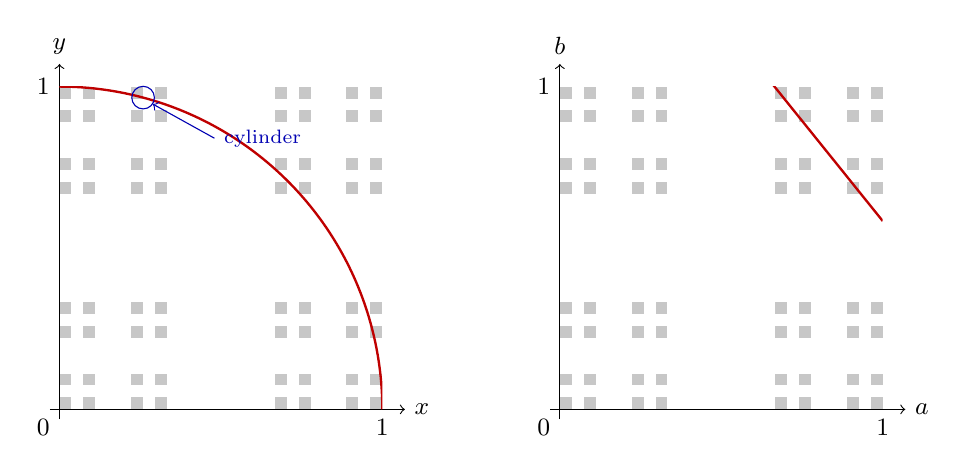
\begin{tikzpicture}[x=4.1cm,y=4.1cm,font=\small]
\begin{scope}[shift={(0.0,0)}]
\fill[black!22] (0.000000000,0.000000000) rectangle (0.037037037,0.037037037);
\fill[black!22] (0.000000000,0.074074074) rectangle (0.037037037,0.111111111);
\fill[black!22] (0.000000000,0.222222222) rectangle (0.037037037,0.259259259);
\fill[black!22] (0.000000000,0.296296296) rectangle (0.037037037,0.333333333);
\fill[black!22] (0.000000000,0.666666667) rectangle (0.037037037,0.703703704);
\fill[black!22] (0.000000000,0.740740741) rectangle (0.037037037,0.777777778);
\fill[black!22] (0.000000000,0.888888889) rectangle (0.037037037,0.925925926);
\fill[black!22] (0.000000000,0.962962963) rectangle (0.037037037,1.000000000);
\fill[black!22] (0.074074074,0.000000000) rectangle (0.111111111,0.037037037);
\fill[black!22] (0.074074074,0.074074074) rectangle (0.111111111,0.111111111);
\fill[black!22] (0.074074074,0.222222222) rectangle (0.111111111,0.259259259);
\fill[black!22] (0.074074074,0.296296296) rectangle (0.111111111,0.333333333);
\fill[black!22] (0.074074074,0.666666667) rectangle (0.111111111,0.703703704);
\fill[black!22] (0.074074074,0.740740741) rectangle (0.111111111,0.777777778);
\fill[black!22] (0.074074074,0.888888889) rectangle (0.111111111,0.925925926);
\fill[black!22] (0.074074074,0.962962963) rectangle (0.111111111,1.000000000);
\fill[black!22] (0.222222222,0.000000000) rectangle (0.259259259,0.037037037);
\fill[black!22] (0.222222222,0.074074074) rectangle (0.259259259,0.111111111);
\fill[black!22] (0.222222222,0.222222222) rectangle (0.259259259,0.259259259);
\fill[black!22] (0.222222222,0.296296296) rectangle (0.259259259,0.333333333);
\fill[black!22] (0.222222222,0.666666667) rectangle (0.259259259,0.703703704);
\fill[black!22] (0.222222222,0.740740741) rectangle (0.259259259,0.777777778);
\fill[black!22] (0.222222222,0.888888889) rectangle (0.259259259,0.925925926);
\fill[black!22] (0.222222222,0.962962963) rectangle (0.259259259,1.000000000);
\fill[black!22] (0.296296296,0.000000000) rectangle (0.333333333,0.037037037);
\fill[black!22] (0.296296296,0.074074074) rectangle (0.333333333,0.111111111);
\fill[black!22] (0.296296296,0.222222222) rectangle (0.333333333,0.259259259);
\fill[black!22] (0.296296296,0.296296296) rectangle (0.333333333,0.333333333);
\fill[black!22] (0.296296296,0.666666667) rectangle (0.333333333,0.703703704);
\fill[black!22] (0.296296296,0.740740741) rectangle (0.333333333,0.777777778);
\fill[black!22] (0.296296296,0.888888889) rectangle (0.333333333,0.925925926);
\fill[black!22] (0.296296296,0.962962963) rectangle (0.333333333,1.000000000);
\fill[black!22] (0.666666667,0.000000000) rectangle (0.703703704,0.037037037);
\fill[black!22] (0.666666667,0.074074074) rectangle (0.703703704,0.111111111);
\fill[black!22] (0.666666667,0.222222222) rectangle (0.703703704,0.259259259);
\fill[black!22] (0.666666667,0.296296296) rectangle (0.703703704,0.333333333);
\fill[black!22] (0.666666667,0.666666667) rectangle (0.703703704,0.703703704);
\fill[black!22] (0.666666667,0.740740741) rectangle (0.703703704,0.777777778);
\fill[black!22] (0.666666667,0.888888889) rectangle (0.703703704,0.925925926);
\fill[black!22] (0.666666667,0.962962963) rectangle (0.703703704,1.000000000);
\fill[black!22] (0.740740741,0.000000000) rectangle (0.777777778,0.037037037);
\fill[black!22] (0.740740741,0.074074074) rectangle (0.777777778,0.111111111);
\fill[black!22] (0.740740741,0.222222222) rectangle (0.777777778,0.259259259);
\fill[black!22] (0.740740741,0.296296296) rectangle (0.777777778,0.333333333);
\fill[black!22] (0.740740741,0.666666667) rectangle (0.777777778,0.703703704);
\fill[black!22] (0.740740741,0.740740741) rectangle (0.777777778,0.777777778);
\fill[black!22] (0.740740741,0.888888889) rectangle (0.777777778,0.925925926);
\fill[black!22] (0.740740741,0.962962963) rectangle (0.777777778,1.000000000);
\fill[black!22] (0.888888889,0.000000000) rectangle (0.925925926,0.037037037);
\fill[black!22] (0.888888889,0.074074074) rectangle (0.925925926,0.111111111);
\fill[black!22] (0.888888889,0.222222222) rectangle (0.925925926,0.259259259);
\fill[black!22] (0.888888889,0.296296296) rectangle (0.925925926,0.333333333);
\fill[black!22] (0.888888889,0.666666667) rectangle (0.925925926,0.703703704);
\fill[black!22] (0.888888889,0.740740741) rectangle (0.925925926,0.777777778);
\fill[black!22] (0.888888889,0.888888889) rectangle (0.925925926,0.925925926);
\fill[black!22] (0.888888889,0.962962963) rectangle (0.925925926,1.000000000);
\fill[black!22] (0.962962963,0.000000000) rectangle (1.000000000,0.037037037);
\fill[black!22] (0.962962963,0.074074074) rectangle (1.000000000,0.111111111);
\fill[black!22] (0.962962963,0.222222222) rectangle (1.000000000,0.259259259);
\fill[black!22] (0.962962963,0.296296296) rectangle (1.000000000,0.333333333);
\fill[black!22] (0.962962963,0.666666667) rectangle (1.000000000,0.703703704);
\fill[black!22] (0.962962963,0.740740741) rectangle (1.000000000,0.777777778);
\fill[black!22] (0.962962963,0.888888889) rectangle (1.000000000,0.925925926);
\fill[black!22] (0.962962963,0.962962963) rectangle (1.000000000,1.000000000);
\draw[->] (-.03,0)--(1.07,0);
\draw[->] (0,-.03)--(0,1.07);
\node[below left] at (0,0) {$0$};
\node[below] at (1,0) {$1$};
\node[left] at (0,1) {$1$};
\begin{scope}\clip (0,0) rectangle (1,1);
\draw[red!75!black,line width=.85pt] plot coordinates {
(1.0000000000,0.0000000000)
(0.9999691576,0.0078539009)
(0.9998766325,0.0157073173)
(0.9997224302,0.0235597648)
(0.9995065604,0.0314107591)
(0.9992290362,0.0392598158)
(0.9988898750,0.0471064507)
(0.9984890975,0.0549501799)
(0.9980267284,0.0627905195)
(0.9975027964,0.0706269859)
(0.9969173337,0.0784590957)
(0.9962703765,0.0862863658)
(0.9955619646,0.0941083133)
(0.9947921418,0.1019244558)
(0.9939609555,0.1097343111)
(0.9930684570,0.1175373975)
(0.9921147013,0.1253332336)
(0.9910997474,0.1331213385)
(0.9900236577,0.1409012319)
(0.9888864987,0.1486724339)
(0.9876883406,0.1564344650)
(0.9864292572,0.1641868466)
(0.9851093262,0.1719291003)
(0.9837286289,0.1796607486)
(0.9822872507,0.1873813146)
(0.9807852804,0.1950903220)
(0.9792228106,0.2027872954)
(0.9775999378,0.2104717598)
(0.9759167619,0.2181432414)
(0.9741733870,0.2258012669)
(0.9723699204,0.2334453639)
(0.9705064735,0.2410750608)
(0.9685831611,0.2486898872)
(0.9666001020,0.2562893731)
(0.9645574185,0.2638730500)
(0.9624552365,0.2714404499)
(0.9602936857,0.2789911060)
(0.9580728995,0.2865245527)
(0.9557930148,0.2940403252)
(0.9534541723,0.3015379599)
(0.9510565163,0.3090169944)
(0.9486001946,0.3164769672)
(0.9460853588,0.3239174182)
(0.9435121640,0.3313378885)
(0.9408807690,0.3387379202)
(0.9381913359,0.3461170571)
(0.9354440308,0.3534748438)
(0.9326390231,0.3608108265)
(0.9297764859,0.3681245527)
(0.9268565956,0.3754155712)
(0.9238795325,0.3826834324)
(0.9208454801,0.3899276878)
(0.9177546257,0.3971478906)
(0.9146071598,0.4043435955)
(0.9114032766,0.4115143586)
(0.9081431738,0.4186597375)
(0.9048270525,0.4257792916)
(0.9014551171,0.4328725815)
(0.8980275758,0.4399391699)
(0.8945446398,0.4469786207)
(0.8910065242,0.4539904997)
(0.8874134471,0.4609743745)
(0.8837656301,0.4679298143)
(0.8800632983,0.4748563899)
(0.8763066800,0.4817536741)
(0.8724960071,0.4886212415)
(0.8686315144,0.4954586684)
(0.8647134405,0.5022655331)
(0.8607420270,0.5090414158)
(0.8567175189,0.5157858983)
(0.8526401644,0.5224985647)
(0.8485102150,0.5291790010)
(0.8443279255,0.5358267950)
(0.8400935539,0.5424415367)
(0.8358073614,0.5490228180)
(0.8314696123,0.5555702330)
(0.8270805743,0.5620833779)
(0.8226405180,0.5685618507)
(0.8181497174,0.5750052520)
(0.8136084495,0.5814131843)
(0.8090169944,0.5877852523)
(0.8043756353,0.5941210629)
(0.7996846585,0.6004202253)
(0.7949443534,0.6066823510)
(0.7901550124,0.6129070537)
(0.7853169309,0.6190939493)
(0.7804304073,0.6252426563)
(0.7754957432,0.6313527954)
(0.7705132428,0.6374239897)
(0.7654832135,0.6434558647)
(0.7604059656,0.6494480483)
(0.7552818123,0.6554001709)
(0.7501110696,0.6613118653)
(0.7448940566,0.6671827669)
(0.7396310950,0.6730125135)
(0.7343225094,0.6788007455)
(0.7289686274,0.6845471059)
(0.7235697792,0.6902512402)
(0.7181262978,0.6959127966)
(0.7126385189,0.7015314258)
(0.7071067812,0.7071067812)
(0.7015314258,0.7126385189)
(0.6959127966,0.7181262978)
(0.6902512402,0.7235697792)
(0.6845471059,0.7289686274)
(0.6788007455,0.7343225094)
(0.6730125135,0.7396310950)
(0.6671827669,0.7448940566)
(0.6613118653,0.7501110696)
(0.6554001709,0.7552818123)
(0.6494480483,0.7604059656)
(0.6434558647,0.7654832135)
(0.6374239897,0.7705132428)
(0.6313527954,0.7754957432)
(0.6252426563,0.7804304073)
(0.6190939493,0.7853169309)
(0.6129070537,0.7901550124)
(0.6066823510,0.7949443534)
(0.6004202253,0.7996846585)
(0.5941210629,0.8043756353)
(0.5877852523,0.8090169944)
(0.5814131843,0.8136084495)
(0.5750052520,0.8181497174)
(0.5685618507,0.8226405180)
(0.5620833779,0.8270805743)
(0.5555702330,0.8314696123)
(0.5490228180,0.8358073614)
(0.5424415367,0.8400935539)
(0.5358267950,0.8443279255)
(0.5291790010,0.8485102150)
(0.5224985647,0.8526401644)
(0.5157858983,0.8567175189)
(0.5090414158,0.8607420270)
(0.5022655331,0.8647134405)
(0.4954586684,0.8686315144)
(0.4886212415,0.8724960071)
(0.4817536741,0.8763066800)
(0.4748563899,0.8800632983)
(0.4679298143,0.8837656301)
(0.4609743745,0.8874134471)
(0.4539904997,0.8910065242)
(0.4469786207,0.8945446398)
(0.4399391699,0.8980275758)
(0.4328725815,0.9014551171)
(0.4257792916,0.9048270525)
(0.4186597375,0.9081431738)
(0.4115143586,0.9114032766)
(0.4043435955,0.9146071598)
(0.3971478906,0.9177546257)
(0.3899276878,0.9208454801)
(0.3826834324,0.9238795325)
(0.3754155712,0.9268565956)
(0.3681245527,0.9297764859)
(0.3608108265,0.9326390231)
(0.3534748438,0.9354440308)
(0.3461170571,0.9381913359)
(0.3387379202,0.9408807690)
(0.3313378885,0.9435121640)
(0.3239174182,0.9460853588)
(0.3164769672,0.9486001946)
(0.3090169944,0.9510565163)
(0.3015379599,0.9534541723)
(0.2940403252,0.9557930148)
(0.2865245527,0.9580728995)
(0.2789911060,0.9602936857)
(0.2714404499,0.9624552365)
(0.2638730500,0.9645574185)
(0.2562893731,0.9666001020)
(0.2486898872,0.9685831611)
(0.2410750608,0.9705064735)
(0.2334453639,0.9723699204)
(0.2258012669,0.9741733870)
(0.2181432414,0.9759167619)
(0.2104717598,0.9775999378)
(0.2027872954,0.9792228106)
(0.1950903220,0.9807852804)
(0.1873813146,0.9822872507)
(0.1796607486,0.9837286289)
(0.1719291003,0.9851093262)
(0.1641868466,0.9864292572)
(0.1564344650,0.9876883406)
(0.1486724339,0.9888864987)
(0.1409012319,0.9900236577)
(0.1331213385,0.9910997474)
(0.1253332336,0.9921147013)
(0.1175373975,0.9930684570)
(0.1097343111,0.9939609555)
(0.1019244558,0.9947921418)
(0.0941083133,0.9955619646)
(0.0862863658,0.9962703765)
(0.0784590957,0.9969173337)
(0.0706269859,0.9975027964)
(0.0627905195,0.9980267284)
(0.0549501799,0.9984890975)
(0.0471064507,0.9988898750)
(0.0392598158,0.9992290362)
(0.0314107591,0.9995065604)
(0.0235597648,0.9997224302)
(0.0157073173,0.9998766325)
(0.0078539009,0.9999691576)
(0.0000000000,1.0000000000)
};
\end{scope}
\draw[blue!70!black] (0.25903064,0.96578266) circle[radius=.035];
\draw[blue!70!black,<-] (0.28903064,0.94578266)--(.48,.84);
\node[right,blue!70!black] at (.48,.84) {\scriptsize cylinder};
\node[right] at (1.07,0) {$x$};
\node[above] at (0,1.07) {$y$};
\end{scope}
\begin{scope}[shift={(1.55,0)}]
\fill[black!22] (0.000000000,0.000000000) rectangle (0.037037037,0.037037037);
\fill[black!22] (0.000000000,0.074074074) rectangle (0.037037037,0.111111111);
\fill[black!22] (0.000000000,0.222222222) rectangle (0.037037037,0.259259259);
\fill[black!22] (0.000000000,0.296296296) rectangle (0.037037037,0.333333333);
\fill[black!22] (0.000000000,0.666666667) rectangle (0.037037037,0.703703704);
\fill[black!22] (0.000000000,0.740740741) rectangle (0.037037037,0.777777778);
\fill[black!22] (0.000000000,0.888888889) rectangle (0.037037037,0.925925926);
\fill[black!22] (0.000000000,0.962962963) rectangle (0.037037037,1.000000000);
\fill[black!22] (0.074074074,0.000000000) rectangle (0.111111111,0.037037037);
\fill[black!22] (0.074074074,0.074074074) rectangle (0.111111111,0.111111111);
\fill[black!22] (0.074074074,0.222222222) rectangle (0.111111111,0.259259259);
\fill[black!22] (0.074074074,0.296296296) rectangle (0.111111111,0.333333333);
\fill[black!22] (0.074074074,0.666666667) rectangle (0.111111111,0.703703704);
\fill[black!22] (0.074074074,0.740740741) rectangle (0.111111111,0.777777778);
\fill[black!22] (0.074074074,0.888888889) rectangle (0.111111111,0.925925926);
\fill[black!22] (0.074074074,0.962962963) rectangle (0.111111111,1.000000000);
\fill[black!22] (0.222222222,0.000000000) rectangle (0.259259259,0.037037037);
\fill[black!22] (0.222222222,0.074074074) rectangle (0.259259259,0.111111111);
\fill[black!22] (0.222222222,0.222222222) rectangle (0.259259259,0.259259259);
\fill[black!22] (0.222222222,0.296296296) rectangle (0.259259259,0.333333333);
\fill[black!22] (0.222222222,0.666666667) rectangle (0.259259259,0.703703704);
\fill[black!22] (0.222222222,0.740740741) rectangle (0.259259259,0.777777778);
\fill[black!22] (0.222222222,0.888888889) rectangle (0.259259259,0.925925926);
\fill[black!22] (0.222222222,0.962962963) rectangle (0.259259259,1.000000000);
\fill[black!22] (0.296296296,0.000000000) rectangle (0.333333333,0.037037037);
\fill[black!22] (0.296296296,0.074074074) rectangle (0.333333333,0.111111111);
\fill[black!22] (0.296296296,0.222222222) rectangle (0.333333333,0.259259259);
\fill[black!22] (0.296296296,0.296296296) rectangle (0.333333333,0.333333333);
\fill[black!22] (0.296296296,0.666666667) rectangle (0.333333333,0.703703704);
\fill[black!22] (0.296296296,0.740740741) rectangle (0.333333333,0.777777778);
\fill[black!22] (0.296296296,0.888888889) rectangle (0.333333333,0.925925926);
\fill[black!22] (0.296296296,0.962962963) rectangle (0.333333333,1.000000000);
\fill[black!22] (0.666666667,0.000000000) rectangle (0.703703704,0.037037037);
\fill[black!22] (0.666666667,0.074074074) rectangle (0.703703704,0.111111111);
\fill[black!22] (0.666666667,0.222222222) rectangle (0.703703704,0.259259259);
\fill[black!22] (0.666666667,0.296296296) rectangle (0.703703704,0.333333333);
\fill[black!22] (0.666666667,0.666666667) rectangle (0.703703704,0.703703704);
\fill[black!22] (0.666666667,0.740740741) rectangle (0.703703704,0.777777778);
\fill[black!22] (0.666666667,0.888888889) rectangle (0.703703704,0.925925926);
\fill[black!22] (0.666666667,0.962962963) rectangle (0.703703704,1.000000000);
\fill[black!22] (0.740740741,0.000000000) rectangle (0.777777778,0.037037037);
\fill[black!22] (0.740740741,0.074074074) rectangle (0.777777778,0.111111111);
\fill[black!22] (0.740740741,0.222222222) rectangle (0.777777778,0.259259259);
\fill[black!22] (0.740740741,0.296296296) rectangle (0.777777778,0.333333333);
\fill[black!22] (0.740740741,0.666666667) rectangle (0.777777778,0.703703704);
\fill[black!22] (0.740740741,0.740740741) rectangle (0.777777778,0.777777778);
\fill[black!22] (0.740740741,0.888888889) rectangle (0.777777778,0.925925926);
\fill[black!22] (0.740740741,0.962962963) rectangle (0.777777778,1.000000000);
\fill[black!22] (0.888888889,0.000000000) rectangle (0.925925926,0.037037037);
\fill[black!22] (0.888888889,0.074074074) rectangle (0.925925926,0.111111111);
\fill[black!22] (0.888888889,0.222222222) rectangle (0.925925926,0.259259259);
\fill[black!22] (0.888888889,0.296296296) rectangle (0.925925926,0.333333333);
\fill[black!22] (0.888888889,0.666666667) rectangle (0.925925926,0.703703704);
\fill[black!22] (0.888888889,0.740740741) rectangle (0.925925926,0.777777778);
\fill[black!22] (0.888888889,0.888888889) rectangle (0.925925926,0.925925926);
\fill[black!22] (0.888888889,0.962962963) rectangle (0.925925926,1.000000000);
\fill[black!22] (0.962962963,0.000000000) rectangle (1.000000000,0.037037037);
\fill[black!22] (0.962962963,0.074074074) rectangle (1.000000000,0.111111111);
\fill[black!22] (0.962962963,0.222222222) rectangle (1.000000000,0.259259259);
\fill[black!22] (0.962962963,0.296296296) rectangle (1.000000000,0.333333333);
\fill[black!22] (0.962962963,0.666666667) rectangle (1.000000000,0.703703704);
\fill[black!22] (0.962962963,0.740740741) rectangle (1.000000000,0.777777778);
\fill[black!22] (0.962962963,0.888888889) rectangle (1.000000000,0.925925926);
\fill[black!22] (0.962962963,0.962962963) rectangle (1.000000000,1.000000000);
\draw[->] (-.03,0)--(1.07,0);
\draw[->] (0,-.03)--(0,1.07);
\node[below left] at (0,0) {$0$};
\node[below] at (1,0) {$1$};
\node[left] at (0,1) {$1$};
\begin{scope}\clip (0,0) rectangle (1,1);
\draw[red!75!black,line width=.85pt] plot coordinates {
(0.0000000000,1.8247969224)
(0.0025000000,1.8216973657)
(0.0050000000,1.8185977909)
(0.0075000000,1.8154981979)
(0.0100000000,1.8123985868)
(0.0125000000,1.8092989575)
(0.0150000000,1.8061993101)
(0.0175000000,1.8030996446)
(0.0200000000,1.7999999609)
(0.0225000000,1.7969002590)
(0.0250000000,1.7938005390)
(0.0275000000,1.7907008009)
(0.0300000000,1.7876010446)
(0.0325000000,1.7845012702)
(0.0350000000,1.7814014776)
(0.0375000000,1.7783016669)
(0.0400000000,1.7752018380)
(0.0425000000,1.7721019910)
(0.0450000000,1.7690021259)
(0.0475000000,1.7659022426)
(0.0500000000,1.7628023411)
(0.0525000000,1.7597024215)
(0.0550000000,1.7566024837)
(0.0575000000,1.7535025278)
(0.0600000000,1.7504025538)
(0.0625000000,1.7473025616)
(0.0650000000,1.7442025513)
(0.0675000000,1.7411025228)
(0.0700000000,1.7380024761)
(0.0725000000,1.7349024113)
(0.0750000000,1.7318023284)
(0.0775000000,1.7287022273)
(0.0800000000,1.7256021080)
(0.0825000000,1.7225019706)
(0.0850000000,1.7194018150)
(0.0875000000,1.7163016413)
(0.0900000000,1.7132014495)
(0.0925000000,1.7101012394)
(0.0950000000,1.7070010113)
(0.0975000000,1.7039007650)
(0.1000000000,1.7008005005)
(0.1025000000,1.6977002179)
(0.1050000000,1.6945999171)
(0.1075000000,1.6914995981)
(0.1100000000,1.6883992610)
(0.1125000000,1.6852989058)
(0.1150000000,1.6821985324)
(0.1175000000,1.6790981408)
(0.1200000000,1.6759977311)
(0.1225000000,1.6728973032)
(0.1250000000,1.6697968572)
(0.1275000000,1.6666963930)
(0.1300000000,1.6635959107)
(0.1325000000,1.6604954102)
(0.1350000000,1.6573948915)
(0.1375000000,1.6542943547)
(0.1400000000,1.6511937997)
(0.1425000000,1.6480932266)
(0.1450000000,1.6449926353)
(0.1475000000,1.6418920258)
(0.1500000000,1.6387913982)
(0.1525000000,1.6356907524)
(0.1550000000,1.6325900885)
(0.1575000000,1.6294894064)
(0.1600000000,1.6263887061)
(0.1625000000,1.6232879877)
(0.1650000000,1.6201872511)
(0.1675000000,1.6170864964)
(0.1700000000,1.6139857235)
(0.1725000000,1.6108849324)
(0.1750000000,1.6077841232)
(0.1775000000,1.6046832958)
(0.1800000000,1.6015824502)
(0.1825000000,1.5984815865)
(0.1850000000,1.5953807046)
(0.1875000000,1.5922798046)
(0.1900000000,1.5891788864)
(0.1925000000,1.5860779500)
(0.1950000000,1.5829769954)
(0.1975000000,1.5798760227)
(0.2000000000,1.5767750319)
(0.2025000000,1.5736740228)
(0.2050000000,1.5705729956)
(0.2075000000,1.5674719502)
(0.2100000000,1.5643708867)
(0.2125000000,1.5612698050)
(0.2150000000,1.5581687051)
(0.2175000000,1.5550675871)
(0.2200000000,1.5519664508)
(0.2225000000,1.5488652965)
(0.2250000000,1.5457641239)
(0.2275000000,1.5426629332)
(0.2300000000,1.5395617243)
(0.2325000000,1.5364604973)
(0.2350000000,1.5333592520)
(0.2375000000,1.5302579886)
(0.2400000000,1.5271567071)
(0.2425000000,1.5240554073)
(0.2450000000,1.5209540894)
(0.2475000000,1.5178527533)
(0.2500000000,1.5147513991)
(0.2525000000,1.5116500267)
(0.2550000000,1.5085486361)
(0.2575000000,1.5054472273)
(0.2600000000,1.5023458003)
(0.2625000000,1.4992443552)
(0.2650000000,1.4961428919)
(0.2675000000,1.4930414105)
(0.2700000000,1.4899399108)
(0.2725000000,1.4868383930)
(0.2750000000,1.4837368570)
(0.2775000000,1.4806353029)
(0.2800000000,1.4775337305)
(0.2825000000,1.4744321400)
(0.2850000000,1.4713305313)
(0.2875000000,1.4682289045)
(0.2900000000,1.4651272594)
(0.2925000000,1.4620255962)
(0.2950000000,1.4589239148)
(0.2975000000,1.4558222152)
(0.3000000000,1.4527204975)
(0.3025000000,1.4496187616)
(0.3050000000,1.4465170075)
(0.3075000000,1.4434152352)
(0.3100000000,1.4403134447)
(0.3125000000,1.4372116361)
(0.3150000000,1.4341098092)
(0.3175000000,1.4310079642)
(0.3200000000,1.4279061011)
(0.3225000000,1.4248042197)
(0.3250000000,1.4217023201)
(0.3275000000,1.4186004024)
(0.3300000000,1.4154984665)
(0.3325000000,1.4123965124)
(0.3350000000,1.4092945402)
(0.3375000000,1.4061925497)
(0.3400000000,1.4030905411)
(0.3425000000,1.3999885143)
(0.3450000000,1.3968864693)
(0.3475000000,1.3937844061)
(0.3500000000,1.3906823247)
(0.3525000000,1.3875802251)
(0.3550000000,1.3844781074)
(0.3575000000,1.3813759715)
(0.3600000000,1.3782738174)
(0.3625000000,1.3751716451)
(0.3650000000,1.3720694546)
(0.3675000000,1.3689672460)
(0.3700000000,1.3658650191)
(0.3725000000,1.3627627741)
(0.3750000000,1.3596605109)
(0.3775000000,1.3565582295)
(0.3800000000,1.3534559299)
(0.3825000000,1.3503536121)
(0.3850000000,1.3472512761)
(0.3875000000,1.3441489220)
(0.3900000000,1.3410465496)
(0.3925000000,1.3379441591)
(0.3950000000,1.3348417503)
(0.3975000000,1.3317393234)
(0.4000000000,1.3286368783)
(0.4025000000,1.3255344150)
(0.4050000000,1.3224319336)
(0.4075000000,1.3193294339)
(0.4100000000,1.3162269160)
(0.4125000000,1.3131243800)
(0.4150000000,1.3100218257)
(0.4175000000,1.3069192533)
(0.4200000000,1.3038166626)
(0.4225000000,1.3007140538)
(0.4250000000,1.2976114268)
(0.4275000000,1.2945087816)
(0.4300000000,1.2914061182)
(0.4325000000,1.2883034366)
(0.4350000000,1.2852007368)
(0.4375000000,1.2820980188)
(0.4400000000,1.2789952826)
(0.4425000000,1.2758925283)
(0.4450000000,1.2727897557)
(0.4475000000,1.2696869649)
(0.4500000000,1.2665841560)
(0.4525000000,1.2634813288)
(0.4550000000,1.2603784835)
(0.4575000000,1.2572756199)
(0.4600000000,1.2541727382)
(0.4625000000,1.2510698382)
(0.4650000000,1.2479669201)
(0.4675000000,1.2448639838)
(0.4700000000,1.2417610292)
(0.4725000000,1.2386580565)
(0.4750000000,1.2355550656)
(0.4775000000,1.2324520564)
(0.4800000000,1.2293490291)
(0.4825000000,1.2262459836)
(0.4850000000,1.2231429199)
(0.4875000000,1.2200398379)
(0.4900000000,1.2169367378)
(0.4925000000,1.2138336195)
(0.4950000000,1.2107304829)
(0.4975000000,1.2076273282)
(0.5000000000,1.2045241553)
(0.5025000000,1.2014209641)
(0.5050000000,1.1983177548)
(0.5075000000,1.1952145273)
(0.5100000000,1.1921112815)
(0.5125000000,1.1890080176)
(0.5150000000,1.1859047354)
(0.5175000000,1.1828014351)
(0.5200000000,1.1796981165)
(0.5225000000,1.1765947798)
(0.5250000000,1.1734914248)
(0.5275000000,1.1703880516)
(0.5300000000,1.1672846603)
(0.5325000000,1.1641812507)
(0.5350000000,1.1610778229)
(0.5375000000,1.1579743769)
(0.5400000000,1.1548709127)
(0.5425000000,1.1517674303)
(0.5450000000,1.1486639297)
(0.5475000000,1.1455604109)
(0.5500000000,1.1424568738)
(0.5525000000,1.1393533186)
(0.5550000000,1.1362497452)
(0.5575000000,1.1331461535)
(0.5600000000,1.1300425436)
(0.5625000000,1.1269389156)
(0.5650000000,1.1238352693)
(0.5675000000,1.1207316048)
(0.5700000000,1.1176279221)
(0.5725000000,1.1145242212)
(0.5750000000,1.1114205021)
(0.5775000000,1.1083167648)
(0.5800000000,1.1052130092)
(0.5825000000,1.1021092355)
(0.5850000000,1.0990054435)
(0.5875000000,1.0959016333)
(0.5900000000,1.0927978049)
(0.5925000000,1.0896939583)
(0.5950000000,1.0865900935)
(0.5975000000,1.0834862105)
(0.6000000000,1.0803823092)
(0.6025000000,1.0772783898)
(0.6050000000,1.0741744521)
(0.6075000000,1.0710704962)
(0.6100000000,1.0679665221)
(0.6125000000,1.0648625298)
(0.6150000000,1.0617585193)
(0.6175000000,1.0586544906)
(0.6200000000,1.0555504436)
(0.6225000000,1.0524463784)
(0.6250000000,1.0493422950)
(0.6275000000,1.0462381934)
(0.6300000000,1.0431340736)
(0.6325000000,1.0400299355)
(0.6350000000,1.0369257793)
(0.6375000000,1.0338216048)
(0.6400000000,1.0307174121)
(0.6425000000,1.0276132012)
(0.6450000000,1.0245089721)
(0.6475000000,1.0214047247)
(0.6500000000,1.0183004591)
(0.6525000000,1.0151961753)
(0.6550000000,1.0120918733)
(0.6575000000,1.0089875531)
(0.6600000000,1.0058832146)
(0.6625000000,1.0027788580)
(0.6650000000,0.9996744831)
(0.6675000000,0.9965700899)
(0.6700000000,0.9934656786)
(0.6725000000,0.9903612490)
(0.6750000000,0.9872568012)
(0.6775000000,0.9841523352)
(0.6800000000,0.9810478510)
(0.6825000000,0.9779433485)
(0.6850000000,0.9748388279)
(0.6875000000,0.9717342890)
(0.6900000000,0.9686297318)
(0.6925000000,0.9655251565)
(0.6950000000,0.9624205629)
(0.6975000000,0.9593159511)
(0.7000000000,0.9562113211)
(0.7025000000,0.9531066728)
(0.7050000000,0.9500020063)
(0.7075000000,0.9468973216)
(0.7100000000,0.9437926187)
(0.7125000000,0.9406878976)
(0.7150000000,0.9375831582)
(0.7175000000,0.9344784006)
(0.7200000000,0.9313736247)
(0.7225000000,0.9282688306)
(0.7250000000,0.9251640183)
(0.7275000000,0.9220591878)
(0.7300000000,0.9189543391)
(0.7325000000,0.9158494721)
(0.7350000000,0.9127445869)
(0.7375000000,0.9096396834)
(0.7400000000,0.9065347617)
(0.7425000000,0.9034298218)
(0.7450000000,0.9003248637)
(0.7475000000,0.8972198873)
(0.7500000000,0.8941148927)
(0.7525000000,0.8910098799)
(0.7550000000,0.8879048488)
(0.7575000000,0.8847997995)
(0.7600000000,0.8816947320)
(0.7625000000,0.8785896462)
(0.7650000000,0.8754845422)
(0.7675000000,0.8723794200)
(0.7700000000,0.8692742795)
(0.7725000000,0.8661691209)
(0.7750000000,0.8630639439)
(0.7775000000,0.8599587488)
(0.7800000000,0.8568535354)
(0.7825000000,0.8537483037)
(0.7850000000,0.8506430538)
(0.7875000000,0.8475377857)
(0.7900000000,0.8444324994)
(0.7925000000,0.8413271948)
(0.7950000000,0.8382218720)
(0.7975000000,0.8351165309)
(0.8000000000,0.8320111716)
(0.8025000000,0.8289057941)
(0.8050000000,0.8258003983)
(0.8075000000,0.8226949843)
(0.8100000000,0.8195895521)
(0.8125000000,0.8164841016)
(0.8150000000,0.8133786329)
(0.8175000000,0.8102731459)
(0.8200000000,0.8071676407)
(0.8225000000,0.8040621173)
(0.8250000000,0.8009565756)
(0.8275000000,0.7978510157)
(0.8300000000,0.7947454375)
(0.8325000000,0.7916398411)
(0.8350000000,0.7885342264)
(0.8375000000,0.7854285935)
(0.8400000000,0.7823229424)
(0.8425000000,0.7792172730)
(0.8450000000,0.7761115854)
(0.8475000000,0.7730058796)
(0.8500000000,0.7699001555)
(0.8525000000,0.7667944131)
(0.8550000000,0.7636886525)
(0.8575000000,0.7605828737)
(0.8600000000,0.7574770766)
(0.8625000000,0.7543712613)
(0.8650000000,0.7512654277)
(0.8675000000,0.7481595759)
(0.8700000000,0.7450537058)
(0.8725000000,0.7419478175)
(0.8750000000,0.7388419109)
(0.8775000000,0.7357359861)
(0.8800000000,0.7326300431)
(0.8825000000,0.7295240818)
(0.8850000000,0.7264181022)
(0.8875000000,0.7233121045)
(0.8900000000,0.7202060884)
(0.8925000000,0.7171000541)
(0.8950000000,0.7139940016)
(0.8975000000,0.7108879308)
(0.9000000000,0.7077818418)
(0.9025000000,0.7046757345)
(0.9050000000,0.7015696089)
(0.9075000000,0.6984634651)
(0.9100000000,0.6953573031)
(0.9125000000,0.6922511228)
(0.9150000000,0.6891449243)
(0.9175000000,0.6860387075)
(0.9200000000,0.6829324724)
(0.9225000000,0.6798262191)
(0.9250000000,0.6767199476)
(0.9275000000,0.6736136578)
(0.9300000000,0.6705073497)
(0.9325000000,0.6674010234)
(0.9350000000,0.6642946789)
(0.9375000000,0.6611883160)
(0.9400000000,0.6580819350)
(0.9425000000,0.6549755356)
(0.9450000000,0.6518691181)
(0.9475000000,0.6487626822)
(0.9500000000,0.6456562281)
(0.9525000000,0.6425497558)
(0.9550000000,0.6394432652)
(0.9575000000,0.6363367563)
(0.9600000000,0.6332302292)
(0.9625000000,0.6301236838)
(0.9650000000,0.6270171202)
(0.9675000000,0.6239105383)
(0.9700000000,0.6208039382)
(0.9725000000,0.6176973198)
(0.9750000000,0.6145906831)
(0.9775000000,0.6114840282)
(0.9800000000,0.6083773550)
(0.9825000000,0.6052706636)
(0.9850000000,0.6021639539)
(0.9875000000,0.5990572259)
(0.9900000000,0.5959504797)
(0.9925000000,0.5928437152)
(0.9950000000,0.5897369325)
(0.9975000000,0.5866301315)
(1.0000000000,0.5835233122)
};
\end{scope}
\node[right] at (1.07,0) {$a$};
\node[above] at (0,1.07) {$b$};
\end{scope}
\end{tikzpicture}

\caption{The Cantor dust \(C\times C\) and the unit circle \(S^1\)
(left), with a local cylinder shown on the right.}
\label{fig:source}
\end{figure}

A direct antecedent is Yu's study of missing-digit points near
manifolds~\cite{Yu2023}. He asked whether the unit circle contains
infinitely many points whose coordinates lie in the Cantor set of
contraction ratio \(1/5\), and also raised the problem of solving
\(x^3+y^3=1\) in the middle-third Cantor set. These questions concern
prescribed nonlinear curves. The intersection methods developed by
Shmerkin~\cite{Shmerkin2019} and Wu~\cite{Wu2019} provide relevant
dimension estimates, but, as Yu observed, even a zero-dimensional
upper bound does not establish finiteness. For the middle-third Cantor
set, Du, Jiang and Yao~\cite{DuJiangYao2025} subsequently proved, with
computer assistance, that \(x^2+y^2=1\) has at least \(10,000,000\)
distinct solutions with an irrational coordinate. This gave a large
finite lower bound without settling infinitude.

Jiang, Kong, Li and Wang~\cite{Jiang2026} then studied the unit-circle
intersection across the family of \(\lambda\)-Cantor sets. They proved
that only the two axis points occur for \(0<\lambda\leq2-\sqrt3\),
answering Yu's \(1/5\) question negatively, and gave sufficient ranges
for nontrivial intersections and continuum cardinality. They left
infinitude at \(\lambda=1/3\) open and asked for the Hausdorff dimension,
conjecturing \(2\log2/\log3-1\)~\cite[Question~5.1]{Jiang2026}.
More recently, Li, Shen and Wu~\cite{LiShenWu2026} established continuum
cardinality for \((\sqrt3-1)/2<\lambda<1/2\) and positive Hausdorff
dimension for \(\sqrt2-1<\lambda<1/2\). Their paper also includes an
infinitude theorem covering \(\lambda=1/3\), although their
positive-dimension range does not include this parameter. Our
unit-circle result strengthens the known infinitude at \(1/3\) to
positive Hausdorff dimension; the exact dimension remains open.
See also~\cite{HuntKanYorke1993,FengHuangRao2014,HuangKong2023}
for related results on Cantor-set intersections,
\cite{JiangNonlinear,McDonaldTaylor,MoreiraImages} on nonlinear images
of products of Cantor sets, and
\cite{PeresShmerkin2009,NazarovPeresShmerkin} on resonance and the
dimensions of arithmetic sums and convolutions.

Motivated by this question, we seek both to answer it and to understand
the phenomenon in a broader setting.
We replace the exponent \(2\) by a real parameter \(\alpha>1\) and the
middle-third Cantor set by a \(\lambda\)-Cantor set, and study the
solutions of \(x^\alpha+y^\alpha=1\) as these two parameters vary.








%%%%%%%%%%%%%%%%%%%%%%%%%%%%%%%%%%%%%%%%%%%%%%%%%%%%%%%
\subsection{Main Results}\label{subsec:main-results}


The question posed in~\cite{Jiang2026} asks about both the cardinality
and the dimension of the unit-circle intersection in the middle-third
Cantor dust. To understand how the solution set depends on the exponent
and the Cantor set, we ask two questions:
\begin{itemize}
\item (Q1) What happens if we replace the exponent \(2\) by \(\alpha\), even
allowing \(\alpha\) to be real? This will tell us whether the structure of
the solution set depends on the arithmetic structure of the integers.
\item (Q2) If we consider the more general \(\lambda\)-Cantor sets, when
is the solution set zero-dimensional, and when does it have positive
dimension? What do the transitions between these regimes look like
(the Hausdorff phase transitions discussed below)?
\end{itemize}



To answer (Q1), for \(0<\lambda\leq1/2\), we write
\[
C_\lambda:=
\left\{(1-\lambda)\sum_{j=1}^{\infty}
       \varepsilon_j\lambda^{j-1}:\varepsilon_j\in\{0,1\}\right\}.
\]
For \(\alpha>1\), define
\[
E_{\alpha,\lambda}:=
\{(x,y)\in C_\lambda\times C_\lambda:x^\alpha+y^\alpha=1\}.
\]

For \(\lambda=1/3\), we prove in Section~\ref{subsec:classical}
that the solution set has positive Hausdorff dimension for every
real exponent \(\alpha>1\).

\begin{theorem}\label{intro:integer-powers}
For every real \(\alpha>1\), \(\dim_{\mathrm H}(E_{\alpha,1/3})>0\).
\end{theorem}

Taking \(\alpha=2\) strengthens the known infinitude of the unit-circle
intersection to positive Hausdorff dimension. Section~\ref{sec:special}
gives a purely analytic proof of positive dimension in this case.
For general exponents, we give an analytic proof for irrational
\(\alpha\) and a computer-assisted proof for rational \(\alpha\).
The latter combines analytic criteria with exact finite covers and
strict-return certificates, documented in the
\href{https://github.com/Nero-17/LEAN-Formalisation-solutions-of-fermat-cantor-equation/blob/9ec893bcef7a71504234be897a16949c0a1f8313/docs/certificate-guide.pdf}{certificate reader's guide}.

Section~\ref{subsec:irrational} proves that, for every real exponent
\(\alpha>1\), the dimension is zero when \(0<\lambda\leq1/4\).
For every irrational exponent, each nonempty open interval in
\((1/4,1/2)\) contains a set of positive Lebesgue measure of
parameters for which the dimension is positive. Thus, for irrational
exponents, positive dimension occurs arbitrarily close to \(1/4\)
from above.
For \(\alpha>1\), we describe the first and last transition parameters by
\[
\begin{aligned}
\lambda_{\min}(\alpha)&:=
\inf\{\lambda\in(0,1/2]:\dim_{\mathrm H}(E_{\alpha,\lambda})>0\},\\
\lambda_{\max}(\alpha)&:=
\sup\{\lambda\in(0,1/2]:\dim_{\mathrm H}(E_{\alpha,\lambda})=0\}.
\end{aligned}
\]


We refer to this change from zero to positive Hausdorff dimension as
a \emph{Hausdorff phase transition}.
We call \(\lambda_{\min}\) and \(\lambda_{\max}\) the first and last
Hausdorff phase transition parameters, respectively.
In familiar models of statistical physics, we usually have a single
phase transition point: one phase throughout the parameter range
below it and a different phase throughout the range above it.
In more complicated models, however, there may be several phase
transition points, or even infinitely many. It is therefore natural
to ask whether, for \(\alpha=2\), there are multiple phase transition
points as \(\lambda\) varies.

The first transition satisfies the following bound.
\begin{theorem}\label{intro:irrational-onset}
For every real \(\alpha>1\), \(\lambda_{\min}(\alpha)\geq1/4\),
with equality whenever \(\alpha\) is irrational.
\end{theorem}



This theorem gives an initial picture of the solution sets across
the parameter family. It suggests considering a Hausdorff phase
transition diagram, with \(\alpha\) on the horizontal axis and \(\lambda\)
on the vertical axis. The diagram records how the two parameters
together determine the changes between zero and positive dimension.

Section~\ref{sec:last} develops this diagram and addresses (Q2).
We obtain an upper bound for the last Hausdorff phase transition
that holds for every real exponent \(\alpha>1\).
Above this common bound, the intersection has positive Hausdorff
dimension throughout the remaining contraction interval.

\begin{theorem}\label{intro:last-real}
For every real \(\alpha>1\),
\[
\lambda_{\max}(\alpha)<\frac{\sqrt3-1}{2}.
\]
\end{theorem}

Beyond positivity, we would like to determine the dimension itself.
The expected value in the positive-dimensional regime is
$
\frac{2\log2}{\log(1/\lambda)}-1,
$
the dimension of the Cantor dust minus one. At \(\lambda=1/3\),
this reduces to \(2\log2/\log3-1\), the value conjectured for the
unit-circle intersection by Jiang, Kong, Li and Wang
in~\cite[Question~5.1]{Jiang2026}.
Determining the dimension at every point of the diagram remains
difficult. Nevertheless, we obtain this formula for almost every
contraction ratio in an explicit interval, for each fixed irrational
exponent.

\begin{theorem}\label{intro:ae-dimension}
For every fixed irrational \(\alpha>1\), for Lebesgue almost every
\(\lambda\in(\sqrt3/4,1/2)\),
\[
\dim_{\mathrm H}(E_{\alpha,\lambda})
=\frac{2\log2}{\log(1/\lambda)}-1.
\]
\end{theorem}

This establishes the expected formula in the stated parameter range;
the precise dimension of the original unit-circle intersection in
the middle-third Cantor dust remains open.



These results provide a framework for studying intersections of the
curves \(x^\alpha+y^\alpha=1\) with \(\lambda\)-Cantor dust and their Hausdorff
phase transitions. Figure~\ref{fig:phase-diagram} summarises the
proved results and numerical estimates in a phase diagram.


\begin{figure}[H]
\centering
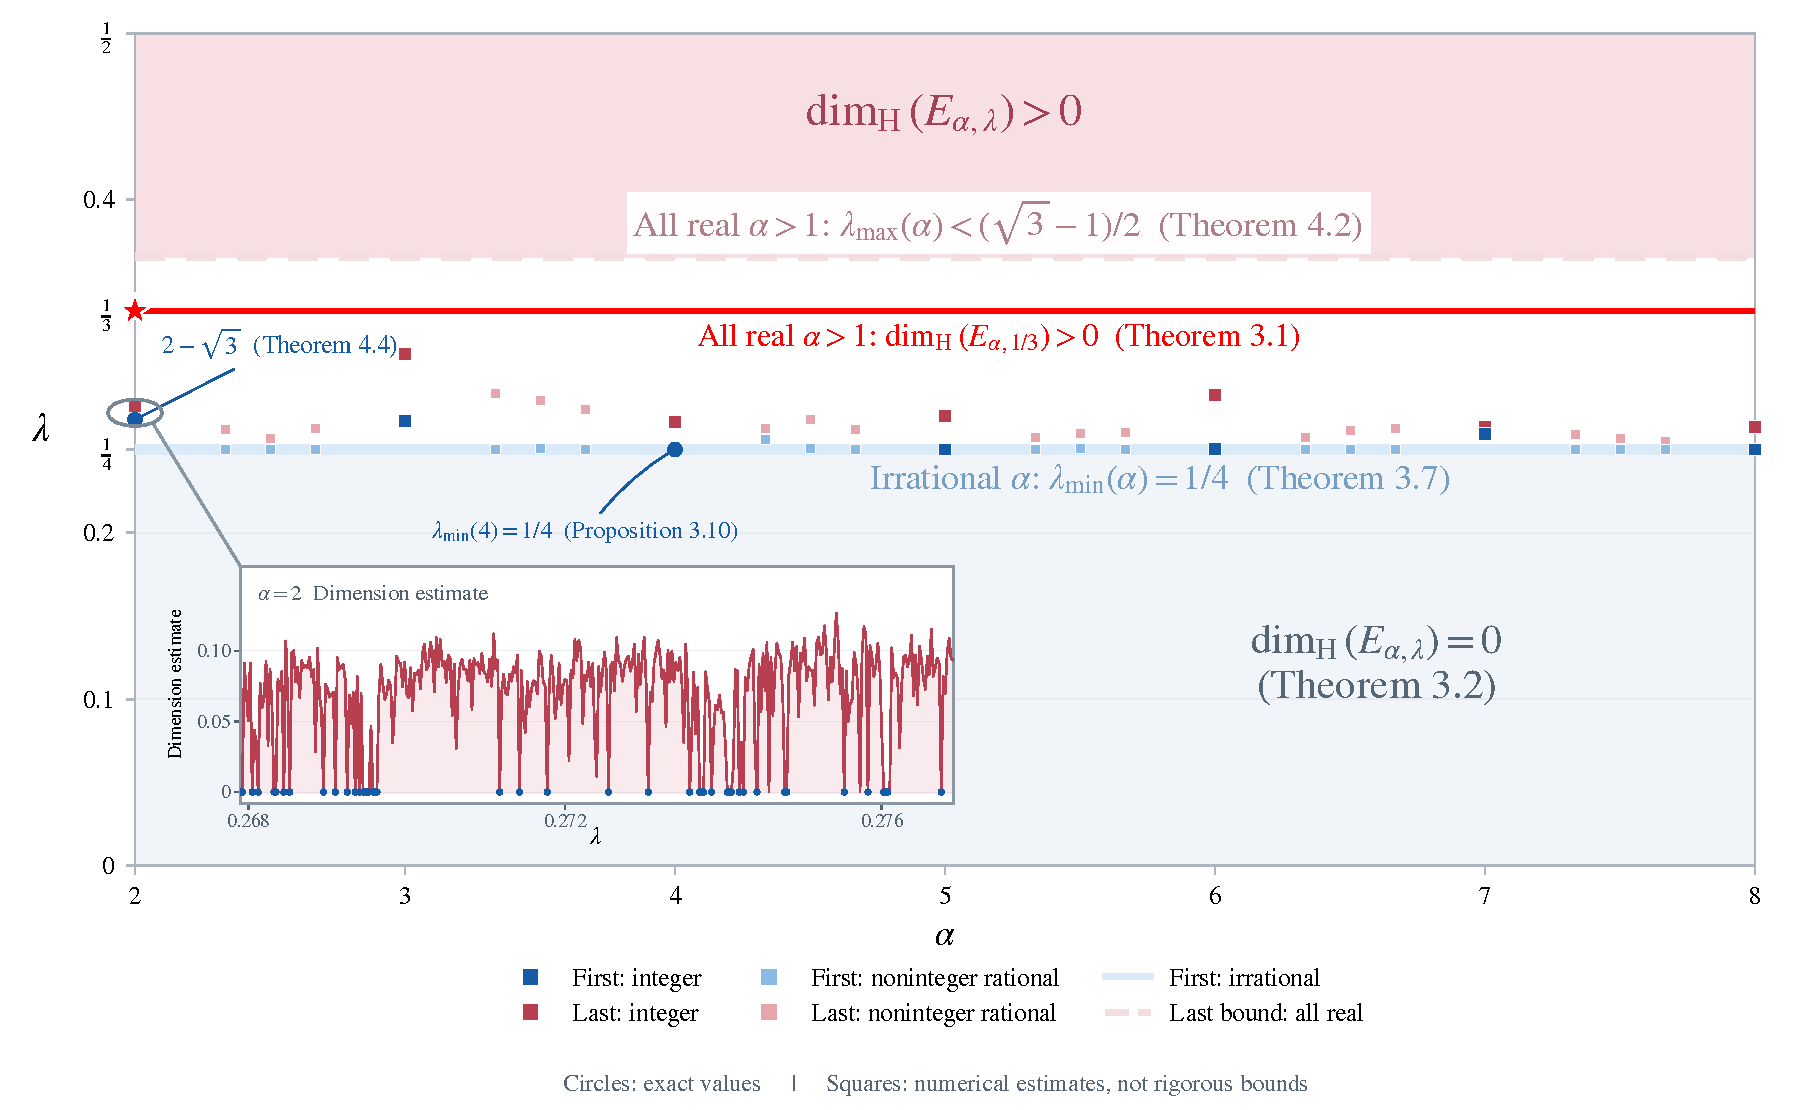
\includegraphics[width=\textwidth]{figures/phase-diagram.pdf}
\caption{Hausdorff phase transition diagram}
\label{fig:phase-diagram}
\end{figure}






\section{\texorpdfstring{\(x^2+y^2=1\)}{x2 + y2 = 1} in the middle-third Cantor set}\label{sec:special}


Our goal in this section is to prove that \(\dim_{\mathrm H}(E_{2,1/3})>0\).

We first locate a nonempty intersection in a pair of Cantor cylinders
and use returns between smaller cylinders to construct a perfect subset.
Strict returns persist under the nonlinear perturbation of the circle
and yield a branching construction of positive Hausdorff dimension,
proving the positivity assertion in
Theorem~\ref{thm:circle-quantitative}.


\begin{definition}\label{def:cantor-circle}
For the following unit-circle construction, write
\[
C:=C_{1/3}
=\left\{\sum_{j=1}^{\infty}\frac{2\varepsilon_j}{3^j}:
                \varepsilon_j\in\{0,1\}\right\},
\qquad
E:=E_{2,1/3}.
\]
\end{definition}

The proof uses a specific Cantor cylinder. Consider points of the form
\[
x=\frac{566+b}{3^7},\qquad y=\frac{6336+a}{3^8},
\qquad a,b\in C.
\]
The integers \(566\) and \(6336\), written as ternary words of lengths
seven and eight, are \(0202222\) and \(22200200\).
The circle equation in these coordinates is
\[
(6336+a)^2+9(566+b)^2=3^{16}.
\]
At \((a,b)=(0,0)\) and \((1,1)\), the left side minus \(3^{16}\)
equals \(-18621\) and \(4249\), respectively.
These signs alone only show a crossing of the ordinary square.
Lemma~\ref{lem:interval-cover} proves that every retained Cantor square maps
onto its entire corner-value interval, which makes the crossing a
point of the Cantor product.


The second ingredient concerns isolated points. Throughout the selected
cylinder, the normal ratio \(y/(3x)\) lies strictly between \(11/9\)
and \(2027/1624\). In this interval, a four-digit expansion that is
asymptotically confined to the regions with only one possible first
digit must eventually be periodic. We prove this assertion directly
in Lemma~\ref{lem:periodicity}. An exact quadratic expansion then transfers
it to any hypothetical isolated circle point.
Such a point would have rational coordinates, whereas
Lemma~\ref{lem:rational} proves that the only rational points of \(E\)
are the two axis points. Thus the selected compact intersection has
no isolated points.

This argument establishes cardinality. It does not give a positive
Hausdorff dimension bound, nor does it exclude quadratic irrational
numbers from \(C\). Both distinctions matter: a perfect compact set
can have zero Hausdorff dimension, and periodicity here follows from
isolation in a particular two-coordinate level set.

\paragraph{Rational points on the unit circle.}\label{sec:rational}

We first record the arithmetic obstruction that will rule out isolated
points at the end of the proof.

\begin{lemma}\label{lem:rational}
The rational points of \(E\) are exactly \((0,1)\) and \((1,0)\).
\end{lemma}

\begin{proof}
Suppose that \(x,y\) are rational, belong to \(C\), and satisfy
\(x^2+y^2=1\). If either coordinate is zero, the conclusion follows.
We may therefore assume that \(0<x,y<1\).
Choose a common denominator and write
\[
x=\frac{p}{d},\qquad y=\frac{q}{d},\qquad
p^2+q^2=d^2,\qquad \gcd(p,q,d)=1.
\]
If \(3\mid d\), reduction modulo \(3\) forces \(3\mid p,q\), a
contradiction. Hence \(d\) is coprime to \(3\).

Both ternary expansions are consequently purely periodic.
Indeed, choose \(k\geq1\) such that \(3^k\equiv1\pmod d\).
Multiplication by \(3^k\) preserves the fractional part of each
coordinate. Neither coordinate is a noninteger triadic rational, so
there is no endpoint ambiguity in its expansion.
Since the digits belong to \(\{0,2\}\), dividing the two period
numerators by \(2\) gives
\[
x=\frac{A}{N},\qquad y=\frac{B}{N},
\qquad N:=\frac{3^k-1}{2},
\]
where the ternary digits of \(A,B\) belong to \(\{0,1\}\).
All \(k\) ternary digits of \(N\) are \(1\), and
\[
A^2+B^2=N^2.
\]
Modulo \(3\), exactly one of \(A,B\) is \(1\).
After interchanging the coordinates, assume that
\(A\equiv1\pmod3\) and \(B\equiv0\pmod3\).

Let \(j\geq1\) be the exact exponent of \(3\) dividing \(B\).
The identity
\[
(N-A)(N+A)=B^2
\]
and \(N+A\equiv2\pmod3\) show that the exact exponent of \(3\)
dividing \(N-A\) is \(2j\).
Subtracting \(A\) from the all-one ternary expansion of \(N\)
requires no borrowing. Thus \(N-A\) has only \(0\) and \(1\) as
ternary digits, and its first nonzero digit is \(1\).
It follows that
\[
\frac{N-A}{3^{2j}}\equiv1\pmod3.
\]
Dividing the product identity by \(3^{2j}\) now gives a contradiction
modulo \(3\): its left side is \(1\cdot2\), while its right side is
a nonzero square. This excludes \(0<x,y<1\).
\end{proof}

\paragraph{A nonempty local intersection.}\label{sec:source}

We need a crossing criterion for actual Cantor points, valid in every
descendant square. The following elementary covering argument provides
it.

Let \(G\) be continuously differentiable on \([0,1]^2\). For ternary
words of the same length \(n\), with digits in \(\{0,2\}\), let \(u,v\)
be the corresponding left endpoints. The associated square and Cantor
product are
\[
Q:=[u,u+3^{-n}]\times[v,v+3^{-n}],
\qquad
(u+3^{-n}C)\times(v+3^{-n}C).
\]

\begin{lemma}\label{lem:interval-cover}
Suppose that
\[
0<\min_{[0,1]^2}G_b
\leq\max_{[0,1]^2}G_b
<\min_{[0,1]^2}G_a,
\qquad
\max_{[0,1]^2}G_a<3\min_{[0,1]^2}G_b.
\]
Then every square \(Q\) described above satisfies
\[
G\bigl((u+3^{-n}C)\times(v+3^{-n}C)\bigr)
=[G(u,v),G(u+3^{-n},v+3^{-n})].
\]
\end{lemma}

\begin{proof}
Write \(h\) for the side length of a retained square with lower-left
corner \((u,v)\). Its four children have lower-left offsets
\[
(0,0),\quad(0,2h/3),\quad(2h/3,0),\quad(2h/3,2h/3).
\]
Positivity of both partial derivatives implies that the image of each
ordinary child square is the interval between its lower-left and
upper-right corner values. Both sets of endpoints occur in the
displayed order, since increasing the first coordinate by \(2h/3\)
and decreasing the second by \(2h/3\) increases \(G\).

The first two intervals overlap because
\[
G(u+h/3,v+h/3)-G(u,v+2h/3)
\geq\frac h3\bigl(\min G_a-\max G_b\bigr)>0.
\]
The middle two overlap because
\[
G(u+h/3,v+h)-G(u+2h/3,v)
\geq h\min G_b-\frac h3\max G_a>0.
\]
The last two overlap by the same estimate as the first two.
Their union is therefore the whole parent corner-value interval.

Given any value in this interval, choose a child whose corner-value
interval contains it and repeat. The resulting nested closed squares
have diameters tending to zero. Their common point belongs to the
retained Cantor product, and continuity gives the prescribed value.
The same argument applies inside every descendant square.
\end{proof}

For the remainder of this construction, define
\[
F(a,b):=(6336+a)^2+9(566+b)^2
\]
and
\[
S:=\left\{\left(\frac{566+b}{3^7},\frac{6336+a}{3^8}\right):
                       a,b\in C,\ F(a,b)=3^{16}\right\}.
\]
The two allowed ternary prefixes show that \(S\subset E\).

\begin{proposition}\label{prop:source}
The set \(S\) is nonempty and compact.
\end{proposition}

\begin{proof}
On \([0,1]^2\),
\[
12672\leq F_a\leq12674,\qquad
10188\leq F_b\leq10206.
\]
In particular, \(12672>10206\) and \(12674<3\cdot10188\), so
Lemma~\ref{lem:interval-cover} applies. Since
\[
F(0,0)-3^{16}=-18621,\qquad
F(1,1)-3^{16}=4249,
\]
there is a point of \(C\times C\) with value \(3^{16}\).
Compactness follows from continuity and compactness of \(C\times C\).
\end{proof}

We will use two consequences of this calculation.
First, a retained square contains a point of
\(F(a,b)=3^{16}\) in its Cantor product if and only if its corner
values bracket \(3^{16}\), with equality allowed.
Second, throughout the entire source rectangle,
\begin{equation}\label{eq:normal-band}
\frac{11}{9}<\frac{704}{567}
\leq\frac{6336+a}{9(566+b)}
=\frac{y}{3x}
\leq\frac{6337}{5094}<\frac{2027}{1624}.
\end{equation}
The strict endpoint margins are \(11/567\) and
\(17125/4136328\), respectively.

\paragraph{Eventual periodicity of digit sequences.}\label{sec:digits}

Fix a real number
\begin{equation}\label{eq:r-band}
\frac{11}{9}<r<\frac{2027}{1624}.
\end{equation}
For a sequence \(c_n\in\{0,1,r,r+1\}\), indexed by \(n\geq0\), define
\[
T_n:=\sum_{j=0}^{\infty}\frac{c_{n+j}}{3^{j+1}}.
\]
Thus \(T_{n+1}=3T_n-c_n\).
The intervals relevant to a single admissible first digit are
\begin{equation}\label{eq:exclusive-domains}
\begin{aligned}
I_0&:=[0,1/3],
&I_1&:=[(r+1)/6,r/3],\\
I_r&:=[(r+3)/6,(r+1)/3],
&I_{r+1}&:=[(3r+1)/6,(r+1)/2].
\end{aligned}
\end{equation}
They are closed: the argument below must allow errors from curvature
and cannot discard their endpoints.

\begin{lemma}\label{lem:periodicity}
For \(r\) satisfying \eqref{eq:r-band}, the sequence \((c_n)\) is
eventually periodic whenever
\[
\lim_{n\to\infty}\operatorname{dist}(T_n,I_{c_n})=0.
\]
\end{lemma}

\begin{proof}
Put \(\delta_n:=\operatorname{dist}(T_n,I_{c_n})\).
Every exclusion below has a strictly positive margin depending only
on the fixed parameter \(r\). Because
\(\displaystyle\lim_{n\to\infty}\delta_n=0\), these exclusions hold
simultaneously after a sufficiently large index.
The reflection
\[
T_n\longmapsto\frac{r+1}{2}-T_n,\qquad
c_n\longmapsto r+1-c_n
\]
preserves the hypotheses and exchanges the digits \(0,r+1\) and \(1,r\).

If \(c_n=1\), then \(T_{n+1}\leq r-1+3\delta_n\).
Every domain for a nonzero next digit has lower endpoint at least
\((r+1)/6\). Hence \(c_{n+1}\ne0\) would imply
\[
\frac{7-5r}{6}\leq3\delta_n+\delta_{n+1}.
\]
The left side is positive, so sufficiently late occurrences of \(1\)
must be followed by \(0\). Reflection shows that sufficiently late
occurrences of \(r\) must be followed by \(r+1\).

After the pair \(10\), the recurrence gives
\[
\frac{3(r-1)}2-9\delta_n
\leq T_{n+2}=9T_n-3
\leq3(r-1)+9\delta_n.
\]
This excludes the next digit \(0\) or \(r+1\) at sufficiently late
indices, since the respective separating margins are
\[
\frac{3(r-1)}2-\frac13=\frac{9r-11}{6}>0,
\qquad
\frac{3r+1}{6}-3(r-1)=\frac{19-15r}{6}>0.
\]
The latter inequality uses \(2027/1624<19/15\).
The reflected conclusion holds after the pair \(r(r+1)\).
Consequently, once a middle digit \(1\) or \(r\) occurs sufficiently
late, the entire subsequent sequence consists of the two blocks
\[
10,\qquad r(r+1).
\]

Call these the low block and the high block.
An infinite sequence of low blocks has value \(3/8\).
If three successive blocks are low, high, high, then replacing all
other blocks by low blocks gives the lower bound
\[
T_n\geq\frac38+(4r-2)\left(\frac1{81}+\frac1{729}\right)
       =\frac38+\frac{20(2r-1)}{729}.
\]
Its first digit is \(1\), which also requires \(T_n\leq r/3+\delta_n\).
But
\[
\frac38+\frac{20(2r-1)}{729}-\frac r3
=\frac{2027-1624r}{5832}>0.
\]
Thus low, high, high is eventually forbidden, and reflection also
forbids high, low, low.
A binary sequence avoiding these two words is eventually constant
or alternating: after its first change, either forbidden word would
appear if the next symbol did not change again.
The original digit sequence is therefore eventually periodic.

It remains to consider a tail containing only \(0\) and \(r+1\).
At an occurrence of \(0,(r+1),(r+1)\), the terminal digit's domain
and the recurrence give
\[
T_n=\frac{r+1+T_{n+2}}9
\geq\frac{9r+7}{54}-\frac{\delta_{n+2}}9.
\]
The initial digit \(0\) requires \(T_n\leq1/3+\delta_n\).
These inequalities contradict one another for sufficiently large \(n\),
because
\[
\frac{9r+7}{54}-\frac13=\frac{9r-11}{54}>0.
\]
Reflection excludes \((r+1),0,0\) as well.
The same binary-word argument proves eventual constancy or alternation
in this case.
\end{proof}

The hypothesis of Lemma~\ref{lem:periodicity} permits arbitrary
vanishing errors. In particular, it applies when the domains arise
as linear approximations to a curved level set. This is the reason
for retaining the error terms throughout the proof.

\paragraph{The perfect subset and uncountability.}\label{sec:main}

We now combine the local covering property with the digit lemma.

\begin{theorem}\label{thm:main}
The set \(E\) has cardinality \(2^{\aleph_0}\).
\end{theorem}

\begin{proof}
By Proposition~\ref{prop:source}, \(S\) is a nonempty compact subset
of \(E\). We will show that \(S\) has no isolated points.
Suppose to the contrary that
\[
(x,y)=\left(\frac{566+b}{3^7},\frac{6336+a}{3^8}\right)\in S
\]
is isolated. Fix its normal ratio
\[
r:=\frac{6336+a}{9(566+b)}=\frac{y}{3x}.
\]
By \eqref{eq:normal-band}, this fixed value satisfies
\eqref{eq:r-band}.

Let \(a_n,b_n\in C\) be the tails of the allowed ternary expansions
of \(a,b\) after their first \(n\) digits. Write their next digits as
\(2\xi_n,2\beta_n\), where \(\xi_n,\beta_n\in\{0,1\}\).
Then
\[
a_n=\frac{2\xi_n+a_{n+1}}3,\qquad
b_n=\frac{2\beta_n+b_{n+1}}3.
\]
Define
\[
T_n:=\frac{ra_n+b_n}{2},\qquad c_n:=r\xi_n+\beta_n.
\]
These are precisely the tails and digits introduced before Lemma~\ref{lem:periodicity};
in particular, \(T_{n+1}=3T_n-c_n\) holds exactly.

The retained square of depth \(n\) containing \((a,b)\) can be
parametrised by
\[
\bigl(a+3^{-n}(s-a_n),\,b+3^{-n}(t-b_n)\bigr),
\qquad s,t\in[0,1].
\]
The quadratic expansion is exact:
\begin{align}
&\frac{F\bigl(a+3^{-n}(s-a_n),\,b+3^{-n}(t-b_n)\bigr)-F(a,b)}
       {36(566+b)3^{-n}}\notag\\
&\hspace{12mm}=\frac{rs+t}{2}-T_n
 +\frac{3^{-n}\bigl((s-a_n)^2+9(t-b_n)^2\bigr)}{36(566+b)}.
\label{eq:taylor}
\end{align}
The final term lies between zero and
\[
\eta_n:=\frac{5}{10188}\,3^{-n}.
\]
The normal \(r\) is held fixed at the original point throughout this
calculation; it is not replaced by a normal at a cylinder corner.

For a child with digit label \(c\in\{0,1,r,r+1\}\), the linear function
\((rs+t)/2\) takes values in
\[
J_c:=\left[\frac c3,\frac c3+\frac{r+1}{6}\right].
\]
If \(T_n\) is more than \(\eta_n\) from both endpoints inside \(J_c\),
the left side of \eqref{eq:taylor} has opposite signs at the child's
lower-left and upper-right corners. Lemma~\ref{lem:interval-cover}
then supplies an actual point of the Cantor product on the level
\(F=3^{16}\) in this child.

Because the original point is isolated, every sufficiently deep
retained square containing it has exactly one child containing a
point of that level set. The retained intervals at any fixed depth
are disjoint, including their endpoints, so a point in a different
child would be a different point of \(S\).
The original point belongs to its prescribed child, and therefore
\(T_n\in J_{c_n}\) exactly.

We claim that for all sufficiently large \(n\),
\begin{equation}\label{eq:approx-exclusive}
\operatorname{dist}(T_n,I_{c_n})\leq\eta_n.
\end{equation}
Here the \(I_c\) are the closed intervals in
\eqref{eq:exclusive-domains}.
Choose \(n\) so large that
\(\eta_n<\min\{1/3,(r-1)/3\}\).
If \(c_n=0\) and \(T_n>1/3+\eta_n\), then \(T_n\) is more than
\(\eta_n\) inside \(J_1\); its distance from the other endpoint of
\(J_1\) is at least \(1/3\).
This would give a point in a competing child.
If \(c_n=1\), the alternatives
\[
T_n<(r+1)/6-\eta_n
\quad\hbox{or}\quad
T_n>r/3+\eta_n
\]
place \(T_n\) more than \(\eta_n\) inside \(J_0\) or \(J_r\),
respectively. The margins at their other endpoints are at least
\(1/3\) and \((r-1)/3\).
Both alternatives again give a competing child.
The cases \(c_n=r\) and \(c_n=r+1\) follow by reflecting the linear
intervals. This last argument only uses the uniform absolute error
bound in \eqref{eq:taylor}; it does not assume reflection symmetry
of the quadratic term.
This proves \eqref{eq:approx-exclusive}, with no omitted endpoint
case.

Since \(\displaystyle\lim_{n\to\infty}\eta_n=0\),
Lemma~\ref{lem:periodicity} makes \((c_n)\) eventually periodic.
The four values \(0,1,r,r+1\) are distinct, so each digit \(c_n\)
uniquely determines \((\xi_n,\beta_n)\).
Thus the ternary expansions of both \(a\) and \(b\) are eventually
periodic, and \(x,y\) are rational.
Lemma~\ref{lem:rational} excludes such a point in \(S\), whose two
coordinates are strictly between zero and one. This contradiction
shows that \(S\) is perfect.

For completeness, a nonempty perfect compact subset of the plane
contains continuum many points. Inside a relative neighbourhood
meeting the set, choose two distinct points and smaller disjoint
closed neighbourhoods around them. Each can be chosen to have
nonempty relative interior. Repeat in each neighbourhood, with
diameters decreasing to zero. Compactness gives a limiting point
for every infinite binary sequence, and disjointness makes those
points distinct. Hence \(\#S\geq2^{\aleph_0}\).
Since \(S\subset E\subset\mathbb R^2\), the reverse cardinality bound
is automatic, proving the theorem.
\end{proof}

The construction does not require immediate branching at every scale.
The first subdivision gives a concrete illustration.

\begin{example}\label{ex:first-subdivision}
For a child with first ternary digits \(d,e\in\{0,2\}\) in the
\(a,b\) coordinates, write
\(a=(d+s)/3\), \(b=(e+t)/3\), with \(s,t\in[0,1]\).
Multiplying \(F(a,b)-3^{16}\) by \(9\) gives
\[
(19008+d+s)^2+9(1698+e+t)^2-3^{18}.
\]
Its corner-value intervals are
\[
\begin{array}{c@{\qquad}r@{\ ,\ }l}
\toprule
(d,e)&\multicolumn{2}{c}{\text{corner-value interval}}\\
\midrule
(0,0)&[-167589&-98999]\\
(0,2)&[-106425&-37799]\\
(2,0)&[-91553&-22959]\\
(2,2)&[-30389&38241]\\
\bottomrule
\end{array}
\]
Only the child \((2,2)\) meets the level zero.
Lemma~\ref{lem:interval-cover} makes this a statement about actual
Cantor points, not merely ordinary-square crossings.
The theorem proves that the surviving compact intersection is
perfect despite this first subdivision having a single surviving
child.
\end{example}



\paragraph{Strict returns and positive dimension.}

\begin{lemma}\label{lem:strict-returns}
Let \(0<\lambda<1/2\), let \(L(s,t)\) be a positive linear function,
and let \(B\) be a compact
set of levels such that every \(u\in B\) has two incomparable
nonempty Cantor words returning its normalized level into
\(\operatorname{int}B\).
Then every sufficiently small Lipschitz perturbation of \(L\),
at every level sufficiently close to \(B\), has a positive-dimensional
zero set in \(C_\lambda^2\).
\end{lemma}
\begin{proof}
For a word \(w\), let \(z_w\) be its lower corner and let
\(\Phi_w(u)=\lambda^{-|w|}(u-L(z_w))\).
The two strict inequalities for a chosen pair persist on an
open interval about \(u\). Compactness gives a finite collection
of pairs, an open neighborhood \(U\supset B\), a maximum length
\(M\), and a margin \(\eta>0\) such that every \(u\in U\) has
two selected returns at distance at least \(\eta\) from
\(\mathbb R\setminus B\).

Consider \(L+e-u=0\), where \(e(0,0)=0\) and
\(\operatorname{Lip}(e)<\eta\lambda^M/2\) in the sup norm.
On restricting to \(w\), the new error is
\[
\lambda^{-|w|}
\bigl(e(z_w+\lambda^{|w|}(s,t))-e(z_w)\bigr).
\]
Its Lipschitz constant does not increase. The new level differs
from \(\Phi_w(u)\) by \(\lambda^{-|w|}e(z_w)\), of absolute
value less than \(\eta/2\). Both words therefore return to
\(B\subset U\), and the process repeats.

Every infinite branch converges to a zero: the original residual
is the cylinder scale times a uniformly bounded normalized
residual. Assign mass \(2^{-j}\) to each binary generation-\(j\)
cylinder. Its depth is at most \(jM\), and distinct such cylinders
are separated by at least
\((1-2\lambda)\lambda^{jM-1}\).
A ball of radius comparable to \(\lambda^{jM}\) meets a bounded
number of them. Choosing \(j\) with
\(\lambda^{(j+1)M}<r\leq\lambda^{jM}\) gives
\[
\nu(B(z,r))\leq C r^{\log2/(M\log(1/\lambda))}.
\]
The mass distribution principle~\cite{Mattila1995} completes the proof.
\end{proof}



\begin{lemma}\label{lem:good-slopes}
The eventual-periodicity conclusion of Lemma~\ref{lem:periodicity},
including vanishing errors, holds when the slope belongs to any of
\[
\left(\frac{89}{73},\frac{171}{137}\right),\
\left(\frac{101}{79},\frac{183}{143}\right),\
\left(\frac{89}{57},\frac{171}{89}\right),\
\left(\frac{143}{61},\frac{237}{101}\right),\
\left(\frac{137}{57},\frac{219}{89}\right).
\]
\end{lemma}
\begin{proof}
We prove the stronger conclusion that \(c_{n+4}=c_n\) for all sufficiently
large \(n\). In finite words, use the labels \(0,1,2,3\) for the actual
digits \(0,1,r,r+1\), respectively. The reflection from
Lemma~\ref{lem:periodicity} exchanges \(0,3\) and \(1,2\) and preserves
\(\delta_n:=\operatorname{dist}(T_n,I_{c_n})\).
The exact recurrence is

\[
T_{n+j}=3^jT_n-\sum_{i=0}^{j-1}3^{j-1-i}c_{n+i}.
\]

A bound obtained from the initial closed domain has error at most
\(3^j\delta_n\); comparison with the domain at position \(n+j\) costs
at most another \(\delta_{n+j}\). Every comparison below has a strictly
positive margin for the fixed slope and uses at most four steps.
Since \(\displaystyle\lim_{n\to\infty}\delta_n=0\), all these finitely
many implications hold beyond one common index. We work in that tail
and omit the vanishing errors from the tables. Repeatedly using these
local implications does not accumulate errors over time.

\emph{The first interval.}
Suppose \(89/73<r<171/137\). Digit \(1\) gives
\(T_{n+1}\le r-1+3\delta_n\), whereas every nonzero domain starts
at or above \((r+1)/6\). The margin \((7-5r)/6>0\) forces \(1\)
to be followed by \(0\); reflection forces \(2\) to be followed by
\(3\). After \(10\), the upper bound \(3(r-1)\) for \(T_{n+2}\)
lies below the lower endpoint \((3r+1)/6\) for digit \(3\), with
margin \((19-15r)/6>0\). Thus \(103\) and its reflection \(230\)
are forbidden. The next four comparisons are

\[
\begin{array}{c@{\quad}c@{\quad}c@{\quad}c}
\toprule
\text{Prefix} & \text{Tail bound} & \text{Margin} & \text{Next label}\\
\midrule
100 & T_{n+3}\ge9(r-1)/2 & (25r-29)/6 & 3\\
1003 & T_{n+4}\ge(25r-29)/2 & (73r-89)/6 & 3\\
033 & T_{n+3}\le5-4r & (25r-29)/6 & 0\\
0330 & T_{n+4}\le15-12r & (73r-89)/6 & 0\\
\bottomrule
\end{array}
\]

The first two rows compare with \((r+1)/3\), the largest upper
endpoint among the domains other than \(I_{r+1}\); the last two
compare with \((r+1)/6\), the smallest lower endpoint among those
other than \(I_0\). Both margins are positive since
\(r>89/73>29/25\). Consequently, \(100\) forces \(10033\), and
\(033\) forces \(03300\). Reflection gives \(23300\) after \(233\)
and \(30033\) after \(300\). Any of these four triggers therefore
leads to the periodic tail \((0033)^\infty\).

If this does not happen, none of the four triggers occurs. After a
middle label \(1\) or \(2\), the tail is then a concatenation of
\(10\) and \(23\): after \(10\), the next labels \(0,3\) are
excluded by \(100,103\), and the other case follows by reflection.
Three consecutive blocks \(10,23,23\) would contain \(10232\), giving

\[
T_n\ge\frac13+\frac r{27}+\frac{r+1}{81}
 +\frac{r+3}{486}-\frac{\delta_{n+4}}{81}
=\frac{25r+171}{486}-\frac{\delta_{n+4}}{81}.
\]

The initial digit requires \(T_n\le r/3+\delta_n\), contradicting
the positive margin \((171-137r)/486\). Thus the block triple
\(10,23,23\) is forbidden, as is \(23,10,10\) by reflection. Once a binary
block sequence changes symbol, these exclusions force every later
symbol to change again. It is therefore constant or eventually
alternating, yielding the periods \(10,23,1023\).
If there is no middle label in the tail, only \(0,3\) remain.
Unless \(033\) or \(300\) triggers the period already treated,
the same binary argument gives a constant or alternating tail.
All resulting periods have length dividing four.

\emph{The second interval.}
Suppose \(101/79<r<183/143\). Again \(1\) is followed by \(0\),
and \(2\) by \(3\), since \(r<7/5\).
For \(100\), the lower bound \(3(r-1)/2\) for \(T_{n+2}\)
exceeds \(1/3\) by \((9r-11)/6>0\). For \(033\), the upper
bound \(2-r\) lies below \((3r+1)/6\) by the same margin.
Thus \(100,033\) and their reflections \(233,300\) are forbidden.
The remaining comparisons are

\[
\begin{array}{c@{\quad}c@{\quad}c@{\quad}c}
\toprule
\text{Prefix} & \text{Tail bound} & \text{Margin} & \text{Next labels}\\
\midrule
103 & T_{n+3}\le8r-10 & (61-47r)/6 & 0\\
1030 & T_{n+4}\le24r-30 & (183-143r)/6 & 0,1\\
1010 & T_{n+4}\ge(27r-33)/2 & (79r-101)/6 & 3\\
3010 & T_{n+4}\ge(27r-33)/2 & (79r-101)/6 & 3\\
\bottomrule
\end{array}
\]

The comparison endpoints are respectively \((r+1)/6\),
\((r+3)/6\), and \((r+1)/3\) in the last two rows.
All margins are positive, since \(183/143<61/47\).
In the second row, the next label cannot be \(0\), which would
create \(300\), so it is \(1\). Consequently,

\[
103\longrightarrow10301\longrightarrow103010
\longrightarrow1030103.
\]

The suffix \(103\) is recovered, so this trigger forces period
\(1030\); reflection makes \(230\) force period \(2303\).
If neither trigger occurs, any middle label again starts a tail
of blocks \(10,23\). Two successive \(10\) blocks form \(1010\),
which forces \(3\) and creates the trigger \(103\); reflection
excludes two successive \(23\) blocks. The blocks must therefore
alternate, giving period \(1023\). Without middle labels, the
exclusions \(033,300\) give a constant or alternating tail.
Again all periods have length dividing four.

\emph{The third interval.}
Suppose \(89/57<r<171/89\). The word \(13\) is forbidden:
the bound \(r-1\) for \(T_{n+1}\) lies below \((3r+1)/6\)
by \((7-3r)/6>0\). Reflection excludes \(20\).
We use the following direct recurrence bounds:

\[
\begin{array}{c@{\quad}c@{\quad}c@{\quad}c}
\toprule
\text{Prefix} & \text{Tail bound} & \text{Margin} & \text{Next labels}\\
\midrule
03 & T_{n+2}\le2-r & (7r-9)/6 & 0,1\\
10 & T_{n+2}\ge3(r-1)/2 & (7r-9)/6 & 2,3\\
031 & T_{n+3}\le5-3r & (19r-29)/6 & 0\\
102 & T_{n+3}\ge(7r-9)/2 & (19r-29)/6 & 3\\
0310 & T_{n+4}\le15-9r & (57r-89)/6 & 0,1,2\\
1023 & T_{n+4}\ge(19r-29)/2 & (57r-89)/6 & 1,2,3\\
\bottomrule
\end{array}
\]

The comparison endpoints, in order, are
\((r+3)/6,r/3,(r+1)/6,(r+1)/3,(3r+1)/6,1/3\).
The margins are positive because \(r>89/57>29/19>9/7\).
After \(031\), the next label is \(0\); the suffix \(10\)
then excludes \(0,1\), and the fifth row excludes \(3\), so
\(031\) forces \(03102\). Likewise \(102\) first forces \(3\);
the reflected rule for \(23\) excludes \(2,3\), and the last
row excludes \(0\), so \(102\) forces \(10231\). Reflection
gives \(23102\) after \(231\). Thus any of \(031,102,302,231\)
forces the periodic tail \((1023)^\infty\).

If none of these triggers occurs, \(03\) can only be followed
by \(0\), since \(1\) would create \(031\). Reflection makes
\(30\) be followed by \(3\). Either word therefore forces period
\(03\). Also \(10\) must be followed by \(3\), since \(2\)
would create \(102\), so it enters the same period; \(23\) does
so by reflection.

If these periodic tails are not reached, the tail avoids
\(10,23,03,30\), as well as \(13,20\). Once it enters
\(\{1,2\}\), it cannot leave. A label \(0\) or \(3\) can
only repeat itself or leave for \(\{1,2\}\). Hence the tail is
constant \(0\), constant \(3\), or eventually uses only \(1,2\).
In the latter case, the additional comparisons are

\[
\begin{array}{c@{\quad}c@{\quad}c@{\quad}c}
\toprule
\text{Prefix} & \text{Tail bound} & \text{Margin} & \text{Next label}\\
\midrule
122 & T_{n+3}\le5r-9 & (57-29r)/6 & 1\\
1221 & T_{n+4}\le15r-28 & (171-89r)/6 & 1\\
\bottomrule
\end{array}
\]

Both compare with the lower endpoint \((r+3)/6\) for label \(2\),
and both margins are positive since \(r<171/89<57/29\).
Thus \(122\) forces \(12211\), and reflection makes \(211\)
force \(21122\). Either trigger forces period \(1122\).
Otherwise the binary tail avoids \(122,211\), so once its symbol
changes it must keep alternating. The remaining tails are therefore
constant or alternating, and all periods again divide four.

\emph{The last two intervals.}
A shift of one coordinate gives a duality between slopes \(r\)
and \(3/r\). Write uniquely \(c_n=r a_n+b_n\), where
\(a_n,b_n\in\{0,1\}\), and define
\(d_n:=(3/r)b_n+a_{n+1}\). Direct summation gives

\[
\sum_{j=0}^{\infty}\frac{d_{n+j}}{3^{j+1}}
=\frac{T_{n+1}+b_n}{r}.
\]

If \(b_n=0\), the current domain gives
\(T_{n+1}\le1+3\delta_n\); if \(b_n=1\), it gives
\(T_{n+1}\ge(r-1)/2-3\delta_n\).
The next domain gives \(T_{n+1}\le r/3+\delta_{n+1}\) when
\(a_{n+1}=0\), and \(T_{n+1}\ge(r+3)/6-\delta_{n+1}\) when
\(a_{n+1}=1\). Together with \(0\le T_{n+1}\le(r+1)/2\),
these bounds place \(T_{n+1}+b_n\) in the following intervals,
each enlarged by at most \(\max\{3\delta_n,\delta_{n+1}\}\):

\[
\begin{array}{c@{\qquad}c@{\qquad}c}
\toprule
(b_n,a_{n+1}) & T_{n+1}+b_n & d_n\\
\midrule
(0,0)&[0,r/3]&0\\
(0,1)&[(r+3)/6,1]&1\\
(1,0)&[(r+1)/2,(r+3)/3]&3/r\\
(1,1)&[(r+9)/6,(r+3)/2]&1+3/r\\
\bottomrule
\end{array}
\]

After division by \(r\), these are exactly the four closed
domains for slope \(3/r\). The new distances are at most
\(\max\{3\delta_n,\delta_{n+1}\}/r\), whose limit is zero.
The map \(r\mapsto3/r\) sends the fifth interval onto the first
and the fourth onto the second, since

\[
\frac3{219/89}=\frac{89}{73},\qquad
\frac3{137/57}=\frac{171}{137},\qquad
\frac3{237/101}=\frac{101}{79},\qquad
\frac3{143/61}=\frac{183}{143}.
\]

The first two cases give \(d_{n+4}=d_n\) eventually. Since
\(1<3/r<3\), the four new digits are distinct, so their binary
decomposition is unique. Hence \(b_{n+4}=b_n\) and
\(a_{n+5}=a_{n+1}\) eventually, which gives \(c_{n+4}=c_n\)
after shifting the starting index. This completes all five cases.
\end{proof}

Call the interval in \eqref{eq:r-band} and the five intervals of
Lemma~\ref{lem:good-slopes} the admissible slope intervals.
Reciprocal slopes are treated by interchanging the coordinates.

\begin{lemma}\label{lem:irrational-tangent}
Suppose a \(C^1\) level curve in a Cantor rectangle contains a
nonempty compact perfect subset of \(C^2\).
If at one of its points the positive normalized derivative ratio
is irrational and lies in an admissible slope interval, then
the Cantor intersection of the curve has positive Hausdorff dimension.
\end{lemma}
\begin{proof}
Fix that ratio \(r\), and write \(L_r(s,t)=(rs+t)/2\).
Its four child image intervals are
\[
\left[\frac c3,\frac c3+\frac{r+1}{6}\right],
\qquad c\in\{0,1,r,r+1\}.
\]
For \(1<r<3\) they cover \([0,(r+1)/2]\); iterating this
coverage proves \(L_r(C^2)=[0,(r+1)/2]\).
An isolated point of any affine fibre eventually has a unique
continuing child. Its tails consequently lie in the closed
exclusive domains. For \(r\) in \eqref{eq:r-band},
Lemma~\ref{lem:periodicity} makes its coordinates rational;
for the other admissible bands, Lemma~\ref{lem:good-slopes}
gives the same conclusion.

A countable nonempty compact metric space has an isolated point:
otherwise repeated choices of two disjoint neighborhoods give
a binary nested construction. If an affine fibre were countable
with two distinct points, two disjoint Cantor cylinders would
therefore each contain an isolated point of that fibre.
Indeed, each restricted fibre is compact, and each cylinder is
relatively open in \(C^2\), so its isolated points are also isolated
in the whole fibre.
Their coordinates would be rational, and equality of levels
would make \(r\) rational. Thus every nonempty affine fibre is
either a singleton or uncountable. Every level in the compact
switch set
\[
B_r=
\left[\frac13,\frac{r+1}{6}\right]\cup
\left[\frac r3,\frac{r+3}{6}\right]\cup
\left[\frac{r+1}{3},\frac{3r+1}{6}\right]
\]
has at least two points, hence uncountably many.

In an uncountable fibre, some descendant has two uncountable
children. Otherwise the fibre is the union of one limiting point
and countably many countable offshoots. A node with two
uncountable children has normalized level in the interior of
\(B_r\): at a switch endpoint one child is an extreme singleton.
Apply this argument again within each of the two children.
It produces two incomparable strict return words from every
level of \(B_r\). Compactness supplies finitely many word pairs,
a maximum length, and a common positive return margin.
Lemma~\ref{lem:strict-returns} makes these returns robust under
a sufficiently small signed Lipschitz perturbation of \(L_r\).

It remains to find a suitable normalized cylinder on the given
curve. In the depth-\(j\) square containing the specified perfect
set point, divide the defining function by
\(2\,3^{-j}F_t\) evaluated at that point. The normalized equation
is \(L_r+e_j-u_j=0\), where \(e_j(0,0)=0\) and
\(\operatorname{Lip}(e_j)\to0\), by continuity of the gradient.
There are arbitrarily deep branching squares on its address;
otherwise that point would be isolated in the perfect set.
At these depths two child image intervals come within
\(\|e_j\|_\infty\) of \(u_j\). Nonadjacent intervals are separated
by \((r-1)/6\), so eventually
\(\operatorname{dist}(u_j,B_r)\leq\|e_j\|_\infty\).
A sufficiently deep branching square lies in the neighborhood
where the robust returns apply. Their binary construction has
positive Hausdorff dimension.
\end{proof}

\paragraph{Positive dimension for the unit circle.}

\begin{theorem}\label{thm:circle-quantitative}
For the unit circle in the classical Cantor dust,
\[
0<\dim_{\mathrm H}(E_{2,1/3})
                  \leq\frac{2\log2}{\log3}-1 .
\]
\end{theorem}
\begin{proof}
The proof of Theorem~\ref{thm:main} gives a nonempty compact perfect
set \(S\subset E_{2,1/3}\) in the source rectangle of
Proposition~\ref{prop:source}. Its normalized derivative ratio is
\[
\frac{F_a(a,b)}{F_b(a,b)}
=\frac{6336+a}{9(566+b)}
=\frac{y}{3x}.
\]
By \eqref{eq:normal-band}, every such ratio lies in
\((11/9,2027/1624)\). Along the positive unit-circle arc,
the function \(x\mapsto\sqrt{1-x^2}/(3x)\) is strictly decreasing.
Each rational ratio therefore occurs at at most one point.
Since \(S\) is uncountable, it contains a point whose normalized
derivative ratio is irrational.

Apply Lemma~\ref{lem:irrational-tangent} at this point in the source
coordinates. For slopes in \eqref{eq:r-band}, its periodicity input
is the direct digit argument of Lemma~\ref{lem:periodicity}.
The resulting strict returns have a finite maximum length \(M\).
Lemma~\ref{lem:strict-returns} then constructs a subset of the
source intersection with Hausdorff dimension at least
\(\log2/(M\log3)>0\). The affine change from the source coordinates
to \((x,y)\) is bi-Lipschitz, so
\(\dim_{\mathrm H}(E_{2,1/3})>0\).
The upper bound is Theorem~\ref{thm:dimension-upper}.
\end{proof}










%%%%%%%%%%%%%%%%%%%%%%%%%%%%%%%%%%%%%%%%%%%%%%%5
\section{Varying the exponent \texorpdfstring{\(\alpha\)}{alpha}}\label{sec:first}

We first prove positive dimension at the middle-third parameter for
all real exponents, and then study how the first transition depends
on the arithmetic of the exponent. The principal conclusions are
\[
\begin{cases}
\dim_{\mathrm H}(E_{\alpha,1/3})>0,
  & \alpha\in\mathbb R,\ \alpha>1,\\[4pt]
\lambda_{\min}(\alpha)=1/4,
  & \alpha\notin\mathbb Q,\ \alpha>1,\\[4pt]
0\leq\lambda_{\min}(\alpha)-1/4
  \leq\dfrac{(3/2)^\alpha\log4}{2\alpha b},
  & \alpha=a/b\in\mathbb Q\setminus\mathbb Z,\ \alpha\geq2,
\end{cases}
\]
where \(a/b\) is in lowest terms. The first assertion concerns the fixed
middle-third Cantor set, whereas the other two assertions describe the first
Hausdorff phase transition as the contraction ratio varies. The rational
estimate also holds for integers; it does not by itself imply a strict
gap above \(1/4\).

\subsection{All real exponents at the middle-third parameter}\label{subsec:classical}

\begin{theorem}\label{thm:integer-powers}\label{thm:real-powers}
For every real \(\alpha>1\),
\[
\dim_{\mathrm H}\{(x,y)\in C\times C:x^\alpha+y^\alpha=1\}>0.
\]
\end{theorem}
We prove the theorem in two parts: an analytic proof for irrational
exponents and a computer-assisted proof for rational exponents, including
integers. The second part combines a logarithmic source criterion with
exact finite covers and strict-return certificates.
The \href{https://github.com/Nero-17/LEAN-Formalisation-solutions-of-fermat-cantor-equation/blob/9ec893bcef7a71504234be897a16949c0a1f8313/docs/certificate-guide.pdf}{certificate reader's guide}
gives the detailed construction and links to the exact verification files.

\begin{proof}[Analytic proof for irrational exponents]
Assume that \(\alpha>1\) is irrational.
For \(1/3\leq q\leq3\), the four first-level intervals of
\(C-qC\) cover \([-q,1]\). Iteration gives \(C-qC=[-q,1]\), and hence
\[
\frac{(2+C)/3}{(2+C)/3}=[2/3,3/2].
\]
Indeed, \((2+s)/(2+t)=q\) is equivalent to
\(s-qt=2(q-1)\). Quotients of positive finite ternary left endpoints
in \((2+C)/3\) are therefore dense in this interval.

Choose an integer \(h\) such that \(\alpha3^h\in[1,3)\).
The two open intervals
\[
\left(\frac{41}{50},\frac{369}{200}\right),\qquad
\left(\frac{200}{123},\frac{150}{41}\right)
\]
cover \([1,3]\). The first permits multiplication by a quotient
in \((2/3,3/2)\) to reach \(123/100\); the second permits reaching
\(100/123\) after replacing \(h\) by \(h-1\).
By density, we may choose finite ternary left endpoints
\(0<u_0,v_0<1\) for which
\[
r:=\alpha\frac{v_0}{u_0}3^h
\]
belongs to \((11/9,2027/1624)\) or its reciprocal.
It is irrational because \(\alpha\) is irrational.
The affine part of the proof of Lemma~\ref{lem:irrational-tangent},
with coordinates interchanged if necessary, supplies a compact set
of levels of \(rs+t\), each having two incomparable strict returns.
Fix one such level \(\theta\).

Take large integers \(i,j\) with \(i-j=h\), beyond the terminating
lengths of \(v_0,u_0\), respectively, and set
\[
u=u_0+3^{-j}s,\qquad v=v_0+3^{-i}(1-t),\qquad
A:=\frac{u_0^\alpha}{v_0+3^{-i}(1-\theta)}.
\]
These are genuine Cantor cylinders, and \(A>0\) for large \(i\).
The exact identity
\[
\frac{u^\alpha-Av}{A3^{-i}}=rs+t-\theta+e(s),\qquad e(0)=0,
\]
has
\[
e'(s)=\frac{\alpha3^{i-j}(u_0+3^{-j}s)^{\alpha-1}}A-r.
\]
As \(i,j\to\infty\) with \(i-j=h\), this derivative tends uniformly
to zero. Fix a sufficiently deep pair of cylinders so that
Lemma~\ref{lem:strict-returns} applies, with room for a further
small \(C^1\) perturbation.

Irrational rotation provides positive integers \(k,m\to\infty\)
such that \(m-\alpha k\to\log_3(\alpha/A)\). Taylor's theorem gives
\[
3^{\alpha k}\bigl[(3^{-k}u)^\alpha+(1-3^{-m}v)^\alpha-1\bigr]
\longrightarrow u^\alpha-Av
\quad\text{in }C^1
\]
on the fixed rectangle. After division by \(A3^{-i}\), strict
returns therefore persist for sufficiently large \(k,m\).
Both \(3^{-k}u\) and \(1-3^{-m}v\) belong to \(C\), and the
coordinate map is bi-Lipschitz. This proves the irrational case.
\end{proof}

\begin{proof}[Computer-assisted proof for rational exponents]
Write \(\alpha=a/b>1\) in lowest terms. The case \(\alpha=2\) follows
from Theorem~\ref{thm:circle-quantitative}. We describe the construction
for the remaining exponents; the exact inequalities, coverage tables
and verification commands are collected in the
\href{https://github.com/Nero-17/LEAN-Formalisation-solutions-of-fermat-cantor-equation/blob/9ec893bcef7a71504234be897a16949c0a1f8313/docs/certificate-guide.pdf}{certificate reader's guide}.

The main construction chooses positive Cantor cylinders for \(u,v\)
and a phase \(d\in b^{-1}\mathbb Z\) such that
\(d\log3+\alpha\log u-\log\alpha-\log v\) has opposite strict
corner signs and its normalized derivative ratios lie in an admissible
slope interval. Choose arbitrarily large integers \(k\) with
\(\alpha k+d\in\mathbb Z\). The corresponding actual cylinders are
\[
x=3^{-k}u,\qquad y=1-3^{-\alpha k-d}v.
\]
Their logarithmic equation converges in \(C^1\) to the source equation,
so the strict inequalities persist. Lemma~\ref{lem:interval-cover}
gives a nonempty compact fibre. An isolated point would have rational
coordinates by Lemmas~\ref{lem:periodicity} and~\ref{lem:good-slopes}.
For rational \(\alpha\ne2\), conjugating the positive powers and using
equality in the triangle inequality reduces such a point to a positive
rational solution of a Fermat equation of integer degree at least three,
contrary to Fermat's Last Theorem~\cite{Wiles1995,TaylorWiles1995}.
Thus the fibre is perfect, and Lemma~\ref{lem:irrational-tangent}
gives positive dimension.

The computation supplies these sources by an exhaustive cover of the
rational exponents. For sufficiently large denominators, finitely many
source families make the permitted phase interval wider than the phase
lattice spacing. For the remaining denominators, individual sources
cover a bounded exponent range, and closed parameter cells cover the
larger ranges after normalization by powers of three. A monotone integral
bound makes the final finite cover valid for the entire unbounded tail.
The checks verify strict inequalities on whole parameter cells and
verify every join in the cover.

The finitely many exceptional exponents use direct returns on actual
Cantor rectangles. Each certificate verifies two incomparable returns
from every level of a compact switch set, with a positive margin and a
uniform bound on the nonlinear error. The error bound is preserved under
descendant normalization. Lemma~\ref{lem:strict-returns} therefore
iterates the two returns indefinitely and gives positive Hausdorff
dimension.

Together the source covers and exceptional return certificates exhaust
all rational \(\alpha>1\). Their verification uses exact integer and
rational arithmetic, with outward enclosures for logarithms and algebraic
roots. The guide supplies the numerical data and connects each part of
the cover to its reproducible check. This proves the rational case and
completes the proof of Theorem~\ref{thm:real-powers}.
\end{proof}

The theorem asserts positivity for each exponent; it does not
assert a lower bound uniform in \(\alpha\) or determine the exact dimension.


\subsection{Irrational exponents}\label{subsec:irrational}\label{subsec:universal}

For irrational exponents, the first Hausdorff phase transition occurs
at the universal lower bound \(1/4\). We begin with the dimension
estimate that gives this lower bound for every real exponent. This requires
control of exceptional tangents, rather than an almost-everywhere
slicing statement. We use the following consequence of Shmerkin's
theorem \cite[Theorem~6.2]{Shmerkin2019}: a homogeneous self-similar
probability on the line with four equal weights and exponential
separation has, for every
\[
0<t<\min\{\log4/\log(1/\lambda),1\},
\]
a bound \(\nu([z-r,z+r])\leq A_t r^t\), uniform in \(z,r\).
Exponential separation means that distinct level-\(j\) translations
are at least \(\rho^j\) apart for some \(\rho>0\) and infinitely many
\(j\). The constant \(A_t\) need not be uniform over the systems.

\begin{theorem}\label{thm:dimension-upper}
For every real \(\alpha>1\) and \(0<\lambda\leq1/2\),
\[
\dim_{\mathrm H}(E_{\alpha,\lambda})\leq
\max\left\{\frac{2\log2}{\log(1/\lambda)}-1,0\right\}.
\]
\end{theorem}
\begin{proof}
The case \(\lambda=1/2\) is immediate. Fix \(\lambda<1/2\), and
give each depth-\(j\) square of \(C_\lambda^2\) mass \(4^{-j}\).
Projection by \((x,y)\mapsto y-ax\) gives a four-map homogeneous
measure. Two distinct planar translations at depth \(j\) have a
nonzero coordinate difference of absolute value at least
\((1-2\lambda)\lambda^{j-1}\). Thus, for \(0<\rho<\lambda\), each pair
with different horizontal translations excludes a slope interval
of length at most
\[
\frac{2\lambda}{1-2\lambda}(\rho/\lambda)^j
\]
when its projected separation is less than \(\rho^j\).
Pairs with the same horizontal translation exclude no slopes for
large \(j\). There are at most \(16^j\) pairs. The limsup of these
intervals has Hausdorff dimension at most
\(\log16/\log(\lambda/\rho)\). Failure of exponential separation
belongs to this limsup for every \(\rho\); letting \(\rho\downarrow0\)
shows that the exceptional slope set has dimension zero.

Fix a nonexceptional slope \(a\) and an exponent \(t\) as above.
The projection estimate implies that a strip
\(\lvert y-ax-b\rvert\leq\lambda^j\) meets at most
\begin{equation}
B_{a,t}\,4^j\lambda^{jt}
\label{eq:strip-count}
\end{equation}
depth-\(j\) copies of the dust. Indeed, every such copy projects
inside an interval of radius \((|a|+3)\lambda^j\), and the copies
are disjoint and have equal mass.

Let \(f\) be a \(C^1\) graph and suppose \(f'(x_0)=a\).
Given \(\varepsilon>0\), choose a fixed block length \(j\) with
\(\log\max(B_{a,t},1)/(j\log(1/\lambda))<\varepsilon\).
On a sufficiently short interval \(J\) about \(x_0\),
\(\lvert f'-a\rvert\leq\lambda^j\).
Inside any parent square of side \(\lambda^k\), the graph over
\(J\) lies in a strip of width at most \(2\lambda^{k+j}\)
parallel to this fixed slope. Rescaling the parent and applying
\eqref{eq:strip-count} bounds its descendants \(j\) levels later.
Iteration gives upper box dimension at most
\[
\frac{\log4}{\log(1/\lambda)}-t+\varepsilon
\]
for the intersection over \(J\). A countable subcover of the
nonexceptional graph points suffices for Hausdorff dimension.
Let \(\varepsilon\downarrow0\) and then let \(t\) approach its
allowed supremum.

For \(f(x)=(1-x^\alpha)^{1/\alpha}\), \(0<x<1\),
\[
f''(x)=-(\alpha-1)x^{\alpha-2}(1-x^\alpha)^{1/\alpha-2}<0.
\]
On each compact subinterval, the derivative map is locally
bi-Lipschitz. The preimage of the exceptional slope set therefore
has dimension zero, as does its graph. Adding the two axis points
does not change the bound.
\end{proof}

\begin{corollary}\label{cor:first-lower}
For every real \(\alpha>1\), \(\lambda_{\min}(\alpha)\geq1/4\).
\end{corollary}
\begin{proof}
The preceding bound is zero for \(0<\lambda\leq1/4\).
\end{proof}



We construct parameters as roots of the equation, keeping both
Cantor tails unrestricted. The distinction between the resulting
root distribution and Lebesgue measure will matter.
Write
\[
\pi_\lambda(\omega)=(1-\lambda)\sum_{i=0}^\infty\omega_i\lambda^i,
\qquad \omega\in\{0,1\}^{\mathbb N_0},
\]
and let \(\mu_\lambda\) be its fair Bernoulli distribution.
All parameter derivatives of \(\pi_\lambda\) of a fixed finite
order are uniformly bounded on compact subintervals of \((0,1)\).
For a measure with density \(h\), we use
\(\|h\|_{H^\sigma}^2=\int(1+|\xi|^2)^\sigma|\widehat h(\xi)|^2\,d\xi\).

Here is the regularity input for the linear models. The proof uses
the decomposition into a sparse Fourier-decaying factor and a regular
convolution factor; see~\cite{Shmerkin2014,ShmerkinSolomyak2016}
for this method. The specific inputs are cited below.

\begin{lemma}\label{lem:linear-regularity}
Outside a set of Hausdorff dimension at most one in
\((1/4,1/2)\times(0,\infty)\), the distribution of
\(rX+Y\), for independent \(X,Y\) with distribution \(\mu_\lambda\),
has a density in \(H^\sigma\) for some \(\sigma>0\).
\end{lemma}
\begin{proof}
Work on a compact rectangle \(a\leq\lambda\leq b\),
\(0<c\leq r\leq d\), with \(a>1/4\). Choose an integer \(M\)
such that \(4^{M-1}a^M>1\), and split the paired digits into
positions divisible by \(M\) and the remaining positions.
The latter distribution has contraction \(\lambda^M\) and
\(4^{M-1}\) equal weights. It has an \(L^2\) density outside a
parameter set of dimension at most one by
\cite[Theorem~9.2]{Shmerkin2019}. Its analytic nondegeneracy
holds because varying \(r\) in an identically vanishing address
difference would make both coordinate differences vanish;
strong separation for \(C_\lambda\) rules this out.

The sparse factor has power Fourier decay outside a
zero-dimensional set of \(\lambda\), by
\cite[Proposition~2.3]{Shmerkin2014}, applied to \(\lambda^M\).
Its second coordinate alone supplies that decay; the first factor
has Fourier modulus at most one. Multiplying this decay by the
square-integrable Fourier transform of the other factor gives a
positive Sobolev order. The product of the exceptional contraction
set with a bounded slope interval has dimension at most one.
A countable exhaustion of the parameter domain completes the proof.
\end{proof}

The next lemma supplies the nonlinear step. A cylinder coordinate
means \(a(\lambda)+\lambda^h\pi_\lambda(\omega)\), where \(a\)
is the left endpoint of one fixed binary word of length \(h\).

\begin{lemma}\label{lem:root-fibres}
Fix \(\alpha>1\), two cylinder coordinates \(x_\omega(\lambda)\),
\(y_\tau(\lambda)\) of lengths \(h,\ell\), and
\([a,b]\subset(1/4,1/2)\) on which both coordinates stay positive.
Suppose every paired address has a unique root of
\(x_\omega(\lambda)^\alpha+y_\tau(\lambda)^\alpha=1\) in \([a,b]\),
and the parameter derivative of the residual is bounded away
from zero at all these roots.
The distribution of these roots under fair independent addresses
is absolutely continuous, and for almost every parameter with
respect to that distribution,
\[
\dim_{\mathrm H}(E_{\alpha,\lambda})=\frac{\log4}{\log(1/\lambda)}-1.
\]
\end{lemma}
\begin{proof}
Denote the root map by \(f\), and the fair product address measure
by \(\mu\). Compactness and the implicit function estimate give
uniform local root estimates. Distinct paired depth-\(j\)
cylinders are separated by a constant times \(a^j\) in the
incidence coordinates
\[
(f(\omega,\tau),x_\omega(f(\omega,\tau)),
                       y_\tau(f(\omega,\tau))).
\]
To check this, compare their coordinates at one common parameter:
strong separation gives the stated lower bound, whereas moving
the parameter changes the coordinates by at most a fixed multiple
of its displacement. Consequently this incidence measure is
Frostman with exponent \(\log4/\log(1/a)>1\).

The relevant linear direction is
\[
r=\lambda^{h-\ell}(x/y)^{\alpha-1}.
\]
On the positive compact arc, the state \((\lambda,r)\) recovers
\(x/y=(r\lambda^{\ell-h})^{1/(\alpha-1)}\) and then \(x,y\) uniquely
from \(x^\alpha+y^\alpha=1\). This inverse is Lipschitz. The state measure
therefore gives zero mass to the exceptional set of
Lemma~\ref{lem:linear-regularity}.
Choose a compact address set \(K\) of positive measure on which
the linear densities have one common positive Sobolev order and
bounded norm. Such sets exhaust the source measure: the Sobolev
norm is lower semicontinuous in the state by Fatou's lemma.

For every paired prefix \(w\) of length \(j\) meeting \(K\),
choose a representative in \(K\), with root \(\lambda_w\),
coordinates \(x_w,y_w\), remaining tails \(u_w,v_w\), and residual
parameter derivative \(D_w\). Freeze the complete linear kernel
as the law of
\begin{equation}
\lambda_w-\frac{\alpha x_w^{\alpha-1}\lambda_w^{h+j}}{D_w}(X-u_w)
           -\frac{\alpha y_w^{\alpha-1}\lambda_w^{\ell+j}}{D_w}(Y-v_w),
\label{eq:root-kernel}
\end{equation}
where \(X,Y\) are independent full \(\mu_{\lambda_w}\) tails.
The fresh tails are not restricted to \(K\). Its density \(h_w\)
satisfies
\begin{equation}
\|h_w\|_2^2\leq C\lambda_w^{-j},
\label{eq:kernel-l2}
\end{equation}
and, after division by its scale \(\lambda_w^j\), a uniform
\(H^\sigma\) bound. The coefficients and their ratio stay in
fixed compact sets.

Splitting the fresh tails into their first digits decomposes
\eqref{eq:root-kernel} exactly into four equally weighted kernels
still frozen at the parent. Replace each retained child kernel
by the one at its own representative. The two roots differ by
\(O(\lambda_w^j)\). Shared depth-\(j\) coordinate tails and their
parameter derivatives differ by \(O(\lambda_w^j)\) and
\(O((j+1)\lambda_w^{j-1})\), respectively. Taylor expansion of
the residual therefore bounds the unscaled coupling error by
\(O((j+1)\lambda_w^{2j-1})\). Parent and child scales are uniformly
comparable, since \(j|\lambda_{wi}-\lambda_w|\to0\) uniformly.
After normalization the coupling error is \(O((j+1)b^j)\).

For two bounded-support probability densities with bounded
\(H^\sigma\) norm and coupling displacement at most \(t\),
Fourier splitting gives
\begin{equation}
\|h-\widetilde h\|_1\leq C t^{2\sigma/(3+2\sigma)}.
\label{eq:kernel-interpolation}
\end{equation}
Indeed, below frequency \(R\) the squared Fourier difference
integrates to \(O(t^2R^3)\); above it the Sobolev bounds give
\(O(R^{-2\sigma})\). Optimize \(R\) and use Cauchy--Schwarz on
the common bounded support. Hence the parent--child replacement
errors are bounded by a summable sequence
\(C(j+1)^\kappa b^{\kappa j}\), with \(\kappa>0\).

Let \(K_j\) be the union of depth-\(j\) cylinders meeting \(K\).
Sum the complete kernels with weights \(4^{-j}\). Refinement
consists of exact splitting, deletion of children not meeting
\(K\), and the preceding replacements. Deleted masses telescope
because \(K_j\downarrow K\); replacement errors are summable.
The sums converge in \(L^1\). Direct root linearization identifies
their weak limit as \(f_*(\mu|K)\), which therefore has a density
\(g\).

Repeat the construction inside a fixed prefix \(w\) of length \(j\).
Let \(g_w\) be the density of \(4^j f_*(\mu|K\cap[w])\).
Deletion has negative sign, so summing only positive replacement
errors gives
\begin{equation}
g_w\leq h_w+e_w,\qquad e_w\geq0,\qquad
\|e_w\|_1\leq C(j+1)^\kappa b^{\kappa j}.
\label{eq:root-one-sided}
\end{equation}
For any \(T>0\), splitting according to \(h_w>T/2\) yields
\begin{equation}
\int_{\{g_w>T\}}g_w
\leq \frac{2\|h_w\|_2^2}{T}+3\|e_w\|_1.
\label{eq:root-tail}
\end{equation}
On the support of \(g_w\), \(|\lambda-\lambda_w|\leq C\lambda_w^j\),
so \(\lambda^{-j}/\lambda_w^{-j}\to1\) uniformly.
Apply \eqref{eq:root-tail} at threshold
\(\tfrac12\lambda_w^{-j}e^{\delta j}\), multiply by \(4^{-j}\),
and sum over prefixes. Equations \eqref{eq:kernel-l2}--\eqref{eq:root-tail}
give a summable bound for the event
\(g_w(\lambda)>\lambda^{-j}e^{\delta j}\).

Apply the disintegration theorem~\cite{Kallenberg2021} to
\(\mu|K\), after normalization, over \(f\). For almost every root with
\(0<g(\lambda)<\infty\), the conditional prefix mass is exactly
\[
4^{-j}\frac{g_w(\lambda)}{g(\lambda)}.
\]
Borel--Cantelli gives, at conditional-almost every address,
an eventual bound
\((4\lambda)^{-j}e^{\delta j}/g(\lambda)\).
At this fixed parameter, different paired cylinders are separated
by a fixed multiple of \(\lambda^j\). A ball of a sufficiently
small fixed multiple of that radius about an address lies in its
own cylinder. The lower local dimension of the conditional
measure is therefore at least
\((\log(4\lambda)-\delta)/\log(1/\lambda)\).
Let \(\delta\downarrow0\) through a countable sequence.
Theorem~\ref{thm:dimension-upper} gives the reverse inequality.
Finally exhaust almost all source addresses by the compact sets
\(K\) chosen above. Their pushforwards are absolutely continuous
and give no mass to the failure set, proving both assertions for
the full root law.
\end{proof}

\begin{theorem}\label{thm:irrational-parameters}
For every irrational \(\alpha>1\) and every nonempty open interval
\(J\subset(1/4,1/2)\), the set
\(\{\lambda\in J:\dim_{\mathrm H}(E_{\alpha,\lambda})>0\}\)
has positive Lebesgue measure.
\end{theorem}
\begin{proof}
Choose \(1/4<a<\lambda_0<b<1/2\) with \([a,b]\subset J\), and set
\[
d=\frac{\alpha\log(1-\lambda_0)-\log \alpha}{\log\lambda_0}>0.
\]
The function \((1-\lambda)^\alpha-\alpha\lambda^d\) decreases strictly and
vanishes at \(\lambda_0\). Irrational rotation gives positive
integers \(k_i,m_i\to\infty\) with \(m_i-\alpha k_i\to d\).
For an integer \(L\geq1\), use the actual cylinder coordinates
\[
x=\lambda^{k_i}(1-\lambda+\lambda^L\pi_\lambda(\omega)),
\qquad
y=1-\lambda^{m_i}+\lambda^{m_i+L}\pi_\lambda(\tau).
\]
Their prefixes are \(0^{k_i}10^{L-1}\) and \(1^{m_i}0^L\).
Dividing the residual by \(\lambda^{\alpha k_i}\) and letting
\(i\to\infty\) gives, uniformly in both addresses in \(C^1[a,b]\),
\[
(1-\lambda+\lambda^L\pi_\lambda(\omega))^\alpha
-\alpha\lambda^d(1-\lambda^L\pi_\lambda(\tau)).
\]
The remainder is \(O_\alpha(m_i b^{m_i-1})\) in \(C^1\).
As \(L\to\infty\), this converges to the strictly decreasing
comparison function. Choose \(L\), then \(i\), sufficiently large.
Every tail pair now has a unique transverse root in \((a,b)\).
Lemma~\ref{lem:root-fibres} gives a nonzero absolutely continuous
root law carried by positive-dimensional parameters, proving the
positive Lebesgue measure assertion.
\end{proof}

\begin{theorem}\label{thm:irrational-onset}
For every irrational \(\alpha>1\), \(\lambda_{\min}(\alpha)=1/4\).
\end{theorem}
\begin{proof}
The preceding theorem gives positive-dimensional parameters
arbitrarily close to \(1/4\) from above; Corollary~\ref{cor:first-lower}
gives the opposite inequality.
\end{proof}

\subsection{Rational exponents}
\label{subsec:rational-continuity}

For a reduced rational exponent, the available near-axis phases
form a lattice. Its spacing gives a quantitative bound on the first
Hausdorff phase transition. Together with the irrational case, this
bound determines the continuity of the transition parameter as a
function of the exponent.

\begin{theorem}\label{thm:denominator}
For every reduced rational \(\alpha=a/b\geq2\), with positive integers
\(a,b\),
\[
0\leq\lambda_{\min}(\alpha)-\frac14
\leq\frac{(3/2)^\alpha\log4}{2\alpha b}.
\]
\end{theorem}
\begin{proof}
Set
\[
d_0=\frac{\alpha\log(4/3)+\log \alpha}{\log4},
\qquad d=\frac{\lfloor bd_0\rfloor+1}{b}.
\]
Thus \(0<d-d_0\leq1/b\). The decreasing function
\((1-\lambda)^\alpha-\alpha\lambda^d\) is positive at \(1/4\) and negative
at \(1/2\): the latter follows from
\(d\leq d_0+1<\alpha+\log_2 \alpha\), equivalent to \(\alpha3^\alpha>4\).
Let its unique root be \(\rho\in(1/4,1/2)\).
The integer equation \(bm-ak=bd\) has solutions with
\(k,m\to\infty\). Along them \(m-\alpha k=d\) exactly.
The cylinder construction in the preceding proof therefore puts
a transverse full-tail root family in every neighborhood of
\(\rho\), by first choosing \(L\) and then \(k,m\) large.
Lemma~\ref{lem:root-fibres} gives \(\lambda_{\min}(\alpha)\leq\rho\).

At \(1/4\) the comparison function is at most
\((3/4)^\alpha\log4/b\), by \(1-e^{-u}\leq u\).
The absolute value of its derivative on \([1/4,1/2]\) is at least
\(\alpha2^{1-\alpha}\). The mean value theorem gives the stated upper
bound; Corollary~\ref{cor:first-lower} gives the lower one.
\end{proof}

\begin{theorem}\label{thm:punctured-limit}
For every \(\alpha_0\geq2\),
\[
\lim_{\substack{\alpha\to \alpha_0\\\alpha\geq2,\ \alpha\ne \alpha_0}}\lambda_{\min}(\alpha)=\frac14.
\]
\end{theorem}
\begin{proof}
Irrational exponents have value \(1/4\).
In a bounded interval there are only finitely many reduced rationals
of bounded denominator. Thus denominators along distinct rational
exponents approaching \(\alpha_0\) tend to infinity.
The coefficient of \(1/b\) in Theorem~\ref{thm:denominator} is
locally bounded, proving the limit.
\end{proof}

It follows that the first Hausdorff phase transition parameter on \([2,\infty)\) is continuous
at precisely those exponents where its value is \(1/4\).
Rationality alone does not force a discontinuity.

\begin{proposition}\label{prop:powers-four}
For every integer \(r\geq1\), \(\lambda_{\min}(4^r)=1/4\).
\end{proposition}
\begin{proof}
Fix \(\alpha=4^r\), set \(m=\alpha k+r\), \(L=m+r+2\), and use the cylinders
\[
x=\lambda^k(1-\lambda^L+\lambda^L\pi_\lambda(\omega)),
\qquad
y=1-\lambda^m+\lambda^{m+L}\pi_\lambda(\tau).
\]
For fixed \(\alpha,r\), their residual divided by \(\lambda^{\alpha k}\)
converges uniformly in \(C^1\), as \(k\to\infty\), to
\(1-\alpha\lambda^r\) on every compact subinterval of \((0,1/2)\).
The curvature remainder is \(O_\alpha(\lambda^m)\), with derivative
\(O_\alpha(m\lambda^{m-1})\); the tails contribute
\(O_\alpha(\lambda^L)\) and \(O_\alpha(L\lambda^{L-1})\).

At \(\lambda=1/4\), first take both normalized tails at the
endpoint values giving \(x=\lambda^k,y=1-\lambda^m\).
The leading terms cancel since \(\alpha4^{-r}=1\). Taylor's integral
remainder makes the remaining normalized residual at least
\[
\frac{\alpha-1}{2}(1-4^{-m})^{\alpha-2}4^{-m}
>\frac{\alpha-1}{4}4^{-m}.
\]
Here \((\alpha-2)4^{-m}\leq4^{-\alpha}\leq1/256\).
Varying the first tail loses at most
\(\alpha4^{-L}=4^{-m}/16\); varying the second tail only increases
the residual. Thus every tail pair has positive residual at \(1/4\).
For any fixed \(c\in(1/4,1/2)\), uniform \(C^1\) convergence gives
negative residual at \(c\) and negative derivative throughout
\([1/4,c]\), for all sufficiently large \(k\).
Every pair has a unique root in \((1/4,c)\); for fixed \(k\),
compactness keeps all roots in a compact subinterval.
Lemma~\ref{lem:root-fibres} gives positive-dimensional parameters
there. Let \(c\downarrow1/4\) and use Corollary~\ref{cor:first-lower}.
\end{proof}

%%%%%%%%%%%%%%%%%%%%%%%%%%%%%%%%%%%%%%%%%%%%%%%%%%%%%%%%%%%%%%%%%%%
\section{Hausdorff phase transition diagram}\label{sec:last}

We now fix the exponent and develop the Hausdorff phase transition
diagram as the contraction ratio varies. In
Section~\ref{subsec:last-upper}, we prove the uniform bound
\(\lambda_{\max}(\alpha)<(\sqrt3-1)/2\) for every real \(\alpha>1\).
Thus the solution set has positive Hausdorff dimension throughout
\([(\sqrt3-1)/2,1/2]\), and this region extends to the left by
an amount that may depend on \(\alpha\). For \(\alpha=2\), we also separate the
first and last transitions by exhibiting zero-dimensional intervals
after positive dimension first appears.

In Section~\ref{sec:ae}, for each fixed irrational \(\alpha>1\), we prove
\[
\dim_{\mathrm H}(E_{\alpha,\lambda})
=\frac{2\log2}{\log(1/\lambda)}-1
\]
for Lebesgue almost every \(\lambda\in(\sqrt3/4,1/2)\).
This establishes the expected dimension formula in an explicit
parameter range. The exact dimension of the unit-circle intersection
at \(\lambda=1/3\), asked for in~\cite{Jiang2026}, remains open.

\subsection{Regions of positive Hausdorff dimension}\label{subsec:last-upper}

We establish the uniform bound by constructing strict interior
levels whose intersections with the Cantor dust have positive dimension.

The following criterion gives two intervals of derivative ratios for
which every interior level has positive dimension.

\begin{lemma}\label{lem:two-bands}
Let \(0<\lambda<1/2\), and let \(f,g\) be increasing \(C^1\)
functions on \([0,1]\) with positive derivatives.
If all ratios \(g'(t)/f'(s)\), \(s,t\in[0,1]\), are greater than
one and belong to a compact subinterval of either
\begin{equation}\label{eq:two-bands}
\left(\frac1\lambda-1-\lambda,\frac1{1-\lambda}\right)
\quad\text{or}\quad
\left(\frac1\lambda-1,\frac1{1-\lambda-\lambda^2}\right),
\end{equation}
then every strict interior level of \(f+g\) on \([0,1]^2\)
meets \(C_\lambda^2\) in a set of positive Hausdorff dimension.
\end{lemma}
\begin{proof}
Subtract the values at zero. Choose strict bounds
\(1<L\leq g'(t)/f'(s)\leq U\) in one of the intervals
\eqref{eq:two-bands}. The four child image hulls, ordered as
\(00,10,01,11\), are
\begin{gather*}
[0,f(\lambda)+g(\lambda)],\quad
[f(1-\lambda),f(1)+g(\lambda)],\\
[g(1-\lambda),f(\lambda)+g(1)],\quad
[f(1-\lambda)+g(1-\lambda),f(1)+g(1)].
\end{gather*}
Consecutive hulls overlap strictly: the outer overlaps follow from
\(L>1/\lambda-2\), and the middle one from
\(U<1/(1-2\lambda)\). A level in no two child interiors must
belong to the respective closed regions
\begin{gather*}
[0,f(1-\lambda)],\quad
[f(\lambda)+g(\lambda),g(1-\lambda)],\\
[f(1)+g(\lambda),f(1-\lambda)+g(1-\lambda)],\quad
[f(\lambda)+g(1),f(1)+g(1)].
\end{gather*}
Empty regions are discarded. Restrict to the continuing child,
subtract its lower-corner value, and divide by \(\lambda\).
The derivative bounds are preserved. The inequalities
\begin{align*}
f(\lambda)+g(\lambda)&>f(1-\lambda^2),\\
g(1-\lambda)&<f(1)+g(\lambda^2),\\
f(1-\lambda)&<f(\lambda^2)+g(\lambda)
\end{align*}
follow respectively from
\(L>1/\lambda-1-\lambda\),
\(U<1/(1-\lambda-\lambda^2)\), and the first inequality on \(L\).
They show that a continuing \(10\) must be followed by \(10\),
and that \(00\) cannot be followed by \(11\), as long as the level
avoids strict overlap. Simultaneous reflection gives the corresponding
statements for \(01\) and \(11\).

The constant \(10\) address has level \(f(1)\). This is outside
its closed region: in the first band \(g(1-\lambda)<f(1)\),
whereas in the second band \(f(\lambda)+g(\lambda)>f(1)\).
Reflection excludes the constant \(01\) address. Thus an infinite
address avoiding overlap can only be \((00)^\infty\) or
\((11)^\infty\), at the two extreme levels. Every strict interior
level reaches a strict overlap in finitely many steps.

We need uniform returns to obtain positive dimension. Normalize
initially by \(\min f'=1\); then
\(1\leq f'\leq U/L\) and \(L\leq g'\leq U\).
The closed family of Lipschitz pairs with these individual increment
bounds and cross-variable increment-ratio bounds \([L,U]\) is
compact in the uniform topology. Translated cylinder restrictions,
divided by their geometric scale, preserve this whole family;
their minimum first derivative need not equal one.
All preceding comparisons use increment inequalities and hence
remain valid on the closed family.

Choose \(0<\delta<\lambda(1+L)/(1+\lambda)\).
Use \([\delta,f(1)+g(1)-\delta]\) as the central level domain.
The images of central domains under all-zero prefixes are
\[
[\delta\lambda^j,
 f(\lambda^j)+g(\lambda^j)-\delta\lambda^j],\qquad j\geq0.
\]
Successive intervals overlap strictly by the lower increment bounds
and the choice of \(\delta\). Their interiors reach every positive
level below the upper endpoint of the original central domain;
reflection reaches the remaining interior levels. At a strict overlap,
both children can therefore be brought strictly into their central
domains by finite prefixes. These are two incomparable returning words.
The space of function pairs and their central levels is compact,
and each such pair of strict returns remains valid on an open
neighbourhood. A finite subcover gives a maximum return length
\(M\) and a positive return margin. Iteration produces a separated
binary tree of product cylinders. The cylinder separation
\(1-2\lambda>0\) and the mass distribution principle give dimension
at least \(\log2/(M|\log\lambda|)>0\). An arbitrary interior level
first enters a central domain. This initial finite restriction
does not change positivity of dimension.
\end{proof}

We apply this criterion to actual rectangles and to endpoint models.
Let \([u_-,u_+]\), \([v_-,v_+]\) be positive cylinder hulls of
depths \(p,q\). An actual rectangle satisfies
\begin{equation}\label{eq:uniform-actual}
u_-^\alpha+v_-^\alpha<1<u_+^\alpha+v_+^\alpha,
\end{equation}
and its derivative-ratio interval is
\[
\left[\lambda^{q-p}(v_-/u_+)^{\alpha-1},
      \lambda^{q-p}(v_+/u_-)^{\alpha-1}\right].
\]
An endpoint model, with integers \(j\) and \(k\geq0\), satisfies
\begin{equation}\label{eq:uniform-endpoint}
u_-^\alpha<\alpha\lambda^{j-k\alpha}v_+,
\qquad u_+^\alpha>\alpha\lambda^{j-k\alpha}v_-.
\end{equation}
After reflection of the second coordinate, the power form
\(u^\alpha-\alpha\lambda^{j-k\alpha}v\) has derivative-ratio interval
\[
\left[\lambda^{j-k\alpha+q-p}u_+^{1-\alpha},
      \lambda^{j-k\alpha+q-p}u_-^{1-\alpha}\right],
\]
whereas the zero-equivalent logarithmic form
\(\alpha\log u-\log v-\log \alpha-(j-k\alpha)\log\lambda\) has
first-to-second derivative-ratio interval
\begin{equation}\label{eq:uniform-log-ratio}
\left[\alpha\lambda^{p-q}v_-/u_+,
      \alpha\lambda^{p-q}v_+/u_-\right].
\end{equation}
In each case we may take the reciprocal interval by exchanging
coordinates. A source is accepted when its whole ratio interval
lies strictly above one and inside one band of \eqref{eq:two-bands}.

\begin{theorem}\label{thm:last-real}
For every real \(\alpha>1\),
\[
\lambda_{\max}(\alpha)<\frac{\sqrt3-1}{2}.
\]
\end{theorem}
\begin{proof}
Put $c:=(\sqrt3-1)/2$. We prove positive Hausdorff dimension for
every $c\le\lambda<1/2$, and obtain the strict inequality by preserving
a finite collection of strict returns when $\lambda$ varies near $c$.
The irrational exponents admit direct endpoint sources. For rational
exponents we first construct infinitely many intersections, then use
the arithmetic of isolated points to obtain a perfect subset and strict
returns. The latter argument uses Faltings's theorem and a theorem of
Adamczewski and Bugeaud on digit expansions.

\paragraph{Transfer from endpoint models.}
A rectangle satisfying \eqref{eq:uniform-endpoint}, with its entire
derivative-ratio interval strictly in one of \eqref{eq:two-bands} and
strictly above one, gives positive dimension for the actual curve.
To see this for any real $\alpha>1$, choose positive integers $t_i$ with
$\displaystyle\lim_{i\to\infty}t_i=\infty$ and integers $r_i$ with
$\displaystyle\lim_{i\to\infty}(r_i-\alpha t_i)=0$.
For rational $\alpha$ use multiples of its denominator; for irrational
$\alpha$ use recurrence modulo one. Set
\[
x:=\lambda^{k+t_i}u,\qquad y:=1-\lambda^{j+r_i}v.
\]
For large $i$ these are Cantor coordinates, and Taylor's formula gives
\[
\lim_{i\to\infty}
\lambda^{-\alpha(k+t_i)}(x^\alpha+y^\alpha-1)
=u^\alpha-\alpha\lambda^{j-k\alpha}v
\quad\text{in }C^1
\]
on the fixed positive rectangle. For a logarithmic source use instead
the exactly zero-equivalent expression
\[
\alpha\log u-
\log\left(\frac{1-(1-\lambda^{j+r_i}v)^\alpha}
{\lambda^{\alpha(k+t_i)}}\right).
\]
Its $C^1$ limit is the logarithmic endpoint expression used in
\eqref{eq:uniform-log-ratio}. Reflection of the second coordinate makes
both summands increasing. For a sufficiently large fixed $i$, all
strict corner and derivative inequalities persist, so
Lemma~\ref{lem:two-bands} gives positive dimension. The affine map back
to $(x,y)$ preserves dimension. These finitely many strict inequalities
also persist when $\lambda$ varies near its original value.

\par\medskip\noindent\emph{Irrational exponents.}
Let $\alpha>1$ be irrational and $c\le\lambda<1/2$. We construct a strict logarithmic endpoint source. First, for every $\lambda\ge1/3$, the outer Cantor cylinder satisfies
\[
\frac{(1-\lambda)+\lambda C_\lambda}
     {(1-\lambda)+\lambda C_\lambda}
=\left[1-\lambda,\frac1{1-\lambda}\right].
\]
To prove this, fix $1-\lambda\le r\le1$. The four child hulls for $s+rt$, in increasing order, are
\[
[0,\lambda(1+r)],\quad
[r(1-\lambda),r+\lambda],\quad
[1-\lambda,1+r\lambda],\quad
[(1+r)(1-\lambda),1+r].
\]
The two outer overlaps follow from $r(1-2\lambda)\le\lambda$, and the middle overlap from $r\ge1-2\lambda$. These inequalities hold because $r\le1$, $r\ge1-\lambda$ and $\lambda\ge1/3$. The same covering holds in every equal-depth descendant. Nested compactness therefore gives $C_\lambda+rC_\lambda=[0,1+r]$. Since $C_\lambda=1-C_\lambda$, it follows that $C_\lambda-rC_\lambda=[-r,1]$. The difference of the outer cylinder and $r$ times itself is consequently
\[
[1-\lambda-r,\,1-r(1-\lambda)],
\]
which contains zero. For $1\le r\le1/(1-\lambda)$, apply the preceding argument to $1/r$ and exchange the two factors. The hull endpoints exclude every other quotient, proving the displayed identity.

Consider the trimmed first slope band
\[
\left(
\frac{51}{50}\max\{1,1/\lambda-1-\lambda\},
\frac{50}{51(1-\lambda)}
\right).
\]
It is nonempty: the function
$\max\{1,1/\lambda-1-\lambda\}(1-\lambda)$ decreases with $\lambda$ and equals $\sqrt3/2$ at $c$, while $2601\sqrt3<5000$.
The quotient identity shows that every number in
\[
\left(
\frac{51}{50}\max\{1,1/\lambda-1-\lambda\}(1-\lambda),
\frac{50}{51(1-\lambda)^2}
\right)
\]
can be written as $ru/v$, where $r$ lies in the trimmed band and $u,v$ belong to the outer Cantor cylinder. This interval has multiplicative width greater than $1/\lambda$, because
\[
\lambda>
\left(\frac{51}{50}\right)^2
\max\{1,1/\lambda-1-\lambda\}(1-\lambda)^3.
\]
When the maximum is $1/\lambda-1-\lambda$, the right side decreases with $\lambda$, and at $c$ the difference between the two sides is
\[
\frac{18409-10606\sqrt3}{10000}>0,
\qquad 18409^2-3\cdot10606^2=1429573.
\]
When the maximum is one, its right side is less than
$(51/50)^2\,8/27<1/3<\lambda$.
The lower endpoint of the preceding interval is also less than one, since it is at most $51\sqrt3/100<1$.

Choose the first integer $n\ge0$ for which $\alpha\lambda^n$ is strictly below that interval's upper endpoint. If $n>0$, minimality puts it at least at $\lambda$ times the upper endpoint, hence strictly above the lower endpoint by the multiplicative-width inequality. If $n=0$, the lower comparison follows from $\alpha>1$. We may therefore choose outer Cantor points $u,v$ such that
\[
\frac{51}{50}\max\{1,1/\lambda-1-\lambda\}
<\alpha\lambda^n\frac vu
<\frac{50}{51(1-\lambda)}.
\]
Take cylinders containing $u$ and $v$ at depths $n+8$ and $8$, and denote their hulls by $[u_-,u_+]$ and $[v_-,v_+]$. They lie in the outer cylinder. Each relative endpoint error is at most
\[
\frac{\lambda^8}{1-\lambda}\le\frac1{128}.
\]
Thus every ratio in
\[
\left[\alpha\lambda^n\frac{v_-}{u_+},
      \alpha\lambda^n\frac{v_+}{u_-}\right]
\]
differs from $\alpha\lambda^n v/u$ by a multiplicative factor of at most $129/127<51/50$. The entire interval consequently lies strictly above one and strictly within the first band of Lemma~\ref{lem:two-bands}. After reflecting the $v$ coordinate and placing it first, this is precisely the derivative-ratio interval of the normalised function $\alpha\log u-\log v$ on the two cylinders.

It remains to choose an admissible endpoint coefficient. The open interval
\[
\left(
\alpha\log u_- -\log\alpha-\log v_+,
\alpha\log u_+ -\log\alpha-\log v_-
\right)
\]
has length
\[
\alpha\log\frac{u_+}{u_-}+\log\frac{v_+}{v_-}
\ge v_+-v_-=\lambda^8>0.
\]
The inequality uses $1/t\ge1$ on the positive cylinder in $[0,1]$. Since $\alpha$ is irrational, the set $\{j-k\alpha:j\in\mathbb Z,\ k\ge0\}$ is dense in $\mathbb R$. Indeed the pigeonhole principle supplies positive iterates of the rotation by $-\alpha$ arbitrarily close to zero modulo one; repeated multiples of each such iterate form arbitrarily fine nets of the circle, and integer translates give density on the line. Hence the displayed open interval contains $(j-k\alpha)\log\lambda$ for some integer $j$ and integer $k\ge0$.
This gives the strict corner inequalities
\[
u_-^\alpha<\alpha\lambda^{j-k\alpha}v_+,
\qquad u_+^\alpha>\alpha\lambda^{j-k\alpha}v_-.
\]
The logarithmic endpoint-to-actual transfer established above now supplies an actual Fermat source to which Lemma~\ref{lem:two-bands} applies. No assumption that $u$ or $v$ is an interior point of its cylinder was needed. At $\lambda=c$, the chosen words and integers give finitely many strict inequalities, which remain valid for $\lambda$ in a neighbourhood of $c$. This proves the required strict bound for every irrational $\alpha>1$.

% Exceptional exponents in the proof of Theorem 4.2.
\paragraph{The exponents $2$, $3$, and $3/2$.}
These three exponents admit explicit sources for the endpoint model
\eqref{eq:uniform-endpoint}, with $j,k$ as defined there.
A binary word specifies the cylinder obtained by its successive left or
right branches. We verify the strict corner inequalities and place each
whole derivative-ratio interval strictly above one inside a band of
\eqref{eq:two-bands}. All estimates below hold for $c\le\lambda<1/2$;
we use $c^2+c=1/2$ and $4/11<c<11/30$.

For $\alpha=3$, take $(j,k)=(2,0)$, so the endpoint equation is
$u^3=3\lambda^2v$.
For $c\le\lambda\le3/8$, use the words $1010$ and $11$;
for $3/8\le\lambda<1/2$, use $101$ and $1$.
In both cases
\[
 u_-=1-\lambda+\lambda^2-\lambda^3,
\]
while $u_+$ is respectively
$1-\lambda+\lambda^2-\lambda^3+\lambda^4$ and $1-\lambda+\lambda^2$.
Both depth differences are two, so the ratio interval is
$[u_+^{-2},u_-^{-2}]$. We place it in the second band.
For its upper bound,
\[
 (1-\lambda+\lambda^2-\lambda^3)^2-(1-\lambda-\lambda^2)
 >\lambda[-1+4\lambda(1-\lambda)+2\lambda^3]>0.
\]
The first inequality discards the positive term $(1-\lambda)^2\lambda^4$.
The bracket increases up to $1/2$ and at $c$ equals $11c-4>0$.
For the first source, $u_+$ decreases on $[0,1/2]$, since its derivative is
$(2\lambda-1)+\lambda^2(4\lambda-3)<0$.
Its value at $4/11$ is $10805/14641<3/4$, whence
\[
 (1-\lambda)u_+^2<\frac7{11}\left(\frac34\right)^2
 =\frac{63}{176}<\frac4{11}<\lambda.
\]
For the second source, both factors decrease, and
\[
 (1-\lambda)u_+^2\le\frac58\left(\frac{49}{64}\right)^2
 =\frac{12005}{32768}<\frac38\le\lambda.
\]
These are exactly the lower-band comparisons, and also show that the ratios
exceed one.
The lower corner holds for both sources: $u_-$ decreases and its value
at $4/11$ is $959/1331<8/11$, so
\[
 u_-^3<\frac{512}{1331}<\frac{528}{1331}
 =3\left(\frac4{11}\right)^2<3\lambda^2=3\lambda^2v_+.
\]
For the first upper corner, $u_+$ decreases while
$3\lambda^2(1-\lambda^2)$ increases on $[c,3/8]$.
At $3/8$, $u_+=3001/4096>23/32$, and
\[
 \left(\frac{23}{32}\right)^3=\frac{12167}{32768}
 >\frac{11880}{32768}
 =3\left(\frac38\right)^2\left(1-\left(\frac38\right)^2\right).
\]
For the second upper corner,
\[
 u_+^3\ge\left(\frac34\right)^3=\frac{27}{64}
 >\frac38\ge3\lambda^2(1-\lambda)=3\lambda^2v_-.
\]
The last bound uses the increase of $\lambda^2(1-\lambda)$ up to $1/2$.

For $\alpha=2$, take $(j,k)=(1,0)$, giving $u^2=2\lambda v$.
Use the words $1001,100$ on $[c,147/400]$;
$1010,101$ on $[147/400,3/8]$; and $101,10$ on $[3/8,1/2)$.
In every case the first depth exceeds the second by one, so the ratio
interval is $[1/u_+,1/u_-]$. Since $u_->1-\lambda$ and $u_+<1$,
its upper endpoint is strictly below $1/(1-\lambda)$ and the interval
lies above one. The remaining first-band comparison is
\[
 u_+(1-\lambda-\lambda^2)<\lambda.
\]
For the first source, $u_+=1-\lambda+\lambda^3$ decreases, as does its
product with $1-\lambda-\lambda^2$. At $c$ this product equals
$(1+c)/4<c$, because $c>1/3$.
For the middle source,
$u_+=1-\lambda+\lambda^2-\lambda^3+\lambda^4$ decreases as above.
At $c$ it equals $11/4-(11/2)c<737/1000<59/80$, using $c>183/500$.
Hence, for $\lambda\ge147/400$,
\[
 u_+(1-\lambda-\lambda^2)
 <\frac{59}{80}\frac{79591}{160000}<\frac{147}{400}\le\lambda,
\]
where $59\cdot79591=4695869<4704000=147\cdot32000$.
For the final source,
\[
 u_+(1-\lambda-\lambda^2)
 \le\frac{49}{64}\frac{31}{64}
 =\frac{1519}{4096}<\frac38\le\lambda.
\]

For the first source's lower corner,
$u_-=1-\lambda+\lambda^3-\lambda^4$ decreases, and at $c$ it equals
$(5/2)c-1/4<2/3$, since $c<11/30$.
Also $v_+=1-\lambda+\lambda^3\ge347/512>2/3$ on this interval.
Thus $u_-^2<4/9<2\lambda v_+$.
For its upper corner, $u_+$ decreases and $2\lambda(1-\lambda)$ increases,
so it suffices to compare at $147/400$.
There $u_+>341/500$, because
$147^3=3176523>3168000=99\cdot32000$, and
\[
 \left(\frac{341}{500}\right)^2
 -2\frac{147}{400}\frac{253}{400}
 =\frac{473}{2000000}>0.
\]
For the other two lower corners, the common endpoints satisfy
\[
 u_-=1-\lambda+\lambda^2-\lambda^3<\frac8{11},\qquad
 v_+=1-\lambda+\lambda^2\ge\frac34,
\]
so $u_-^2<64/121<6/11<2\lambda v_+$.
For the middle upper corner, $u_+$ decreases while
$\lambda(1-\lambda+\lambda^2-\lambda^3)$ increases, since its derivative is
$(1-2\lambda)+\lambda^2(3-4\lambda)>0$.
At $3/8$,
\[
 u_+^2=\left(\frac{3001}{4096}\right)^2
 >\frac{1095}{2048}=2\frac38\frac{365}{512}=2\lambda v_-;
\]
the integer comparison is $3001^2=9006001>8970240=1095\cdot8192$.
For the final upper corner,
\[
 u_+^2\ge\left(\frac34\right)^2=\frac9{16}
 >\frac12\ge2\lambda(1-\lambda)=2\lambda v_-.
\]

For $\alpha=3/2$, one source works throughout the interval.
Use the words $101$ and $10$, whose hulls are
\[
 [1-\lambda+\lambda^2-\lambda^3,1-\lambda+\lambda^2],
 \qquad[1-\lambda,1-\lambda+\lambda^2].
\]
Take $(j,k)=(2,1)$, giving
$u^{3/2}=(3/2)\lambda^{1/2}v$.
The ratio interval is
\[
 \left[(\lambda(1-\lambda+\lambda^2))^{-1/2},
       (\lambda(1-\lambda+\lambda^2-\lambda^3))^{-1/2}\right].
\]
Its lower endpoint lies above $1/\lambda-1$ precisely when
\[
 \lambda>(1-\lambda)^2(1-\lambda+\lambda^2).
\]
The right side decreases, and at $c$ the difference is
$(58c-21)/4>1/44>0$, using $c>4/11$.
The upper endpoint lies below $1/(1-\lambda-\lambda^2)$ precisely when
\[
 (1-\lambda-\lambda^2)^2
 <\lambda(1-\lambda+\lambda^2-\lambda^3).
\]
The left side decreases, whereas the right side increases by the derivative
calculation above. At $c$ they equal $1/4$ and $(22c-7)/4$, respectively;
the latter is greater because $c>4/11$.
Thus the entire ratio interval is strictly inside the second band and
above one.
For the lower corner, the decreasing endpoint satisfies
\[
 u_-<1-\frac13+\left(\frac13\right)^2-\left(\frac13\right)^3
 =\frac{20}{27}<\frac34<\frac94\lambda.
\]
Since $u_-<u_+=v_+$, we obtain
$u_-^3<u_-u_+^2<(9/4)\lambda v_+^2$.
For the upper corner, elementary differentiation gives
$\lambda(1-\lambda)^2\le4/27$, so
\[
 u_+^3\ge\left(\frac34\right)^3=\frac{27}{64}
 >\frac13\ge\frac94\lambda(1-\lambda)^2.
\]
Taking square roots proves both required corner inequalities.

By the preceding endpoint-to-actual transfer and
Lemma~\ref{lem:two-bands}, these sources give positive-dimensional actual
intersections for every $c\le\lambda<1/2$.
For each exponent, the source used at $\lambda=c$ has strict margins,
so one fixed sufficiently deep actual source persists on a neighbourhood
of $c$. Together these facts give the required strict last-transition
bound for $\alpha=2,3,3/2$.

% Endpoint construction for the proof of Theorem 4.2.
% Assumes c=(sqrt(3)-1)/2 and c<=lambda<1/2.
\paragraph{Nonempty endpoint fibres.}
We first construct infinitely many nontrivial points of the intersection for
rational $\alpha>1$. The construction will also give the strict margins needed
below. Put
\[
 A:=\log\bigl((1-\lambda)+\lambda C_\lambda\bigr),
 \qquad b:=-\log(1-\lambda),\qquad h:=-\log\lambda.
\]
Thus $\operatorname{conv}A=[-b,0]$ and $0<b<h$.
We will show that, for every real $\alpha>1$, there is an integer $j$ such that
\begin{equation}\label{eq:coarse-strict-link}
 \alpha A\cap
 (\log\alpha-jh-b,\log\alpha-jh)\ne\varnothing.
\end{equation}
This is a statement about a point lying strictly inside a translated hull;
we will use the Gap Lemma to obtain actual intersections of Cantor sets.

First, $A$ has thickness greater than one. Consider a cylinder hull $[a,a+d]$
inside $[1-\lambda,1]$, where $d=\lambda^n$ and $n\ge1$.
Its central gap is $(a+\lambda d,a+(1-\lambda)d)$.
Since the derivative of the logarithm decreases, the logarithmic left bridge
is at least $\lambda/(1-2\lambda)>1$ times the logarithmic gap.
The right bridge is longer than the gap precisely when
\[
 (a+d)(a+\lambda d)>(a+(1-\lambda)d)^2,
\]
or, equivalently,
\[
 (3\lambda-1)+(3\lambda-1-\lambda^2)\frac da>0.
\]
Here $0<d/a\le\lambda/(1-\lambda)$. If the second coefficient is negative,
the left side is at least
\[
 \frac{3\lambda-1-\lambda^3}{1-\lambda}>0;
\]
the numerator increases on $[c,1/2]$ and its value at $c$ is $(3c-1)/2>0$.
If the coefficient is nonnegative, positivity is immediate.
The bridge-to-gap ratios extend continuously to $d/a=0$, with limiting
value $\lambda/(1-2\lambda)>1$, so they have a strict common lower bound
above one for each fixed $\lambda$.
Moreover, every logarithmic gap one generation deeper is at most
$\lambda/(1-\lambda)<1$ times every gap of the preceding generation:
this follows by integrating $1/x$ over the corresponding gaps in
$[1-\lambda,1]$. Hence later gaps cannot truncate these bridges when the
gaps are removed in decreasing order. This proves the thickness assertion.

The Gap Lemma~\cite{Newhouse1979} now gives the exact identity
\begin{equation}\label{eq:coarse-thickening}
 \alpha A-A=\alpha A+[0,b],\qquad \alpha\ge1.
\end{equation}
Indeed, if $s\in\alpha A+[0,b]$, the hull of $s+A$ meets $\alpha A$.
A contact at a hull endpoint already gives an intersection.
Otherwise $s+A$ is not contained in a gap of $\alpha A$, because its hull
meets $\alpha A$, and $\alpha A$ is not contained in a gap of $s+A$,
because its diameter is at least $b$, larger than every bounded gap of $A$;
the hull intersection excludes containment in an unbounded gap.
The thickness product exceeds one, so the two Cantor sets intersect.
The reverse inclusion is immediate from $-A\subset[0,b]$.
The largest gap of $A$ has length
\[
 \log\frac{1-\lambda^2}{1-\lambda+\lambda^2}.
\]
Consequently, if this length multiplied by $\alpha$ is strictly less than
$b$, then $\alpha A+[0,b]=[-\alpha b,b]$, with strict overlap across each
gap. If also $(\alpha+1)b>h$, every residue modulo $h$ has a representative
$s$ for which $\alpha A\cap(s-b,s)\ne\varnothing$.
More generally, the same conclusion holds whenever every complementary arc
of $\alpha A$ modulo $h$ has length strictly less than $b$.

For $1<\alpha\le23/19$, we have
$0<\log\alpha<b$, since $23/19<3/2<1/(1-c)$.
The point $0\in\alpha A$ therefore proves
\eqref{eq:coarse-strict-link} with $j=0$.
For $23/19\le\alpha\le3$, the ratio
$(1-\lambda^2)/(1-\lambda+\lambda^2)$ decreases with $\lambda$:
its derivative has the sign of $1-4\lambda+\lambda^2<0$.
Using $\lambda\ge c>4/11$ gives
\[
 \left(\frac{1-\lambda^2}{1-\lambda+\lambda^2}\right)^3(1-\lambda)
 <\left(\frac{35}{31}\right)^3\frac7{11}
 =\frac{300125}{327701}<1.
\]
Thus all gaps of $\alpha A$ are shorter than $b$.
Also $(42/19)b>h$. It suffices to verify this at $\lambda=c$;
using $1-c=\sqrt3c$, it is equivalent to $3^{21}c^{23}<1$.
Since $c<11/30$ and
\[
 \left(\frac{11}{10}\right)^{10}<\frac{13}{5},\qquad
 \left(\frac{11}{10}\right)^{23}
 <\left(\frac{13}{5}\right)^2\left(\frac{11}{10}\right)^3
 =\frac{224939}{25000}<9,
\]
where the first comparison is $25937424601<26000000000$, the desired
inequality follows. This proves \eqref{eq:coarse-strict-link} up to $\alpha=3$.

We next prove that every complementary circle arc is shorter than $b$ for
$3\le\alpha\le6$. Reflecting $A$, write its root gap in $[0,b]$ as $(L,U)$,
where
\[
 L:=-\log(1-\lambda^2),\qquad U:=-\log(1-\lambda+\lambda^2).
\]
Every other logarithmic gap has length at most
$\lambda^2(1-2\lambda)/(1-\lambda)<2/27$;
here $\lambda^2(1-2\lambda)\le1/27$ and $1-\lambda>1/2$.
Their dilations by $\alpha\le6$ therefore have length less than $4/9<b$.
The elementary bounds
\begin{equation}\label{eq:coarse-basic-bounds}
 b>\frac{91}{200},\qquad h<\frac{503}{500}
\end{equation}
will be justified explicitly below. Furthermore,
\[
 b-U=\log\left(1+\frac{\lambda^2}{1-\lambda}\right)>
 \frac{16}{93},\qquad
 U-L<\log\frac{35}{31}<\frac4{31},\qquad
 h-b<\log\frac74<\frac35.
\]
The first bound follows from $\lambda>4/11$ and
$\log(1+x)>x/(1+x)$; the last follows from
$1+3/5+(3/5)^2/2=89/50>7/4$. Hence
\[
 b(b-U)>\frac{182}{2325}>\frac{12}{155}>(U-L)(h-b),
 \qquad \frac{182}{2325}-\frac{12}{155}=\frac{62}{72075}>0.
\]
Also $\alpha b>h$ and $\alpha(U-L)<24/31<h+b$, using
$h>\log2>1/2$.
If an empty circle arc had length at least $b$, choose an empty open subarc
$I=(a,a+b)\subset(0,h)$, allowing endpoints $0,h$.
It lies in the root gap $(\alpha L,\alpha U)$, so $\alpha(U-L)\ge b$.
Its translate $I+h$ cannot partly meet $[0,\alpha b]$, since the hull endpoint
$\alpha b$ belongs to $-\alpha A$; nor can it lie wholly in that hull,
since then the same root gap would have length at least $h+b$.
Thus $a\ge\alpha b-h$, and $a+b\le\alpha U$ gives
$\alpha(b-U)\le h-b$. The last two inequalities contradict
$b(b-U)>(U-L)(h-b)$.

For $6\le\alpha\le20$, only three logarithmic gaps can be relevant.
Their lengths, in decreasing generations, are
\[
 \log\frac{1-\lambda^2}{1-\lambda+\lambda^2},\qquad
 \log\frac{(1-\lambda)(1+\lambda^2)}{1-\lambda+\lambda^3},\qquad
 \log\frac{1-\lambda^3}{1-\lambda^2+\lambda^3}.
\]
They are respectively less than
\begin{equation}\label{eq:coarse-three-gaps}
 \frac{33}{125}b,\qquad\frac{113}{1000}b,\qquad\frac{17}{200}b;
 \qquad \frac bh>\frac{453}{1000},
\end{equation}
and every deeper gap is shorter than $b/20$.
Here are explicit bounds for these claims and for
\eqref{eq:coarse-basic-bounds}. We have $c>183/500$.
The derivatives of the three logarithmic lengths have, after multiplication
by positive denominators, the numerators
\[
 1-4\lambda+\lambda^2,\quad
 \lambda(2-7\lambda+4\lambda^2-\lambda^3),\quad
 \lambda(2-6\lambda+\lambda^3).
\]
Each is negative for $183/500\le\lambda\le1/2$, since the relevant polynomial
is negative at $183/500$ and decreases thereafter. The logarithmic lengths
therefore decrease while $b$ increases.
The positive logarithmic series gives
\[
 b>2\left(\frac{183}{817}+\frac{(183/817)^3}{3}
                   +\frac{(183/817)^5}{5}\right)>\frac{45569}{100000}.
\]
For $0<z<1$,
\[
 \log\frac{1+z}{1-z}
 \le2\left(z+\frac{z^3}{3}+\frac{z^5}{5(1-z^2)}\right).
\]
Substituting $z=(R-1)/(R+1)$ gives the following rational bounds:
\[
\begin{array}{c|c}
R&2\bigl(z+z^3/3+z^5/[5(1-z^2)]\bigr)\ \text{is less than}\\ \hline
216511/191989&12021/100000\\
89866013/85378487&5123/100000\\
118871513/114383987&3849/100000
\end{array}
\]
The left column gives the three gap ratios at $\lambda=183/500$.
The entries in the right column are respectively smaller than
$33/125,113/1000,17/200$ times $45569/100000$.
Also
\[
 \sum_{k=0}^{8}\frac{(10053/10000)^k}{k!}-\frac{500}{183}
 =\frac{39624613635943016066263577308071007}
 {81984000000000000000000000000000000000}>0.
\]
Thus $h<10053/10000<503/500$, and
$(45569/100000)/(10053/10000)>453/1000$.
For the largest depth-three gap, $\log(1+x)\le x$ and
$b\ge\lambda+\lambda^2/2$ give the ratio bound
\[
 \frac{\text{gap length}}b
 \le\frac{(1-2\lambda)\lambda^2}{(1-\lambda)(1+\lambda/2)}<\frac1{20}.
\]
The rational function decreases on $[183/500,1/2]$, because its derivative
has the sign of $2-(13/2)\lambda+2\lambda^2+\lambda^3<0$.
At $183/500$ its difference from $1/20$ is
$400223/187505500>0$. The ordering by generation treats all later gaps.

Suppose now that an open circle arc of length $b$ misses $\alpha A$.
At least $\lfloor(\alpha-1)b/h\rfloor$ of its translates lie wholly in
$[-\alpha b,0]$. Each must lie in a gap of $\alpha A$.
A gap of length $\alpha g$ accommodates at most
$\lfloor(\alpha g-b)/h\rfloor+1$ such translates, and none if $\alpha g<b$.
Use the normalized hull length $t:=b/h\in(453/1000,1)$.
If $k$ of the three upper bounds in \eqref{eq:coarse-three-gaps} can be active,
the total capacity is at most
$\alpha t$ times their sum, minus $kt$, plus $k$.
The required number is greater than $(\alpha-1)t-1$.
Thus capacity is insufficient whenever
\[
 [\alpha(1-\text{sum of the active upper ratios})+k-1]t>k+1.
\]
For $6\le\alpha<1000/113$, only the first gap can be active, and
$6(1-33/125)(453/1000)-2=7/15625>0$.
For $1000/113\le\alpha<200/17$, the sum is $377/1000$.
The sufficient inequality holds if $\alpha\ge91/10$ or $t\ge47/100$;
the respective endpoint margins are
$211929/10000000$ and $173/2825$.
In the remaining rectangle, each capacity is at most one, whereas
$\lfloor(\alpha-1)t\rfloor\ge3$.
For $200/17\le\alpha\le20$, the sum is $231/500$.
The sufficient inequality holds if $\alpha\ge13$ or $t\ge49/100$;
the endpoint margins are $37141/500000$ and $173/2125$.
In the remaining rectangle the two smaller capacities are at most one
and the root capacity is at most two. If the latter is at most one,
the total is at most three, but the required number is at least four.
If it is two, then $((33/125)\alpha-1)t\ge1$.
For $\alpha\le25/2$ this gives
\[
 (\alpha-1)t\ge\frac{\alpha-1}{(33/125)\alpha-1}\ge5;
\]
for $\alpha\ge25/2$ the bound $t>453/1000$ gives the same conclusion.
The required number is therefore at least five, against capacity at most four.
All cases are impossible, proving the strict circle-gap bound.

It remains to treat $\alpha\ge20$.
For $1\le\beta<1/\lambda$, the largest complementary arc of
$\beta C_\lambda$ modulo one is at most
\[
 \begin{cases}
 \beta(1-2\lambda),&1\le\beta\le1/(1-\lambda),\\
 2-\beta,&1/(1-\lambda)\le\beta\le1+2\lambda,\\
 1-2\lambda,&1+2\lambda\le\beta<1/\lambda.
 \end{cases}
\]
Indeed, all nonroot gaps have length at most $1-2\lambda$.
A longer empty arc has a representative in $(0,1)$ lying in the root gap.
Its translate by one cannot partly meet $[0,\beta]$, because $\beta$ belongs
to the Cantor set, and cannot lie wholly in that hull, because the root gap
has length $\beta(1-2\lambda)<1$. It therefore lies outside the hull.
The first arc is consequently contained in
\[
 (\max(\beta\lambda,\beta-1),\min(\beta(1-\lambda),1)).
\]
Taking the maximum of this interval length and $1-2\lambda$ gives the
three displayed pieces. This bound decreases with $\lambda$ for fixed $\beta$.

Choose the largest integer $n\ge1$ such that
\[
 \beta:=\frac{\alpha}{h}
       \log\left(1+\frac{\lambda^n}{1-\lambda}\right)\ge1.
\]
Such an $n$ exists because the value at $n=1$ is $\alpha b/h>1$.
Concavity of the logarithm and maximality give $\beta<1/\lambda<11/4$.
The set $\alpha A$ contains the image
$\alpha\log((1-\lambda)+\lambda^n C_\lambda)$.
Compared with its secant parametrisation
$\alpha\log(1-\lambda)+\beta h C_\lambda$, every point moves in the same
direction by at most
\[
 \frac\alpha8\left(\frac{\lambda^n}{1-\lambda}\right)^2
 =\frac\alpha8(e^{\beta h/\alpha}-1)^2
 \le\frac{\beta^2(503/500)^2}
 {160(1-\beta(503/500)/20)^2}.
\]
The first estimate follows from the second derivative of $\log(1+zs)$
and $s(1-s)\le1/4$; the last uses $e^x-1\le x/(1-x)$ for $0\le x<1$.
The bound decreases when $\alpha$ increases from twenty.
Moving points in one direction by at most this amount enlarges a circle
gap by at most the same amount: remove that amount from the appropriate
end of a purported larger empty arc and pull it back.

Compare this error with $91/200$ minus $503/500$ times the preceding
three-piece gap bound at $\lambda=183/500$.
On the first piece their ratio increases with $\beta$.
On the middle piece its derivative has the sign of
\[
 2\frac{91}{200}-4\frac{503}{500}
 +\frac{503}{500}\beta+\frac{(503/500)^2}{20}\beta^2,
\]
which increases but is still
$-381191095599/312500000000<0$ at its right endpoint $\beta=433/250$.
On the last piece the ratio increases.
At the two possible maxima, the available width minus the error is
\[
 \begin{array}{c|c}
 \beta=500/317&120809903739/10800370373000>0\\
 \beta=11/4&8981604362993/74248380562500>0.
 \end{array}
\]
Hence every circle gap of $\alpha A$ is strictly shorter than $b$ for
$\alpha\ge20$. Together with the preceding ranges, this proves
\eqref{eq:coarse-strict-link} for all real $\alpha>1$.

Finally fix $\alpha=p/q>1$ in lowest terms and the integer $j$ supplied by
\eqref{eq:coarse-strict-link}. For sufficiently large integers $N$, define
on $[1-\lambda,1]$
\[
 H_N(v):=\log\left(
 \frac{1-(1-\lambda^{j+pN}v)^\alpha}
 {\alpha\lambda^{j+pN}}\right).
\]
Then $\displaystyle\lim_{N\to\infty}H_N(v)=\log v$ in $C^1$.
The thickness of $H_N((1-\lambda)+\lambda C_\lambda)$ remains greater than
one: relative to $A$, the derivative ratio of this change of coordinates
has limit one. Its hull tends to $[-b,0]$.
By \eqref{eq:coarse-strict-link}, a fixed point of $\alpha A$ remains
strictly inside its translate by $\log\alpha-jh$.
This prevents that translated Cantor set from lying in a gap of $\alpha A$.
Conversely, the diameter $\alpha b$ of $\alpha A$ exceeds the diameter of
the translated set for all large $N$, so $\alpha A$ cannot lie in one of
its bounded gaps. The strict hull linkage excludes unbounded gaps as well.
The Gap Lemma yields $u,v\in(1-\lambda)+\lambda C_\lambda$ with
\[
 \alpha\log u-H_N(v)=\log\alpha-jh.
\]
Equivalently,
\[
 x:=\lambda^{qN}u,\qquad y:=1-\lambda^{j+pN}v
 \quad\hbox{satisfy}\quad x^\alpha+y^\alpha=1.
\]
For $j+pN\ge0$ these points belong to $C_\lambda^2$ and are nontrivial.
Their $x$-coordinates lie in the pairwise disjoint intervals
$\lambda^{qN}[1-\lambda,1]$, since $\lambda^q<1-\lambda$.
Thus the intersection contains infinitely many distinct nontrivial points.

\par\medskip\noindent\emph{Isolated points and their addresses.}
We first classify isolated points of a separable level curve with positive derivatives. A restriction to two Cantor cylinders, followed by affine rescaling, allows us to normalise its tangent ratio to $1\le r<1/\lambda$. Interchanging the coordinates and changing one cylinder depth replaces $r$ by $1/(\lambda r)$.
For the affine function $x+ry$, the four child hulls, in the order $00,10,01,11$, are
\[
[0,\lambda(1+r)],\quad
[1-\lambda,1+r\lambda],\quad
[r(1-\lambda),\lambda+r],\quad
[(1-\lambda)(1+r),1+r].
\]
If $1/\lambda-2<r<1/(1-2\lambda)$, consecutive hulls overlap strictly. The same holds throughout every sufficiently small descendant of a $C^1$ curve with this tangent ratio. Iterating the covering of each parent hull by its child hulls shows, by compactness, that every level in a descendant hull has a Cantor preimage there. Hence, along the address of an isolated point, only its actual child hull can contain the level once the depth is sufficiently large. Another child would give a distinct point arbitrarily close to it. This also excludes contacts with another child at a hull endpoint.

Suppose first that
\[
1\le r<\frac{\lambda}{1-2\lambda}.
\]
The exclusive regions of the mixed children $10$ and $01$ are empty, so an isolated address eventually uses only $00$ and $11$. At $r=1$ the two mixed hulls coincide. Under a small $C^1$ perturbation, any possible exclusive strips near their two ends are still covered by $00$ and $11$, respectively, since both affine covering margins are $3\lambda-1>0$. Write these paired symbols as $0$ and $3$. Their exclusive levels are at most $1-\lambda$ and at least $\lambda+r$, respectively. If $033$ occurred, the level after the first symbol would be at most $(1-\lambda)/\lambda$, whereas the next two symbols would require it to be at least
\[
(1-\lambda)(1+r)+\lambda(\lambda+r)
=1-\lambda+\lambda^2+r.
\]
These bounds are incompatible whenever
$r>1/\lambda-2+\lambda-\lambda^2$.
The expression on the right decreases on $[c,1/2)$ and equals $4c-1/2<1$ at $c$. Reflection excludes $300$. After the first change of symbol, the address must therefore alternate. The comparisons have positive margins, so the same exclusions hold after sufficiently small $C^1$ perturbations. Thus each coordinate address is eventually constant or alternating, including when $r=1$.

The child comparisons in the proof of Lemma~\ref{lem:two-bands}, before the constant mixed addresses are excluded, also apply throughout
\[
\max\{1,1/\lambda-1-\lambda\}<r<\frac1{1-\lambda-\lambda^2}.
\]
They force a continuing $10$ to be followed by $10$, and similarly for $01$, while $00$ cannot be followed by $11$ and conversely. An address avoiding overlap is consequently eventually constant. Again the strict comparisons persist under the vanishing linearisation errors. In either interval, an isolated point therefore has coordinates in $\mathbb Q(\lambda)$.

For $\lambda>c$ these intervals cover all normalised phases after the permitted coordinate exchange. Indeed
\[
\frac{\lambda}{1-2\lambda}>\frac1\lambda-1-\lambda,
\]
because the numerator of their difference is $3\lambda-1-2\lambda^3$, which vanishes at $c$ and increases on $[c,1/2]$. If $r\ge1/(1-\lambda-\lambda^2)$, then $1/(\lambda r)\le1/\lambda-1-\lambda$ and belongs to the first interval. Thus, for $\lambda>c$, every isolated positive point of the Fermat curve has eventually constant or alternating addresses and coordinates in $\mathbb Q(\lambda)$.

\par\medskip\noindent\emph{The two boundary phases at $\lambda=c$.}
At $c$, the intervals above cover every phase except $1+c$ and $2$. The second is reduced to the first by $r\mapsto1/(cr)$. We prove that an isolated point of a $C^2$ curve with algebraic coordinates and tangent ratio $1+c$ has coordinates in $\mathbb Q(c)$.
For this ratio, the limiting closed regions allowed by the unique-child condition are
\[
[0,1-c],\qquad \{1/2+c\},\qquad
\{3/2\},\qquad [1+2c,2+c].
\]
The two singletons are limiting exclusive regions; at the exact affine ratio their levels are covered by more than one child.
Let $x_n,y_n\in[0,1]$ denote its coordinate tails after $n$ paired digits, and define the tangent level
$z_n:=x_n+(1+c)y_n$.
Taylor expansion of the $C^2$ curve at the fixed point shows that $z_n$ is within $Kc^n$ of the exclusive set corresponding to its next paired digit, for some fixed $K>0$. Indeed every child-hull endpoint has this error after division by the first derivative and the cylinder scale; the unique-child condition proved above then gives the asserted bound.
If the next digits are $\varepsilon_{n+1},\eta_{n+1}\in\{0,1\}$, the tails satisfy the exact recurrence
\[
z_{n+1}
=\frac{z_n-(1-c)\bigl(\varepsilon_{n+1}+(1+c)\eta_{n+1}\bigr)}{c}.
\]
A mixed $10$ sends the centre $1/2+c$ to $1-c$, and a mixed $01$ sends $3/2$ to $1+2c$. The paired digits $00$ and $11$ exchange the latter two centres. Each centre is separated from every wrong exclusive set by at least $2c-1/2>0$.
Choose an integer $L\ge1$ with $2Kc^L<2c-1/2$. After a mixed digit at depth $n$, the next $n-L$ paired digits must alternate $00,11$: after $k$ shifts the initial error is at most $Kc^{n-k}$, whereas the exclusive-set error is at most $Kc^{n+k}$, and their sum is less than $2c-1/2$ for $k\le n-L$. Changing the depth convention only changes $L$ by one.

If mixed digits occur only finitely often, the strict $033$ and $300$ exclusions already prove eventual constancy or alternation. Otherwise each coordinate address has arbitrarily long alternating blocks whose lengths are at least their starting positions minus a fixed constant. Such a nonperiodic address satisfies the stammering condition of \cite[Theorem~5]{AdamczewskiBugeaud2007}: take an even word of approximately half the block length and repeat it twice. The preceding prefix length divided by this word length is bounded, and a subsequence makes the word lengths strictly increasing. A Cantor coordinate equals $(1/c-1)\sum_{j\ge1}\varepsilon_jc^j$; its digit-series value is algebraic whenever the coordinate is algebraic. Since $1/c=1+\sqrt3$ is a Pisot number, that theorem puts the digit-series value in $\mathbb Q(\sqrt3)$ unless it is transcendental. The algebraic-coordinate hypothesis excludes the latter alternative. Already periodic addresses also give values in this field.

For rational $\alpha>1$, a critical tangent equation makes $y/x$ algebraic, since $(y/x)^{\alpha-1}$ is an algebraic multiple of an integral power of $c$. The equation $x^\alpha+y^\alpha=1$ then makes both positive coordinates algebraic. Thus every positive isolated rational Fermat point at $c$ has coordinates in $\mathbb Q(c)$.

\par\medskip\noindent\emph{From a perfect fibre to strict returns.}
We give the dimension argument, including its stability when the contraction
changes. Fix $\lambda\in[c,1/2)$ and a positive ratio
$r\notin\mathbb Q(\lambda)$ in one of the open periodicity intervals
established above, after a fixed cylinder restriction and, if necessary,
interchanging coordinates. Put $L(s,t):=s+rt$.
The four child hulls of $L$ cover $[0,1+r]$ with strict consecutive
overlaps. Iteration and compactness therefore give
$L(C_\lambda^2)=[0,1+r]$.
The address argument above shows that every isolated point of every affine
fibre has coordinates in $\mathbb Q(\lambda)$.

A compact countable fibre containing two points would have two isolated
points: restrict it to two disjoint product cylinders containing the
original points, and use the existence of an isolated point in each
nonempty compact countable set. Product cylinders are relatively open
in $C_\lambda^2$, so these points are isolated in the whole fibre.
Equality of their affine levels would put $r$ in $\mathbb Q(\lambda)$,
a contradiction. Thus a fibre containing at least two points is uncountable.

Let $B$ be the union of \emph{all} pairwise intersections of the four
closed child hulls. This is a compact set. Every level in $B$ has two
distinct Cantor preimages, because each child hull is filled and distinct
product children are disjoint. Its fibre is therefore uncountable.
In an uncountable fibre, some descendant has two uncountable children.
Otherwise following the unique uncountable child at each step expresses
the fibre as one limiting point together with countably many countable
offshoots. At a node with two uncountable children, the level lies in the
interior of each of their hulls: an extreme level of a child has a unique
preimage, since both coefficients of $L$ are positive. The normalized
level consequently belongs to $\operatorname{int}B$.
Repeating this argument separately inside the two uncountable children
produces two incomparable nonempty words whose normalized levels return
to $\operatorname{int}B$. This works for every initial level in $B$ and
does not require the absence of triple overlaps.

For a product word $w$, let $z_w(\lambda)$ be its lower corner and write
\[
 \Phi_{w,\lambda}(u)
 :=\lambda^{-|w|}\bigl(u-L(z_w(\lambda))\bigr).
\]
The two strict return inequalities persist on a neighborhood of their
initial level. Compactness of $B$ gives finitely many word pairs, a maximum
length $M$, an open bounded neighborhood $U\supset B$, and $\eta>0$ such
that every $u\in U$ has a selected pair returning to points of $B$ at
distance at least $\eta$ from $\mathbb R\setminus B$.
Consider a normalized equation $L+e-u=0$, where $e(0,0)=0$ and
$\operatorname{Lip}(e)<\eta\lambda^M/2$, using the sup norm.
Restriction to $w$ replaces the error by
\[
 \lambda^{-|w|}
 \bigl(e(z_w+\lambda^{|w|}(s,t))-e(z_w)\bigr).
\]
Its Lipschitz constant does not increase, and the level correction is
bounded by $\lambda^{-|w|}\operatorname{Lip}(e)<\eta/2$.
Both children still return to $B$, so this construction iterates.

Every infinite branch converges to a zero, because the original residual
is the cylinder scale times a bounded normalized residual.
Assigning mass $2^{-j}$ to each binary generation-$j$ cylinder gives a
positive-dimensional measure. Indeed their depths are at most $jM$,
and any two distinct such cylinders are separated in at least one
coordinate by at least $(1-2\lambda)\lambda^{jM-1}$.
At radii comparable to $\lambda^{jM}$ a ball therefore meets a bounded
number of these cylinders. The mass distribution principle gives
dimension at least $\log2/(M|\log\lambda|)>0$.

Now suppose a $C^1$ level curve contains a compact perfect subset, and
at one of its points the normalized tangent ratio is the chosen $r$.
In the depth-$n$ product cylinder containing that point, subtract the
lower-corner value and divide by the first derivative at the point times
$\lambda^n$. The equation becomes $L+e_n-u_n=0$, with $e_n(0,0)=0$ and
$\displaystyle\lim_{n\to\infty}\operatorname{Lip}(e_n)=0$.
There are arbitrarily deep branching cylinders along this address;
otherwise the point would be isolated in the perfect subset.
At a branching cylinder, two distinct child image hulls of $L+e_n$
contain $u_n$. For the affine hulls, this implies
$\displaystyle\lim_{n\to\infty}\operatorname{dist}(u_n,B)=0$ along these branching depths:
there are only finitely many child
pairs, disjoint pairs have a fixed positive separation, and for an
intersecting pair the endpoint errors tend to zero.
A sufficiently deep branching cylinder thus has $u_n\in U$ and the
required Lipschitz bound. The preceding binary construction proves
positive Hausdorff dimension of the actual fibre.

\par\medskip\noindent\emph{Stability in the contraction parameter.}
The construction just obtained is also stable when $\lambda$ changes.
Keep its ratio $r$, compact core $B$, and finitely many return pairs fixed
at the original contraction. Each $z_w(\lambda)$ is a finite polynomial
in $\lambda$, so each selected map $\Phi_{w,\lambda}$ is continuous in
$\lambda$ and its level argument. Shrinking $U$ if necessary, the finite
cover and its positive margins persist for all contractions in a
neighborhood of the original one. The allowable Lipschitz bound can be
chosen uniformly there, since $M$ is fixed and the contractions stay
bounded away from zero and one half. The same restriction calculation
then constructs a binary tree for every nearby contraction.
The finite initial entrance cylinder also varies continuously with the
contraction. Its normalized level remains in $U$, and its defining
function remains within the chosen Lipschitz bound, after making the
neighborhood smaller. Thus positivity holds for the same actual level,
not merely for a nearby unspecified level.
In particular, a strict-return construction at $\lambda=c$ persists
for all $\lambda$ in some interval $(c-\varepsilon,c+\varepsilon)$.
No arithmetic classification at the perturbed contractions is needed.


\paragraph{Completion for rational exponents.}
Let $\alpha=p/q>1$ be reduced, with $p\ge4$. The endpoint construction
above gives infinitely many distinct nontrivial points for every
$c\le\lambda<1/2$. The address classification, including the boundary
phase argument at $c$, puts every positive isolated point in
$\mathbb Q(\lambda)^2$.
Its positive $q$th coordinate roots also belong to $\mathbb Q(\lambda)$.
Indeed, in a normal extension containing $x^{p/q}$ and $y^{p/q}$,
an automorphism over $\mathbb Q(\lambda)$ multiplies these two positive
numbers by $q$th roots of unity. Their sum remains one; equality in
the triangle inequality forces both roots of unity to equal one.
Thus $x^{p/q},y^{p/q}\in\mathbb Q(\lambda)$, and B\'ezout's identity
for $p,q$ gives $x^{1/q},y^{1/q}\in\mathbb Q(\lambda)$.
Each isolated point consequently gives a point on the projective
Fermat curve of degree $p$ over $\mathbb Q(\lambda)$. This curve is
smooth and has genus $(p-1)(p-2)/2\ge3$. If $\lambda$ is algebraic,
Faltings's theorem \cite{Faltings1983} gives only finitely many such
points. If $\lambda$ is transcendental, identify $\mathbb Q(\lambda)$
with $\mathbb Q(T)$. A nonconstant point would give a nonconstant
rational map from $\mathbb P^1$ to this smooth projective curve.
It extends to a morphism, which is impossible by Riemann--Hurwitz.
All coordinates therefore belong to $\mathbb Q$, and Faltings's
theorem again gives finiteness. Hence the full compact intersection
has only finitely many isolated points, including its possible axis
points.

Removing these finitely many isolated points leaves a nonempty perfect
compact set: the complement is closed, and a point that became isolated
after this removal would already have been isolated before it.
The ratio $(y/x)^{\alpha-1}$ is strictly monotone along
the positive Fermat arc. The field $\mathbb Q(\lambda)$ is countable,
and the set of cylinder endpoints is countable, so we can choose
a non-axis point of this perfect set whose ratio is
outside that field and whose coordinates are not cylinder endpoints.
Changing cylinder depths multiplies the ratio by an integral power of
$\lambda$, and coordinate exchange inverts it; these operations
preserve exclusion from $\mathbb Q(\lambda)$. The normalised ratio
lies in one of the open periodicity intervals above. At $\lambda=c$,
it cannot be either boundary phase, since $1+c$ and $2$ belong to
$\mathbb Q(c)$. The strict-return argument therefore gives a
positive-dimensional subset of the actual intersection.

This proves positivity for every exponent and every
$c\le\lambda<1/2$. At $\lambda=1/2$, the Cantor set is $[0,1]$ and
the Fermat arc has dimension one. For each fixed exponent the source
at $\lambda=c$ is described by finitely many strict returns and a
finite entrance cylinder, or by the strict inequalities of
Lemma~\ref{lem:two-bands}. The persistence proved above supplies
$\varepsilon>0$ such that positivity also holds for
$c-\varepsilon<\lambda<c$. Together with the whole upper interval,
this gives $\lambda_{\max}(\alpha)<c$. The value of $\varepsilon$
may depend on $\alpha$.
\end{proof}



The uniform bound identifies a common interval of persistent
positive dimension. It remains to understand whether positive dimension
persists from its first appearance. We now examine this question for
the unit circle, \(\alpha=2\).

\begin{theorem}\label{thm:circle-positive-measure}
For every \(0<\varepsilon<1/2-(2-\sqrt3)\), the set
\[
\{\lambda\in(2-\sqrt3,2-\sqrt3+\varepsilon):
                       \dim_{\mathrm H}(E_{2,\lambda})>0\}
\]
has positive Lebesgue measure.
\end{theorem}
\begin{proof}
For an integer \(k\geq2\), consider the two genuine Cantor cylinders
\[
x=(1-\lambda)\lambda^k+\lambda^{3k+1}\pi_\lambda(\omega),
\qquad
y=1-\lambda^{2k+1}+\lambda^{4k+1}\pi_\lambda(\tau).
\]
Dividing \(x^2+y^2-1\) by \(\lambda^{2k}\) gives
\begin{align*}
&-(4\lambda-1-\lambda^2)
 +2\lambda^{2k+1}\bigl((1-\lambda)\pi_\lambda(\omega)
                                      +\pi_\lambda(\tau)\bigr)\\
&\hspace{12mm}
 +\lambda^{4k+2}\pi_\lambda(\omega)^2
 +\lambda^{2k+2}
             \bigl(1-\lambda^{2k}\pi_\lambda(\tau)\bigr)^2 .
\end{align*}
At \(\lambda=2-\sqrt3\) this is strictly positive, uniformly
over the addresses for each fixed \(k\). At \(b=7/25\) it is
strictly negative: the positive terms are at most
\(2b^5(2-b)+b^{10}+b^6\), whereas
\[
4b-1-b^2-2b^5(2-b)-b^{10}-b^6>0.035.
\]
On this parameter interval, differentiating the coding series
gives \(|\partial_\lambda\pi_\lambda|\leq3\).
The absolute derivative of the three positive terms is at most
\[
2(10b^4+7b^5)+10b^9+6b^{10}+6b^5
                         +2b^6(4b^3+3b^4)<0.158 .
\]
Here the bounds for \(k=2\) dominate all \(k\geq2\), as follows
by comparing consecutive powers and their integer factors.
The derivative of the entire residual therefore lies in
\((-4,-3)\). Every address has a unique uniformly transverse
root, and the mean value theorem gives
\[
0<\lambda-(2-\sqrt3)<2b^{2k+1}.
\]
For each fixed \(k\), compactness places all roots in a closed
subinterval of \((2-\sqrt3,2-\sqrt3+2b^{2k+1})\).
Lemma~\ref{lem:root-fibres} applies to these two fixed cylinders.
Their root law is an absolutely continuous probability measure,
and almost every root for that law has positive-dimensional
fibre. Choosing \(k\) sufficiently large proves the assertion.
\end{proof}

\begin{theorem}\label{thm:circle-onset}
The first Hausdorff phase transition for the unit circle is
\(\lambda_{\min}(2)=2-\sqrt3\).
\end{theorem}
\begin{proof}
We prove that the only solutions for \(0<\lambda\leq2-\sqrt3\)
are the two axis points. Both coordinates cannot lie in the
left first-level interval, since \(2\lambda^2<1\), or both in
the right interval, since \(2(1-\lambda)^2>1\).
After interchanging them, a nonaxis solution must have
\[
x=\lambda^k X,\qquad 1-y=\lambda^mY,\qquad
k,m\geq1,\quad X,Y\in(1-\lambda)+\lambda C_\lambda.
\]
The circle equation becomes
\[
X^2=\lambda^{m-2k}Y(2-\lambda^mY).
\]
If \(m-2k\leq0\), its right-hand side is at least
\((1-\lambda)(2-\lambda)>1\).
If \(m-2k\geq1\), it is strictly smaller than \(2\lambda\),
which is at most \((1-\lambda)^2\leq X^2\).
Both alternatives are impossible. This proves the lower bound;
Theorem~\ref{thm:circle-positive-measure} proves the reverse bound.
\end{proof}

\begin{theorem}\label{thm:circle-zero-intervals}
There is a sequence of nonempty open intervals
\(I_j\subset(2-\sqrt3,1/2)\) with
\(\lim_{j\to\infty}\sup I_j=2-\sqrt3\), on each of which
\(E_{2,\lambda}=\{(0,1),(1,0)\}\).
\end{theorem}
\begin{proof}
For each integer \(j\ge3\), define \(I_j\) to be the interval between
the roots in \((2-\sqrt3,67/250)\) of
\[
4\lambda-1-\lambda^2=\frac{379}{100}\lambda^{2j+2},
\qquad
4\lambda-1-\lambda^2=\frac{381}{100}\lambda^{2j+2}.
\]
We first justify this construction. Since
\[
\frac4{15}<2-\sqrt3<\frac{67}{250}<\frac{27}{100},
\]
we may use the following elementary bounds throughout the parameter
interval:
\[
\lambda^2<\frac3{40},\qquad
\lambda^3\le\frac{19683}{1000000}<\frac1{50},\qquad
\lambda^6<\frac1{2500},\qquad
\lambda^7<\frac1{1000}.
\]
The first comparison with \(2-\sqrt3\) follows by squaring
\(\sqrt3<26/15\), and the second by squaring \(\sqrt3>433/250\).
At \(2-\sqrt3\), the left side of either defining equation is zero
and the right side is positive. At \(67/250\),
\[
4\lambda-1-\lambda^2=\frac{11}{62500}
>\frac{81}{640000}
=4\left(\frac3{40}\right)^4
>\frac{381}{100}\lambda^{2j+2}.
\]
For \(j\ge3\), the successive terms
\((2j+2)\lambda^{2j+1}\) decrease, since their ratio is at most
\((5/4)(3/40)=3/32\). The derivative of either left-minus-right
difference is therefore greater than
\[
4-\frac{54}{100}-\frac{32}{1000}
=\frac{857}{250}>3.
\]
Thus both roots exist uniquely. At the root for \(379/100\), the
difference for \(381/100\) is negative, so the latter root is larger.
For either root the mean value theorem gives
\[
0<\lambda-(2-\sqrt3)
<\frac{381}{300}\left(\frac{67}{250}\right)^{2j+2}.
\]
In particular, the intervals are nonempty and their endpoints
converge to \(2-\sqrt3\).

Fix \(\lambda\in I_j\). On \(4/15\le\lambda\le27/100\) we have
\[
(1-\lambda)(2-\lambda)
\ge\frac{73\cdot173}{10000}>1,\qquad
2(1-\lambda)^2\ge2\left(\frac{73}{100}\right)^2>1,
\]
\[
2\lambda^2\le2\left(\frac{27}{100}\right)^2
<\left(\frac{73}{100}\right)^2\le(1-\lambda)^2,\qquad
\frac{381}{100}\lambda^2<4\cdot\frac3{40}<1.
\]
The first-level left-left and right-right Cantor rectangles cannot
meet the unit circle. After exchanging coordinates, any nonaxis
solution therefore has
\[
x=\lambda^kX,\qquad 1-y=\lambda^mY,\qquad
k,m\ge1,\qquad X,Y\in(1-\lambda)+\lambda C_\lambda .
\]
Here we use \(1-C_\lambda=C_\lambda\). The circle equation becomes
\[
X^2=\lambda^{m-2k}Y(2-\lambda^mY).
\]
If \(m-2k\le0\), its right side is at least
\((1-\lambda)(2-\lambda)>1\). If \(m-2k\ge2\), it is less than
\(2\lambda^2<(1-\lambda)^2\). Both are impossible, so \(m=2k+1\) and
\[
X^2-2\lambda Y+\lambda^{2k+2}Y^2=0.
\]
This expression is increasing in \(X\) and decreasing in \(Y\) on
\([1-\lambda,1]^2\). Its minimum is
\(\lambda^{2k+2}-(4\lambda-1-\lambda^2)\). Since
\[
4\lambda-1-\lambda^2
<\frac{381}{100}\lambda^{2j+2}<\lambda^{2j},
\]
we must have \(k\ge j\).

The equation further forces
\[
X=1-\lambda+\lambda^{2j+1}u,\qquad
Y=1-\lambda^{2j}v,\qquad u,v\in C_\lambda.
\]
Indeed, outside the displayed leftmost subcylinder,
\(X\ge(1-\lambda)(1+\lambda^{2j})\), and hence
\[
X^2>(1-\lambda)^2+\lambda^{2j}>2\lambda,
\]
contrary to the equation. Outside the displayed rightmost
subcylinder, \(1-Y\ge(1-\lambda)\lambda^{2j-1}\), giving
\[
2\lambda Y\le2\lambda-2(1-\lambda)\lambda^{2j}
<2\lambda-\lambda^{2j}<(1-\lambda)^2,
\]
again impossible.

Set \(\tau:=(4\lambda-1-\lambda^2)/\lambda^{2j+2}\), so that
\(379/100<\tau<381/100\). Substitution gives the identity
\[
\tau=\frac2\lambda\bigl((1-\lambda)u+v\bigr)
       +\lambda^{2j}u^2
       +\lambda^{2(k-j)}(1-\lambda^{2j}v)^2.
\]
After expanding the last square, the nonpositive correction to
\(\lambda(\tau-\lambda^{2(k-j)})/2\) is
\(-\lambda^{2j+1}u^2/2\), while the nonnegative correction is
\[
\lambda^{2(k-j)+2j+1}v
       \left(1-\frac{\lambda^{2j}v}{2}\right)
\in[0,\lambda^{2j+1}].
\]
Therefore \((1-\lambda)u+v\) lies in
\[
\left[
\frac\lambda2(\tau-\lambda^{2(k-j)})-\frac{\lambda^7}{2},
\quad
\frac\lambda2(\tau-\lambda^{2(k-j)})+\lambda^7
\right].
\]

We now locate two genuine gaps of the projection
\((1-\lambda)C_\lambda+C_\lambda\). Its four similarities have
common contraction ratio \(\lambda\) and translations
\[
0,\qquad (1-\lambda)^2,\qquad 1-\lambda,\qquad
(1-\lambda)(2-\lambda),
\]
and its convex hull is \([0,2-\lambda]\). The gap between the first
hull and the others has length
\[
(1-\lambda)^2-\lambda(2-\lambda)
=1-4\lambda+2\lambda^2
\ge1-\frac{108}{100}+2\left(\frac4{15}\right)^2
=\frac{14}{225}>0.
\]
The last hull is also separated from all preceding hulls by this same
positive length. Consequently the first gap and its copy inside the
last child of the first image are both gaps of the full projection.
They are
\[
\bigl(\lambda(2-\lambda),(1-\lambda)^2\bigr)
\]
and
\[
\bigl(\lambda(1-\lambda)(2-\lambda)+\lambda^3(2-\lambda),
\ \lambda(1-\lambda)(2-\lambda)+\lambda^2(1-\lambda)^2\bigr).
\]

If \(k\ge j+1\), the candidate interval lies strictly in the first gap.
The candidate lower endpoint minus the left endpoint of the gap,
divided by \(\lambda\),
is greater than the following positive quantity:
\[
\begin{aligned}
\lambda-\frac{21}{200}-\frac{\lambda^2}{2}
                      -\frac{\lambda^6}{2}
&>\frac4{15}-\frac{21}{200}
             -\frac{729}{20000}-\frac1{5000}\\
&=\frac{7501}{60000}>0.
\end{aligned}
\]
For its upper endpoint,
\[
(1-\lambda)^2-\frac{381\lambda}{200}-\lambda^7
>\left(\frac{73}{100}\right)^2
 -\frac{381}{200}\frac{27}{100}-\frac1{1000}
=\frac{351}{20000}>0.
\]
If \(k=j\), the candidate interval lies strictly in the second gap.
The candidate lower endpoint minus the left endpoint of the gap,
divided by \(\lambda\),
is greater than
\[
\frac{79}{200}-(1-\lambda)^3-\frac{\lambda^6}{2}
>\frac{79}{200}-\left(\frac{11}{15}\right)^3-\frac1{5000}
=\frac{29}{67500}>0.
\]
The right endpoint of the gap minus the candidate upper endpoint,
divided by \(\lambda\), is greater than
\[
\begin{aligned}
\frac{119}{200}-2\lambda-\lambda^2+\lambda^3-\lambda^6
&>\frac{119}{200}-\frac{54}{100}-\frac{729}{10000}
             +\left(\frac4{15}\right)^3-\frac1{2500}\\
&=\frac{179}{270000}>0.
\end{aligned}
\]
Thus in every remaining case \((1-\lambda)u+v\) lies in a gap of
\((1-\lambda)C_\lambda+C_\lambda\), contradicting \(u,v\in C_\lambda\).
Only the two axis points remain.
\end{proof}

The zero-dimensional intervals above the first Hausdorff phase
transition give the following separation.
\begin{theorem}\label{thm:known-separation}
For the unit circle,
\[
\lambda_{\min}(2)=2-\sqrt3<\lambda_{\max}(2).
\]
\end{theorem}
\begin{proof}
Theorem~\ref{thm:circle-onset} gives the equality. Every parameter
in any interval supplied by Theorem~\ref{thm:circle-zero-intervals}
is greater than \(2-\sqrt3\) and has a zero-dimensional intersection.
The definition of \(\lambda_{\max}(2)\) gives the strict inequality.
\end{proof}

Thus the unit circle has positive-dimensional intersections followed
by zero-dimensional intersections, before positive dimension persists
near \(1/2\). This establishes non-monotonicity without requiring
the Hausdorff phase transitions to be isolated.
Together with Theorem~\ref{thm:punctured-limit}, the exact value
\(\lambda_{\min}(2)=2-\sqrt3\) also shows that the first Hausdorff
phase transition parameter is discontinuous as a function of the
exponent at \(\alpha=2\).

\subsection{Almost-everywhere dimension}\label{sec:ae}

Lemma~\ref{lem:root-fibres} gives equality for almost every parameter
under a root law. Absolute continuity alone does not turn that into
Lebesgue almost everywhere on an interval. We obtain the stronger
quantifier by constructing small root families near a density point,
with quantitative control of their densities.

The next estimate uses transversality and parameter-averaged Fourier
bounds, methods developed for Bernoulli convolutions and parameterised
projections in~\cite{Solomyak1995,PeresSchlag2000}. We give the proof
for the digit distribution and Sobolev range needed here.

\begin{lemma}\label{lem:average-sobolev}
Let \([a,b]\subset(3/8,1/2)\) be sufficiently short that
\[
0<2\sigma<\frac{2\log(8/3)}{\log(b/a^3)}-1.
\]
On every compact subinterval of \((a,b)\), the squared
\(H^\sigma\) norm of \(\mu_\lambda*\mu_\lambda\) is integrable
with respect to \(\lambda\).
\end{lemma}
\begin{proof}
Apart from the factor \(1-\lambda\), this self-convolution is
the distribution of \(\sum_{j\geq0}D_j\lambda^j\), where
\(D_j=0,1,2\) with probabilities \(1/4,1/2,1/4\).
For a normalized difference series
\(f(x)=1+\sum_{i\geq1}u_i x^i\), \(|u_i|\leq2\),
\begin{equation}
f'(x)-\frac2x f(x)
\leq-\frac2x+2+\frac{2x^2}{(1-x)^2}<0
\quad(0<x<1/2).
\label{eq:transversality}
\end{equation}
The last sign follows after multiplication by \(x(1-x)^2/2\):
the resulting polynomial \(2x^3-3x^2+3x-1\) increases to zero
at \(1/2\). Thus \(f'\) is uniformly negative wherever \(|f|\)
is sufficiently small on \([a,b]\).

Fix two digit sequences whose first difference is at \(j\), and
let \(Q(\lambda)\) be their actual difference, including the
factor \(1-\lambda\). It is a nonzero digit difference times
\((1-\lambda)\lambda^j f(\lambda)\).
For a sufficiently small fixed \(\varepsilon>0\), on the band
\begin{equation}
|Q(\lambda)|<\frac{\varepsilon a^j}{j+1}
\label{eq:small-value-band}
\end{equation}
we have
\[
|Q'|\geq c a^j,\qquad |Q''|\leq C(j+1)^2b^j,
\]
and \(Q'\) has one fixed sign there. Indeed, the derivative of
the prefactor contributes at most \(C(j+1)|f|\), which is made
smaller than the strict bound from \eqref{eq:transversality}
by \eqref{eq:small-value-band}. This factor \(1/(j+1)\) is needed
for a bound uniform in \(j\).

Let \(\psi\) be smooth with compact support in \((a,b)\), and
let \(\Phi\geq0\) be a smooth frequency cutoff supported away
from zero. Its inverse Fourier transform \(h\) is Schwartz and
\(\int h=0\). We claim that for \(R\geq1\)
\begin{equation}
\left|\int\psi(\lambda)R h(RQ(\lambda))\,d\lambda\right|
\leq C\min\{R,\,(j+1)^C R^{-1}(b/a^3)^j\}.
\label{eq:pair-annulus}
\end{equation}
The first bound is immediate. For the second, insert a smooth
cutoff in \eqref{eq:small-value-band}. The fixed derivative sign
prevents leaving and reentering this band in the opposite
direction. Changing variables \(u=Q(\lambda)\) gives a compactly
supported inverse density
\(\psi(\lambda(u))\chi(u)/|Q'(\lambda(u))|\).
Its derivative is at most \(C(j+1)^C(b/a^3)^j\), by the two
derivative bounds and the cutoff scale.
Subtract its value at zero and use \(\int h=0\); this gives the
second bound in \eqref{eq:pair-annulus} on the cutoff part.
Off that part, \(|Q|\geq c a^j/(j+1)\), and the Schwartz bound
of order two gives \(C(j+1)^2R^{-1}a^{-2j}\).
When \(Ra^j/(j+1)<1\), the trivial \(CR\) bound is no larger
than the same expression. This proves \eqref{eq:pair-annulus}.

For two independent digit sequences, the probability of agreement
at one position is \(3/8\). Fourier inversion and Fubini therefore
bound the parameter-averaged frequency annulus by
\[
C\sum_{j\geq0}(3/8)^j
\min\{R,(j+1)^C R^{-1}(b/a^3)^j\}.
\]
Split at the integer nearest \(2\log R/\log(b/a^3)\).
The two geometric sums are at most
\[
C(1+\log R)^C
R^{-\{2\log(8/3)/\log(b/a^3)-1\}}.
\]
Multiplying by \(R^{2\sigma}\) and summing over dyadic \(R\)
proves the assertion. The bounded low frequencies cause no issue.
\end{proof}

By Fourier Cauchy--Schwarz and a change of variables, for \(r\)
in a fixed compact subset of \((0,\infty)\),
\begin{equation}
\|\mu_\lambda*(S_r\mu_\lambda)\|_{H^\sigma}
\leq C M(\lambda),\qquad
M(\lambda)^2:=1+\|\mu_\lambda*\mu_\lambda\|_{H^\sigma}^2.
\label{eq:common-sobolev-bound}
\end{equation}
Here \(S_r\) is multiplication by \(r\). Indeed, the squared norm
is the integral of
\[
(1+|\xi|^2)^\sigma|\widehat\mu_\lambda(\xi)|^2
|\widehat\mu_\lambda(r\xi)|^2,
\]
bounded by the geometric mean
of the two self-convolution integrals.
The same function \(M\) controls every such slope.

\begin{theorem}\label{thm:ae-dimension}
For every fixed irrational \(\alpha>1\), for Lebesgue almost every
\(\lambda\in(\sqrt3/4,1/2)\),
\[
\dim_{\mathrm H}(E_{\alpha,\lambda})=\frac{2\log2}{\log(1/\lambda)}-1.
\]
\end{theorem}
\begin{proof}
Choose a short interval \([a,b]\) inside
\((\sqrt3/4,1/2)\). Put \(d=\log2/\log(1/a)\).
It can be chosen, together with \(\sigma>0\), so that
\begin{equation}
b^2/a<1,\qquad
2\sigma<\frac{2\log(8/3)}{\log(b/a^3)}-1,\qquad
(b^2/a)^{2\sigma}<b^{1-d}.
\label{eq:ae-exponents}
\end{equation}
As \(a,b\to\lambda_0\), the permitted inequalities for \(2\sigma\)
are
\[
1-\frac{\log2}{\log(1/\lambda_0)}
<2\sigma<
\frac{\log(8/3)}{\log(1/\lambda_0)}-1.
\]
They are compatible exactly when \(\lambda_0>\sqrt3/4\).
Shrink inside \((a,b)\) so Lemma~\ref{lem:average-sobolev}
gives a locally integrable \(M^2\) on the whole neighborhood
used below.

Fix a point \(\lambda_0\) there at which \(M^2\) has finite
Lebesgue value. For integers \(L\to\infty\), put
\(\rho=\lambda_0^L\).
Irrationality supplies arbitrarily large positive \(k,m\) with
\[
\left|m-\alpha k+\frac{\log \alpha}{\log\lambda_0}\right|\leq\rho^2,
\qquad m^2b^m\leq\rho^3,\qquad k\geq L.
\]
Take the genuine cylinders
\begin{equation}
x=\lambda^k(1-\lambda^L+\lambda^L\pi_\lambda(\omega)),
\qquad y=1-\lambda^m+\lambda^{m+L}\pi_\lambda(\tau).
\label{eq:centered-cylinders}
\end{equation}
Their residual divided by \(\lambda^{\alpha k}\) is
\begin{equation}
(1-\lambda^L+\lambda^L\pi_\lambda(\omega))^\alpha
-\alpha\lambda^{m-\alpha k}(1-\lambda^L\pi_\lambda(\tau))
+O_\alpha(\lambda^m).
\label{eq:centered-residual}
\end{equation}
The remainder and its first two parameter derivatives are
uniformly negligible by the choice of \(m\).
The limiting function \(1-\alpha\lambda^{-\log \alpha/\log\lambda_0}\)
vanishes transversely at \(\lambda_0\), with negative derivative.
On a window of radius \(C\rho\), the residual's first derivative
is bounded away from zero, its second derivative is bounded,
and its two tail derivatives are positive and comparable to
\(\rho\). Parameter derivatives of tail coefficients introduce
only polynomial factors in \(L\), since \(L^2\rho\to0\).
Choosing \(C\) sufficiently large gives opposite endpoint signs
for all tails. Hence all pairs have unique roots in this window.
Call their map \(f\), and their probability law \(\nu\).

Shared depth-\(j\) prefixes give root displacement at most
\(C\rho b^j\). There is also the small-ball estimate
\begin{equation}
\nu(I)\leq C(|I|/\rho)^d.
\label{eq:root-small-ball}
\end{equation}
To verify it, fix the second address. At a common parameter,
two first addresses first differing at position \(j\) are
separated by at least \(c a^j\). The positive first-tail
derivative and bounded parameter derivative of
\eqref{eq:centered-residual} separate their roots by
\(c\rho a^j\). An interval smaller than this meets at most one
first-coordinate cylinder of that depth, of probability \(2^{-j}\).
Choose \(j\) according to its length and integrate over the
second address.

For each paired prefix \(w\) of depth \(j\), let \(I_w\) be an
interval of length \(C\rho b^j\) containing its full root image,
centered at one of its roots. Equation \eqref{eq:root-small-ball}
implies
\begin{equation}
\sum_{|w|=j}4^{-j}1_{I_w}(u)\leq Cb^{jd}.
\label{eq:root-overlap}
\end{equation}
Choose an auxiliary freezing point \(\lambda_w\in I_w\) such that
\[
M(\lambda_w)^2\leq\frac2{|I_w|}\int_{I_w}M(\lambda)^2\,d\lambda.
\]
Summing with \eqref{eq:root-overlap}, and using that \(\lambda_0\)
is a finite Lebesgue point, gives
\begin{equation}
\sum_{|w|=j}4^{-j}M(\lambda_w)^2
\leq C_{\lambda_0}b^{-j(1-d)}
\label{eq:average-freezing}
\end{equation}
uniformly as \(\rho\to0\).

Set the two remaining tails in the residual to zero and denote
the resulting function by \(G_w(\lambda)\).
Let \(A_w,B_w\) be its derivatives with respect to the two
remaining tail values, including their factors \(\lambda^j\).
The complete affine kernel at \(\lambda_w\) is the law of
\begin{equation}
\lambda_w-\frac{G_w(\lambda_w)+A_w(\lambda_w)X+
 B_w(\lambda_w)Y}{G'_w(\lambda_w)},
\label{eq:newton-kernel}
\end{equation}
with independent full \(\mu_{\lambda_w}\) tails.
The Newton constant is necessary because \(\lambda_w\) need
not itself be a root. We have
\(-G'_w\asymp1\), \(A_w,B_w\asymp\rho\lambda_w^j\).
Taylor expansion under the same-address coupling bounds the
distance from the actual root by
\begin{equation}
C\rho^2(L+j+1)^C b^{2j}.
\label{eq:newton-error}
\end{equation}
This follows by expanding in both tail values and in
\(\lambda-\lambda_w=O(\rho b^j)\). Second derivatives in tail
values are \(O(\rho^2\lambda^{2j})\); mixed derivatives are at
most \(C(L+j+1)^C\rho\lambda^j\); the second parameter
derivative is bounded.

Split a parent kernel exactly into four affine child kernels,
then replace them by the kernels at their chosen freezing points.
Coupling both through the actual root and dividing by their
comparable widths bounds the normalized displacement by
\[
C\rho(L+j+1)^C(b^2/a)^j.
\]
Normalized supports are uniformly bounded, and their Sobolev
norms are bounded by
\(C(M(\lambda_w)+M(\lambda_{wi}))\), by
\eqref{eq:common-sobolev-bound}.
For bounded-support densities of \(H^\sigma\) norm at most \(A\),
smoothing at scale \(t\) gives
\[
\|h-\widetilde h\|_1
\leq C A^{1/(1+\sigma)}
W_1(h,\widetilde h)^{\sigma/(1+\sigma)}.
\]
Indeed the two terms are \(CAt^\sigma\) and \(CW_1/t\);
optimization proves the inequality.

Let \(P_j\) be the mixture of all depth-\(j\) kernels with
weights \(4^{-j}\). Weighted Hölder and
\eqref{eq:average-freezing} give
\begin{equation}
\|P_{j+1}-P_j\|_1
\leq C_{\lambda_0}\rho^{\sigma/(1+\sigma)}(L+j+1)^C
\left(\frac{(b^2/a)^{2\sigma}}{b^{1-d}}\right)^{j/[2(1+\sigma)]}.
\label{eq:ae-summable}
\end{equation}
By \eqref{eq:ae-exponents} this is summable. The total sum tends
to zero as \(L\to\infty\), because \(\rho=\lambda_0^L\).
The coupling estimate identifies the weak limit as the true
root law \(\nu\), so convergence also holds in \(L^1\).
In particular, if \(h_0\) is the first kernel density,
\begin{equation}
\|\nu-h_0\,d\lambda\|_{\rm TV}=o(1),\qquad
\|h_0\|_2^2\leq C_{\lambda_0}\rho^{-1},\qquad
\operatorname{supp}h_0\subset
[\lambda_0-C'\rho,\lambda_0+C'\rho].
\label{eq:density-point-kernel}
\end{equation}

Let \(G\) be the set of parameters satisfying the asserted
dimension equality. This is Borel: on compact parameter
intervals the fibres have closed graph and are upper
semicontinuous, and their Hausdorff contents can be tested by
countably many finite rational-ball covers.
Lemma~\ref{lem:root-fibres} applies to
\eqref{eq:centered-cylinders}, so \(\nu(G)=1\).
Equations \eqref{eq:density-point-kernel} and Cauchy--Schwarz imply
\[
|G\cap[\lambda_0-C'\rho,\lambda_0+C'\rho]|
\geq c_{\lambda_0}\rho
\]
for every sufficiently large \(L\).
If the complement of \(G\) had positive measure, it would have
a density point that was also a finite Lebesgue point of \(M^2\).
The preceding bound along \(\rho=\lambda_0^L\to0\) contradicts
that density property.
A countable cover by intervals satisfying \eqref{eq:ae-exponents}
proves the theorem.
\end{proof}

\begin{example}\label{ex:ae}
Fix \(\alpha=\sqrt2\). The theorem applies to almost every
\(\lambda\in(7/16,9/20)\), since \(49/256>3/16\).
For those parameters,
\[
\frac{2\log2}{\log(16/7)}-1
<\dim_{\mathrm H}(E_{\sqrt2,\lambda})<
\frac{2\log2}{\log(20/9)}-1.
\]
This assertion does not identify an individual parameter outside
the exceptional null set.
\end{example}


The Hausdorff phase transition diagram is still incomplete.
Although we have located or bounded the first and last transitions,
the distribution of zero- and positive-dimensional parameters between
them remains largely unresolved. The unit-circle case shows that
positive dimension need not persist after its first appearance;
understanding this intermediate region for other exponents is a
natural direction for further study.

\begingroup
\renewcommand{\addcontentsline}[3]{}
\section*{Acknowledgements}
\endgroup
Kan Jiang was supported by the National Natural Science Foundation of China
(No.~12671112).
Nero Ziyu Li was supported by the Additional Funding Programme for Mathematical
Sciences, delivered by EPSRC (EP/V521917/1) and the Heilbronn Institute for
Mathematical Research.
He was also supported by the EPSRC Centre for Doctoral Training in Mathematics
of Random Systems: Analysis, Modelling and Simulation (EP/S023925/1).
Lifeng Xi was supported by the National Natural Science Foundation of China
(No.~12571096).

\bibliographystyle{amsplain}
\bibliography{references}

\end{document}
